\section{Performance}
\label{sec:perf}

The performance of the ART and MMTP in this note is described relative to the full MMFE8 and scintillator readout, which is to say, the efficiency and resolution is not measured absolutely. For each cosmic muon event, the scintillator is required to have good data quality, and the full MMFE8 readout is required to record a track with at least two clusters in the $X$-planes on opposite quadruplets and at least two clusters in the stereo planes. Every event passing this criteria should create a trigger in the MMTP.

\subsection{Basic performance}
\label{sec:perf-basic}

The MMTP shows excellent efficiency for finding a trigger given the criteria described above. Figure~\ref{fig:lowlevel} shows the efficiency for finding a trigger as a function of time (left) and the number of hits in the trigger as a function of time (right). Both figures indicate stable performance throughout the run.

The triggers created by the MMTP are also in good agreement with the expectation from the full MMFE8 readout, as shown in Figure~\ref{fig:lowlevel}. The angular distribution (right) is nearly identical between the MMTP and the MMFE8s, where the angle of the MMTP is the angle evaluated in the FPGA, and the angle of the MMFE8 track is the angle calculated offline. The hit multiplicity (left) is similar between the MMTP and the MMFE8s, though on average the MMTP records fewer hits per track. This is due to the 7 BC collection window discussed in Section~\ref{sec:alg-finder}. Occasionally, this window is still not large enough, and an ART hit arrives too late to be considered for the trigger. The collection window is also likely the cause of the sub-percent inefficiency observed in Figure~\ref{fig:lowlevel}.

\begin{figure}[!htpb]
  \begin{center}
    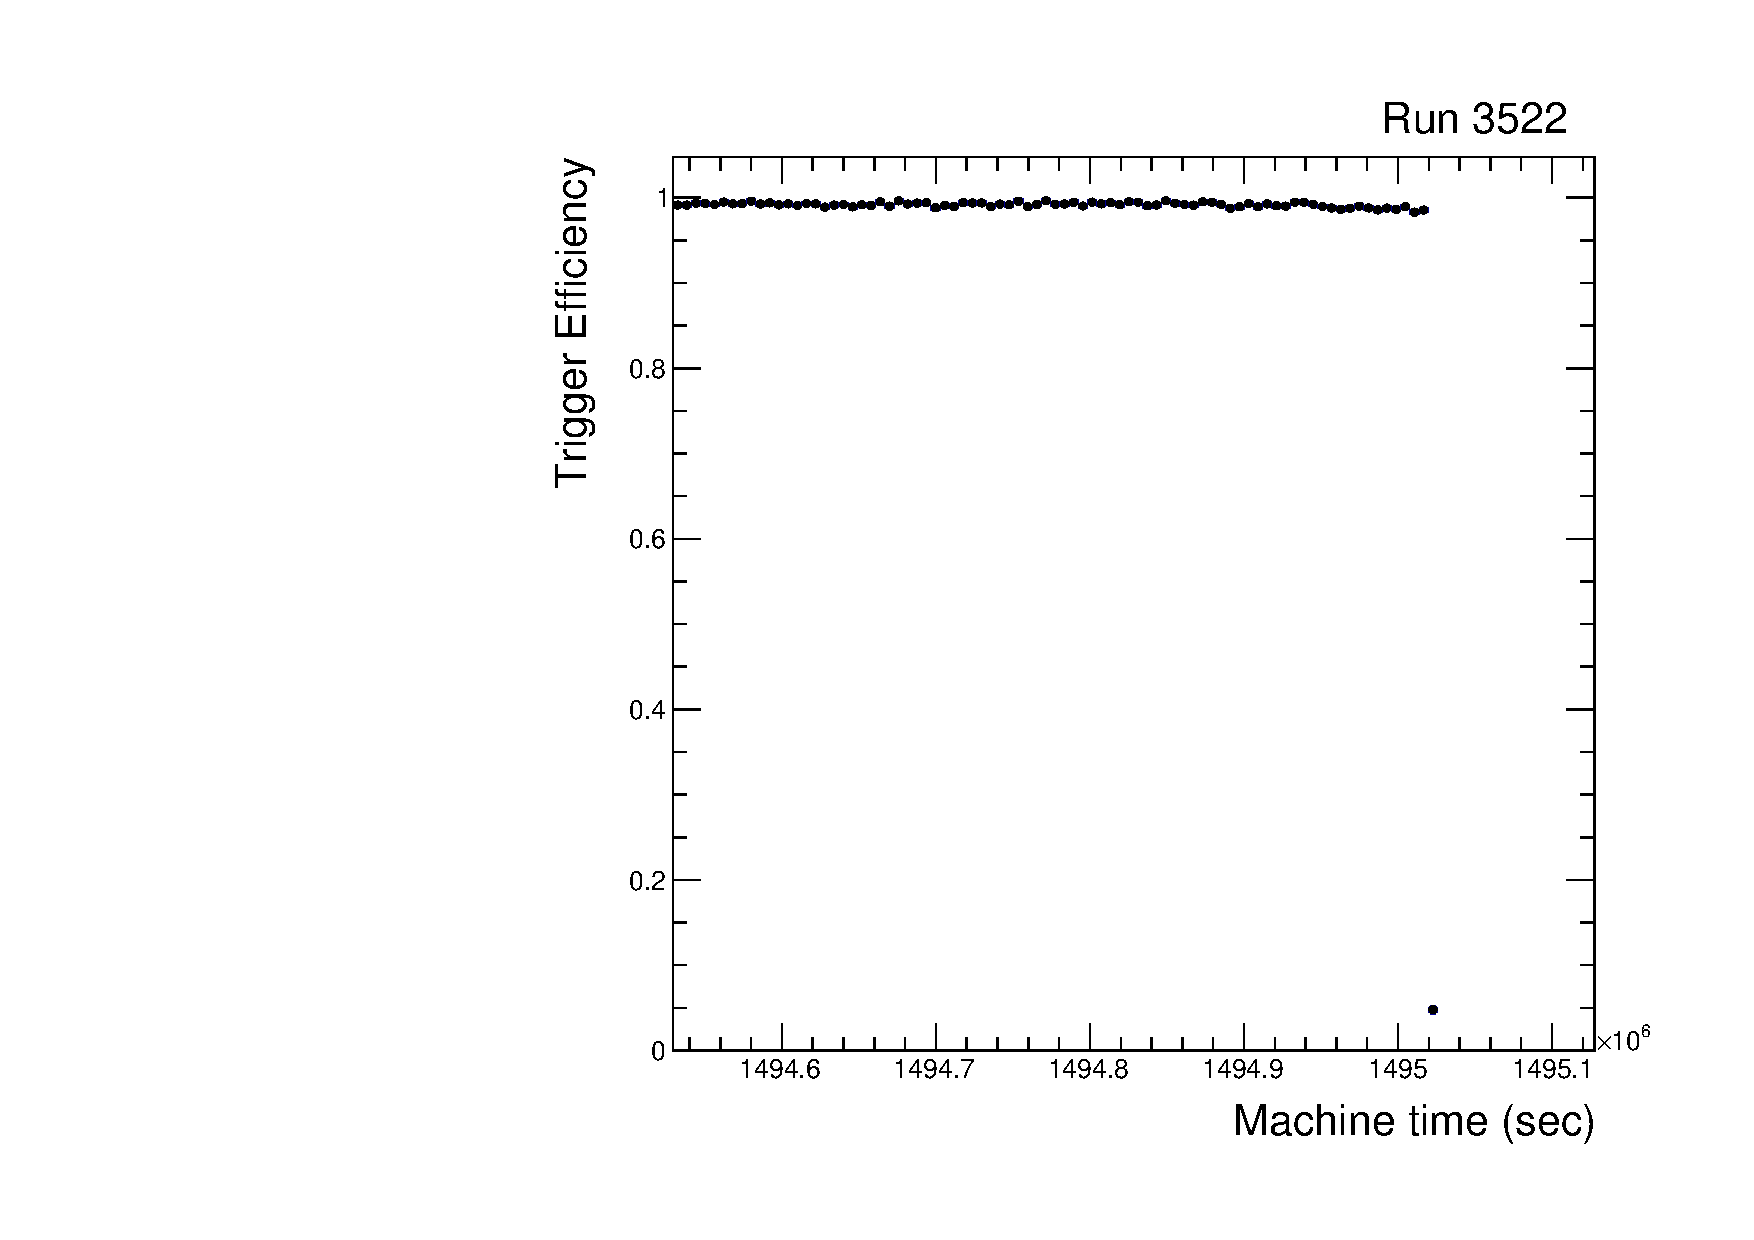
\includegraphics[width=0.48\textwidth]{figures/gbtanalysis3522/tpeff.pdf}
    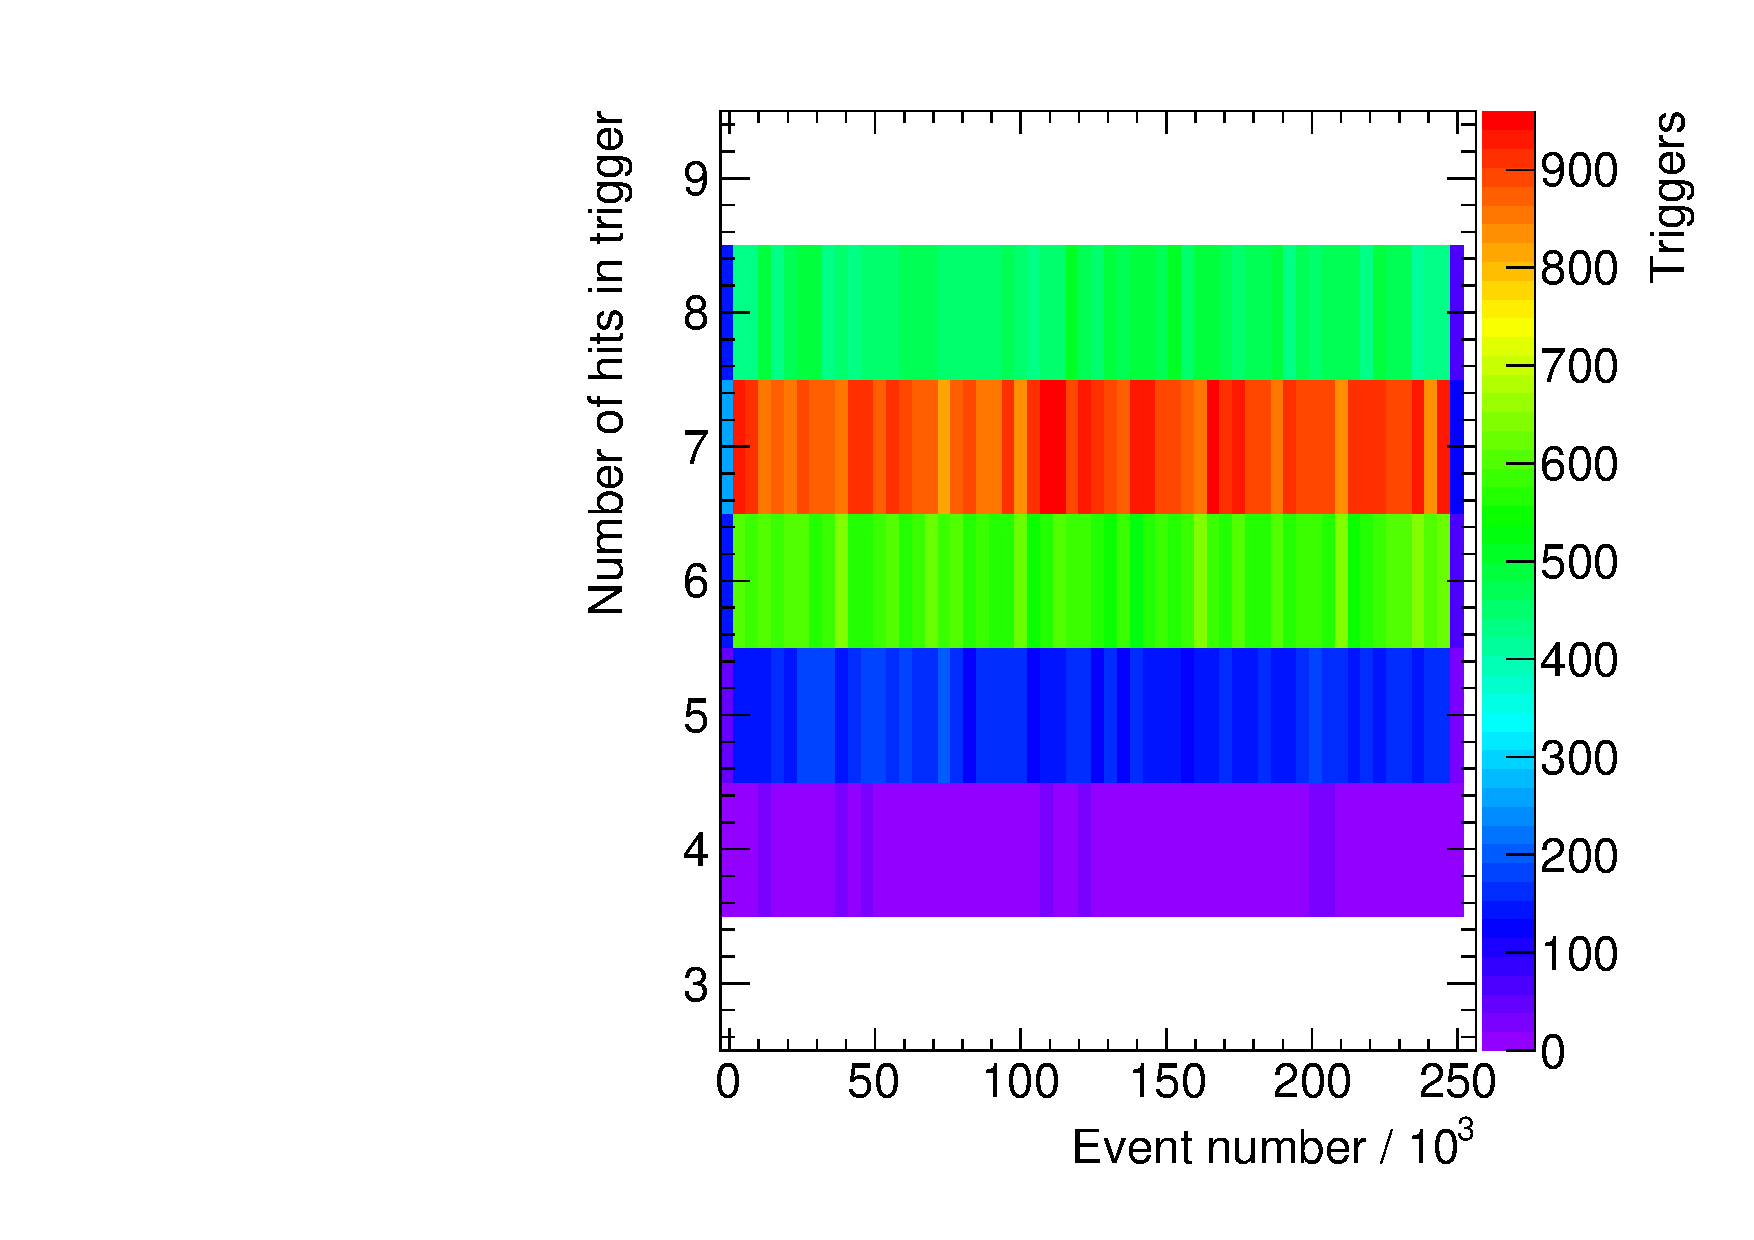
\includegraphics[width=0.48\textwidth]{figures/tuna_analysis/trigger_hits_vs_event.pdf}
  \end{center}
  \vspace{-10pt}
  \caption{The efficiency of a trigger to be matched to a full readout event versus time (left) and the number of hits in the trigger as a function of time (right). Both figures show stable data-taking.}
  \label{fig:lowlevel}
\end{figure}

\begin{figure}[!htpb]
  \begin{center}
    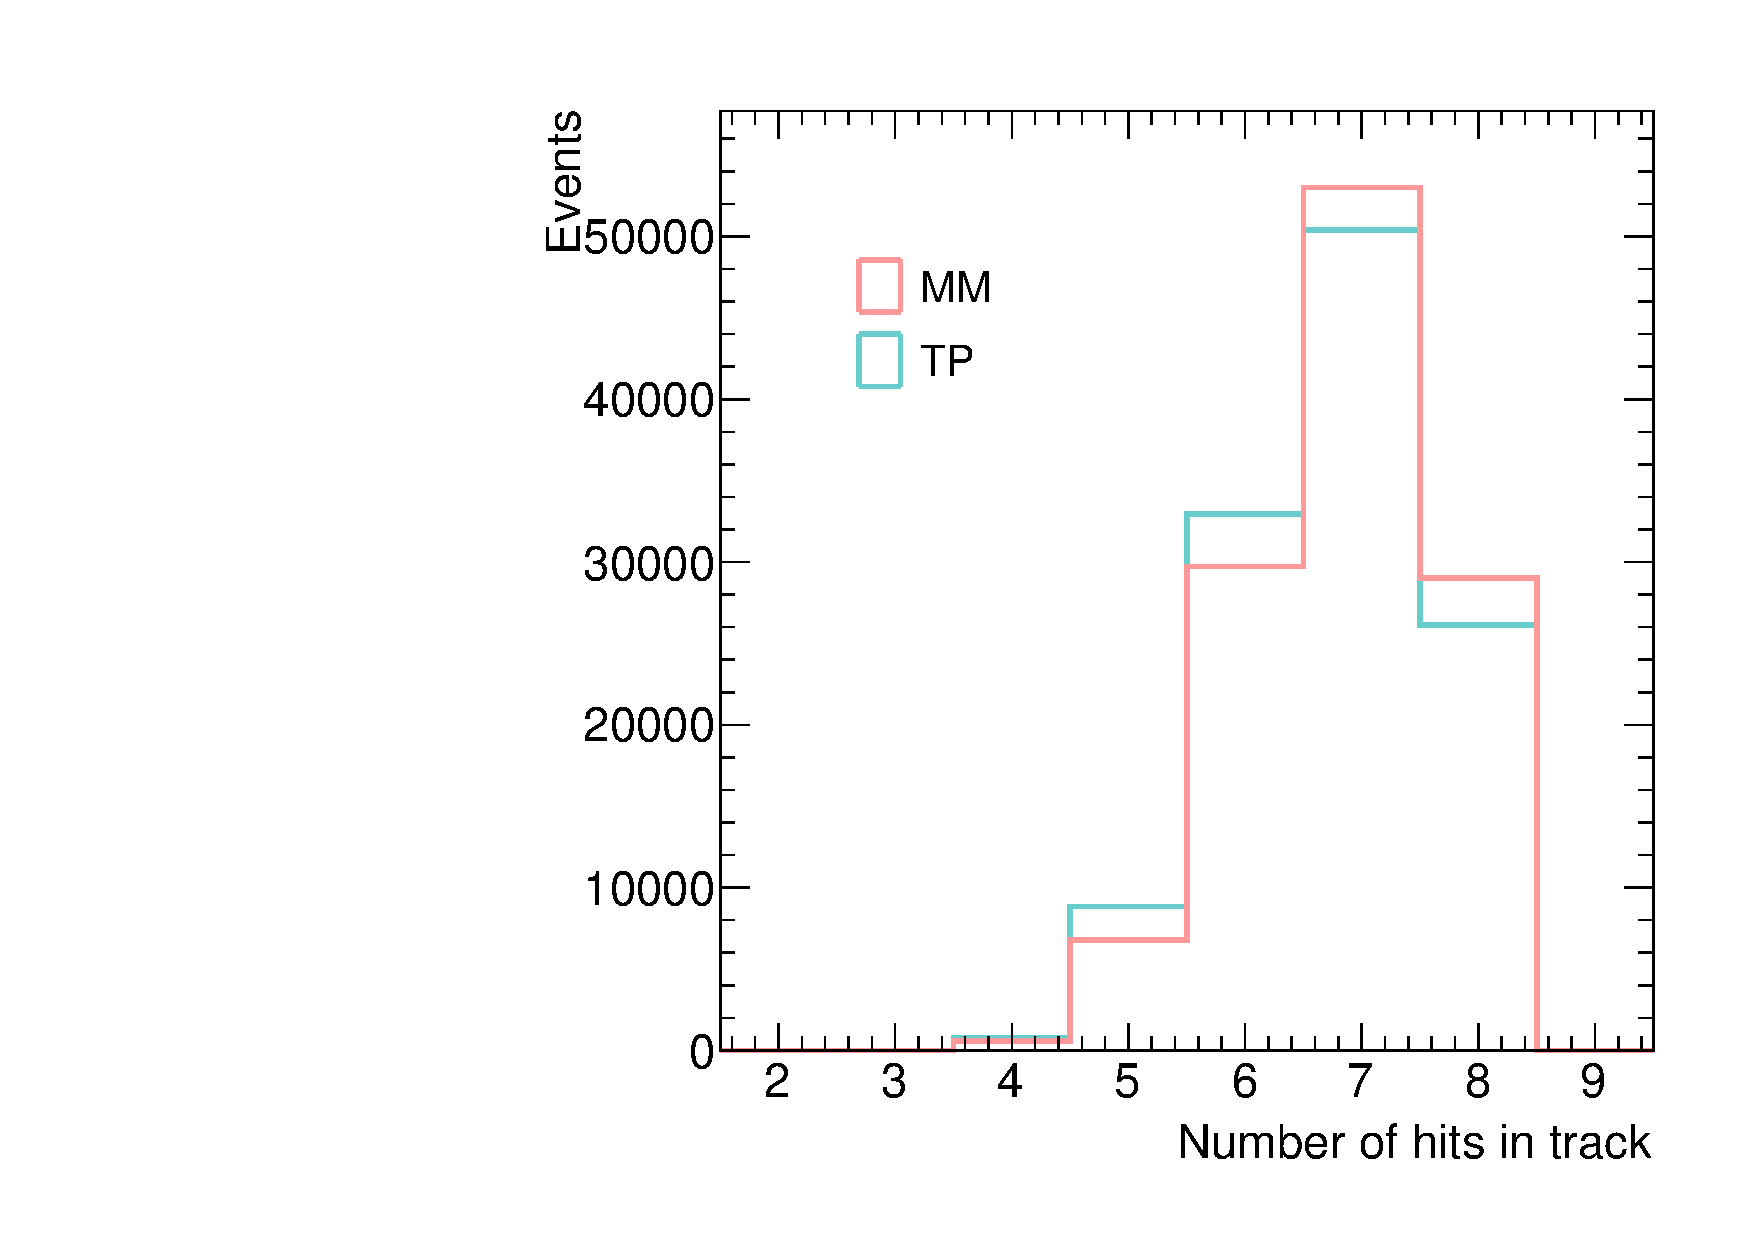
\includegraphics[width=0.48\textwidth]{figures/tuna_analysis/trigger_nart.pdf}
    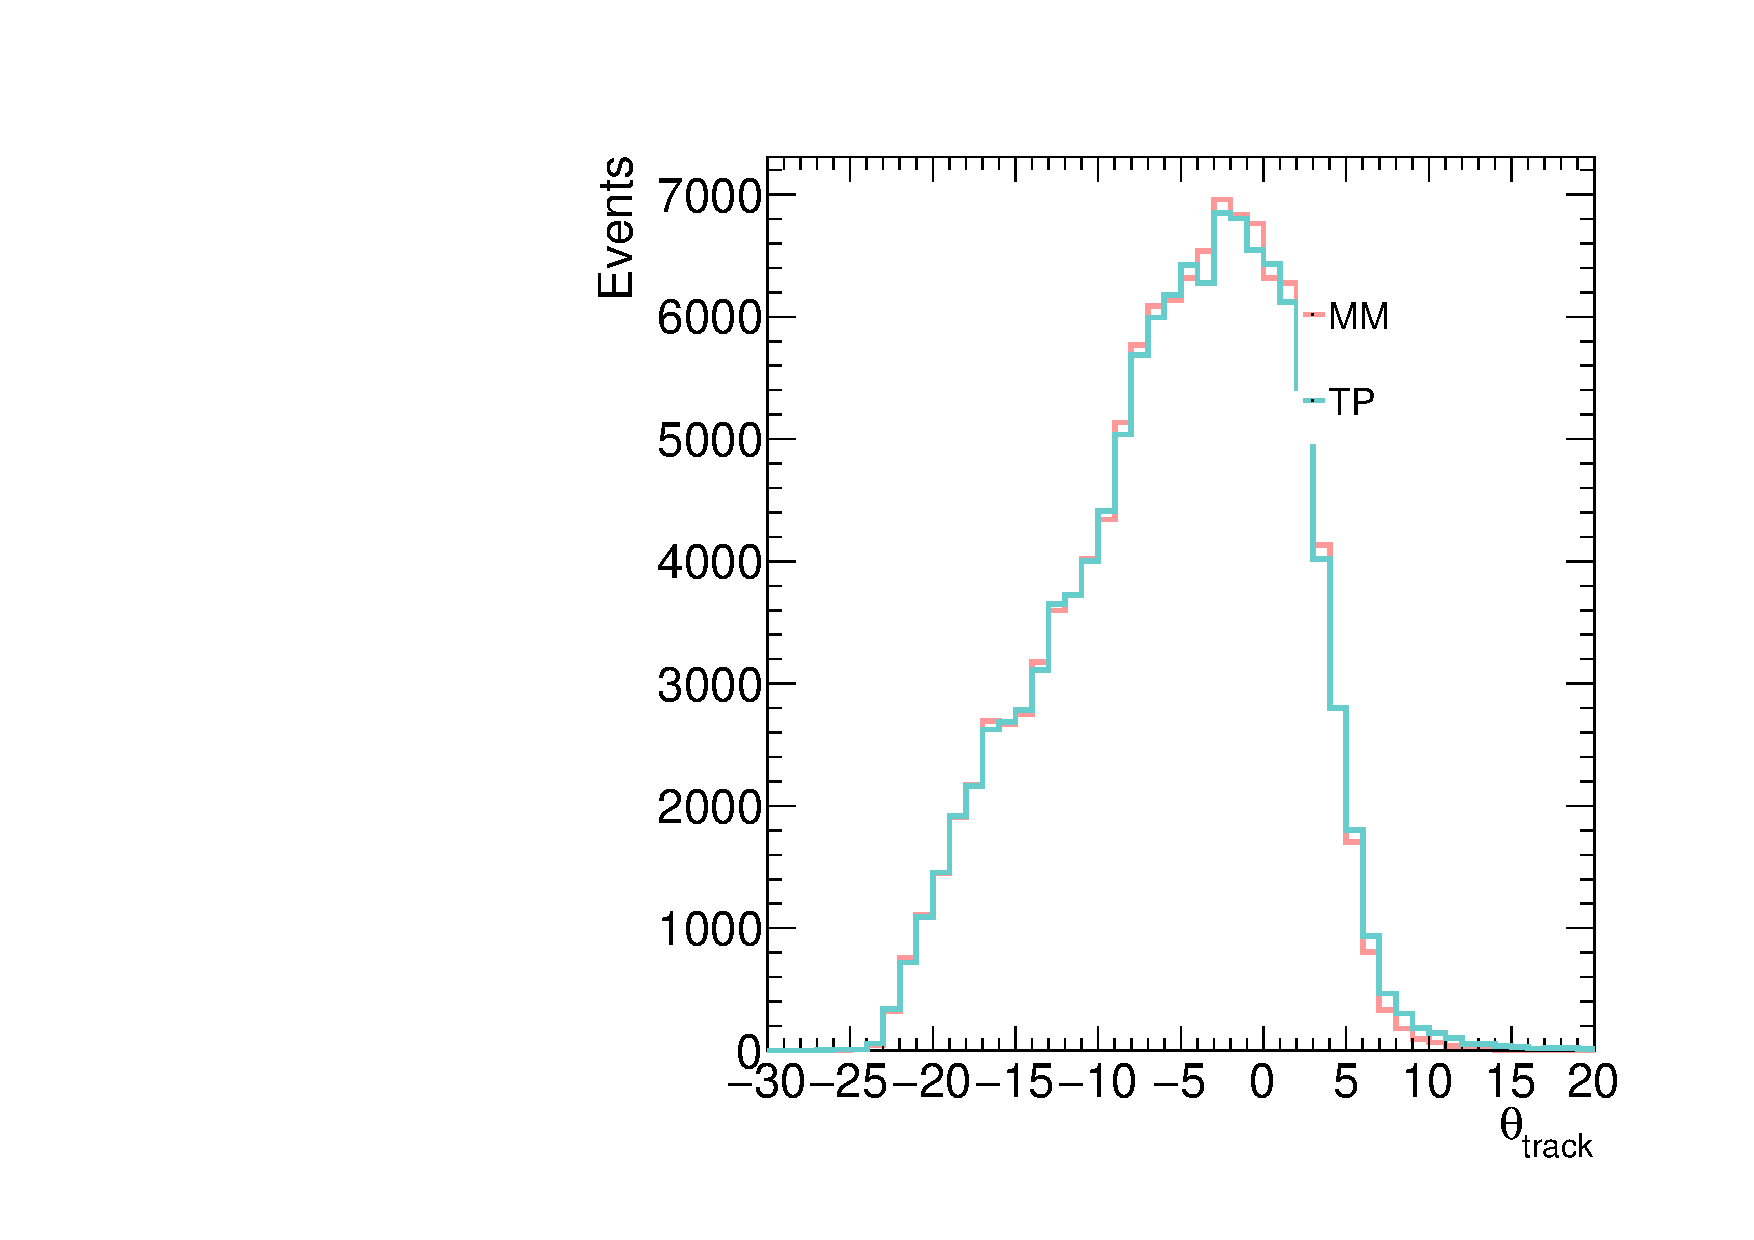
\includegraphics[width=0.48\textwidth]{figures/gbtanalysis3522/ang.pdf}
  \end{center}
  \vspace{-10pt}
  \caption{The number of hits in the MMTP and MM FE tracks (left) and the angle of the tracks (right). The track found by the trigger closely resembles the track found by the full readout, though with slightly fewer hits on average.}
  \label{fig:tp_vs_fe}
\end{figure}

\subsection{Offline roads}
\label{sec:perf-roads}

An additional trigger quality requirement is considered when measuring the resolution of the MMTP. As discussion in Section~\ref{sec:alg-finder}, the road size configured in the FPGA is 1 VMM, or effectively 3 VMMs when including neighboring roads. This allows muons with large incident angle to form triggers in the MMTP, but it is also vulnerable to background hits since the effective road is much larger than needed for a downward-going muon. This vulnerability is less relevant for the NSW implementation of the algorithm because it will use \textit{slope-roads}, which is equivalent to only triggering on downward-going muons when using simple, strip-based roads.

To avoid this vulnerability, the resolution measured is presented in two ways. First, the resolution measured by the MMTP is shown unadulterated. Second, the resolution is shown for triggers which satisfy \textit{offline roads}, to emulate the slope-roads of the NSW implementation. Offline roads are defined relative to the reference track of the full MMFE8 readout. The position of this track is evaluated at each layer, and a road is created around this position. The offline roads in this note are defined as 16 strips (1/4 VMM), with neighbors on either side, which is approximately the size of the slope-roads suggested for the NSW. Therefore an ART hit on a given layer must be within 24 strips of the track to ``satisfy'' the road. A trigger is said to satisfy the offline road if all the hits of the trigger satisfy the road individually.

An important caveat is that even slope-roads cannot be simply defined for stereo planes. Unlike horizontal strips, the slope of a stereo strip measured at one edge of the wedge is different than the slope measured at the other edge. The MMTP defines the slope of a stereo strip as the slope evaluated in the center of the wedge, and as the road size is made smaller, it can become inefficient for tracks traversing the wedge near the edges. Therefore the road size for stereo planes must be larger than for horizontal planes.

In this note, the offline stereo road is made larger by approximately the amount which will be needed at the NSW. This amount is smallest in the region closest to the beamline of the SM1 chamber, and largest in the region farthest from the beamline of the LM2 chamber, as shown in Figure~\ref{fig:stereo_roads}. This corresponds to 13 mm (or 33 strips) and 58 mm (or 144 strips), respectively. The two offline stereo roads in this note are then 1/4 VMM, with neighboring roads, plus either of these tolerances. Coincidentally, an offline road of 1/4 VMM with an extra 144 strips is 192 strips, or 3 VMMs, so no offline requirement is needed on top of the 1 VMM road required online by the FPGA.

\begin{figure}[!htpb]
  \begin{center}
    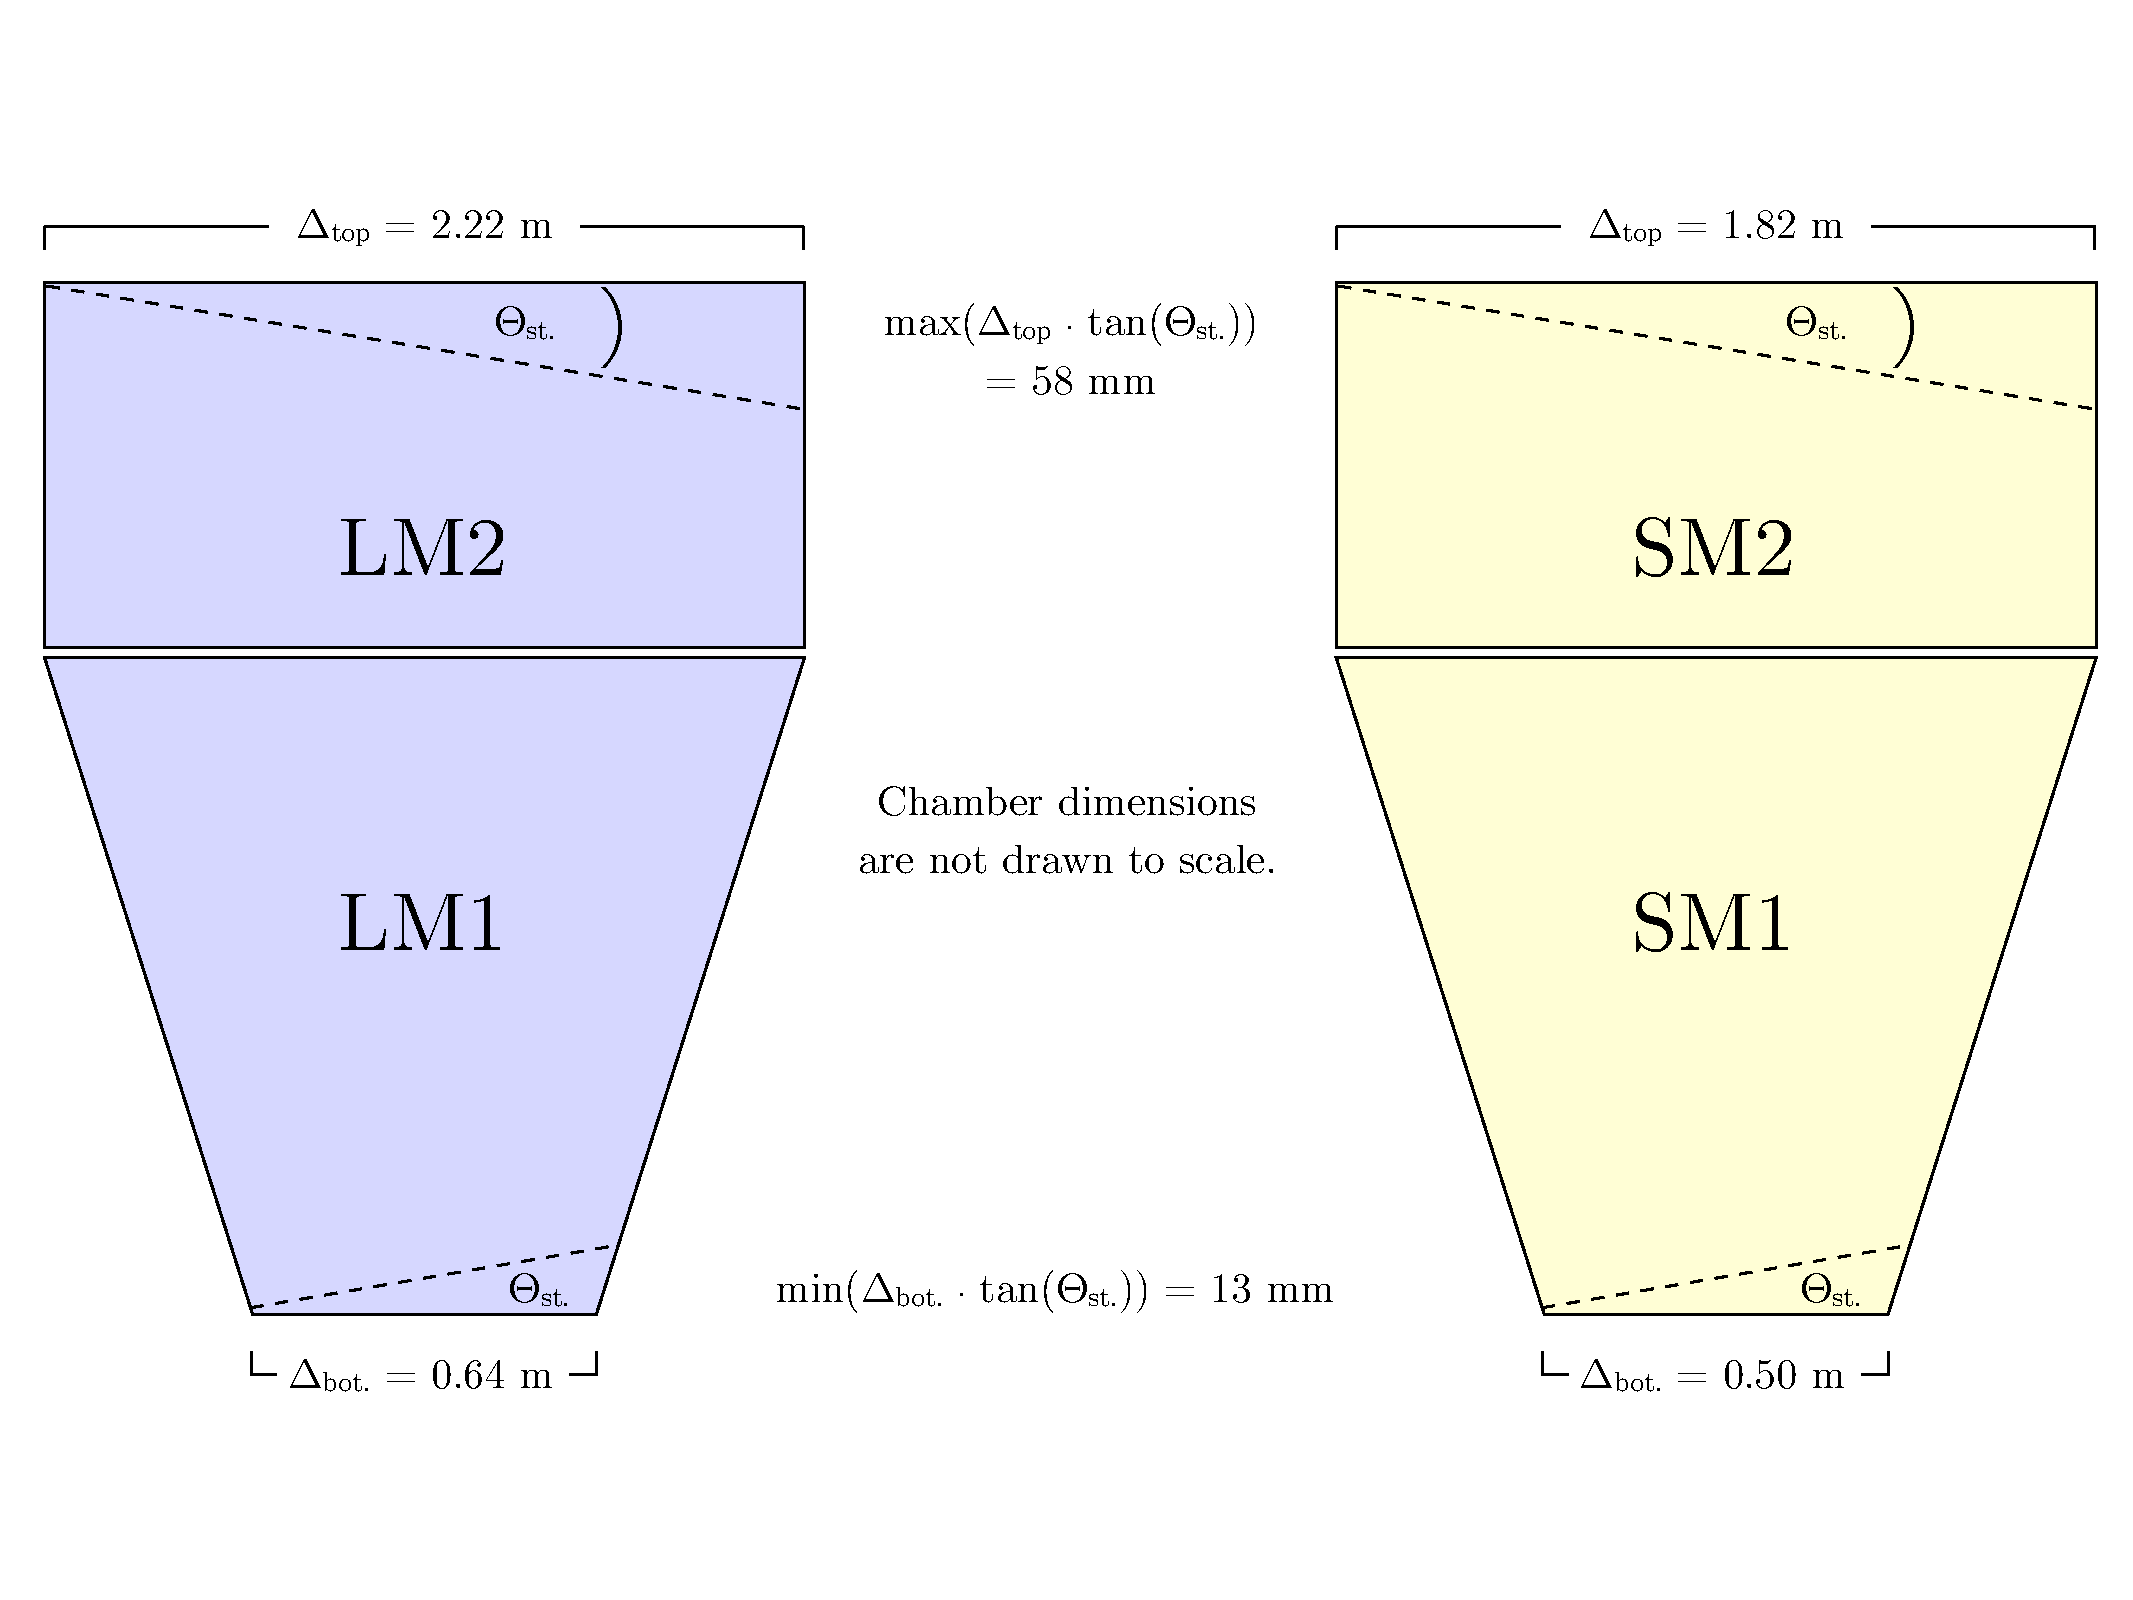
\includegraphics[width=1.0\textwidth]{figures/cartoons/stereo_roads.pdf}
  \end{center}
  \vspace{-10pt}
  \caption{A drawing of the Micromegas wedges with the dimensions specified by the NSW. The stereo strips require larger roads than the horizontal strips because they cover between 13 and 58 mm of the detector in the direction of the precision coordinate.}
  \label{fig:stereo_roads}
\end{figure}

\subsection{Spatial and angular resolution}
\label{sec:perf-res}

The spatial resolutions measured with cosmic data are shown in Figures~\ref{fig:xres} and~\ref{fig:yres}. The $x$ resolution is measured as the difference between the average $x$ position of the trigger hits on the $X$ planes and the $x$ position of the fitted MMFE8 track evaluated at the average $z$ position of the trigger hits. Calculating the average of trigger $X$ hits corresponds directly to calculating the average of $X$ slopes at the NSW, also known as $m_X^\text{global}$, which dominates the $\eta$ measurement. The $y$ resolution is measured as the difference between the difference of average $x$ position of $U$ and $V$ planes, with the geometric factor $\frac{1}{2\ \text{tan}\theta_\text{st.}}$, and the $y$ position of the fitted MMFE8 track evalutated at the average $z$ position of the trigger stereo hits. The trigger $y$ measurement is adjusted to account for the slope of the track in the $x-z$ plane. Calculating the difference of the average trigger $U$ and $V$ hits corresponds directly to calculating the difference of the average $U$ and $V$ slopes at the NSW, also known as the non-precision slope, which dominates the $\phi$ measurement.

The $x$ and $y$ resolution improves significantly when requiring tighter offline roads, as expected. The RMS of 0.4 mm (29.3 mm) for the $x$ ($y$) resolution is comparable to what is reported in the TDR. Even with offline roads, however, the distribution seems to reflect two populations of tracks, one sharply peaked at zero and one broadly peaked at zero. The broader distribution is likely caused by $\delta$-rays as the muon passes through the chamber. Two event displays of this feature are shown in Figure~\ref{fig:deltarays}. This motivates using the smallest possible road size at the NSW, for horizontal and stereo planes, to suppress both uncorrelated background hits (e.g. noise) and correlated background hits (e.g. $\delta$-rays).

\begin{figure}[!htpb]
  \begin{center}
    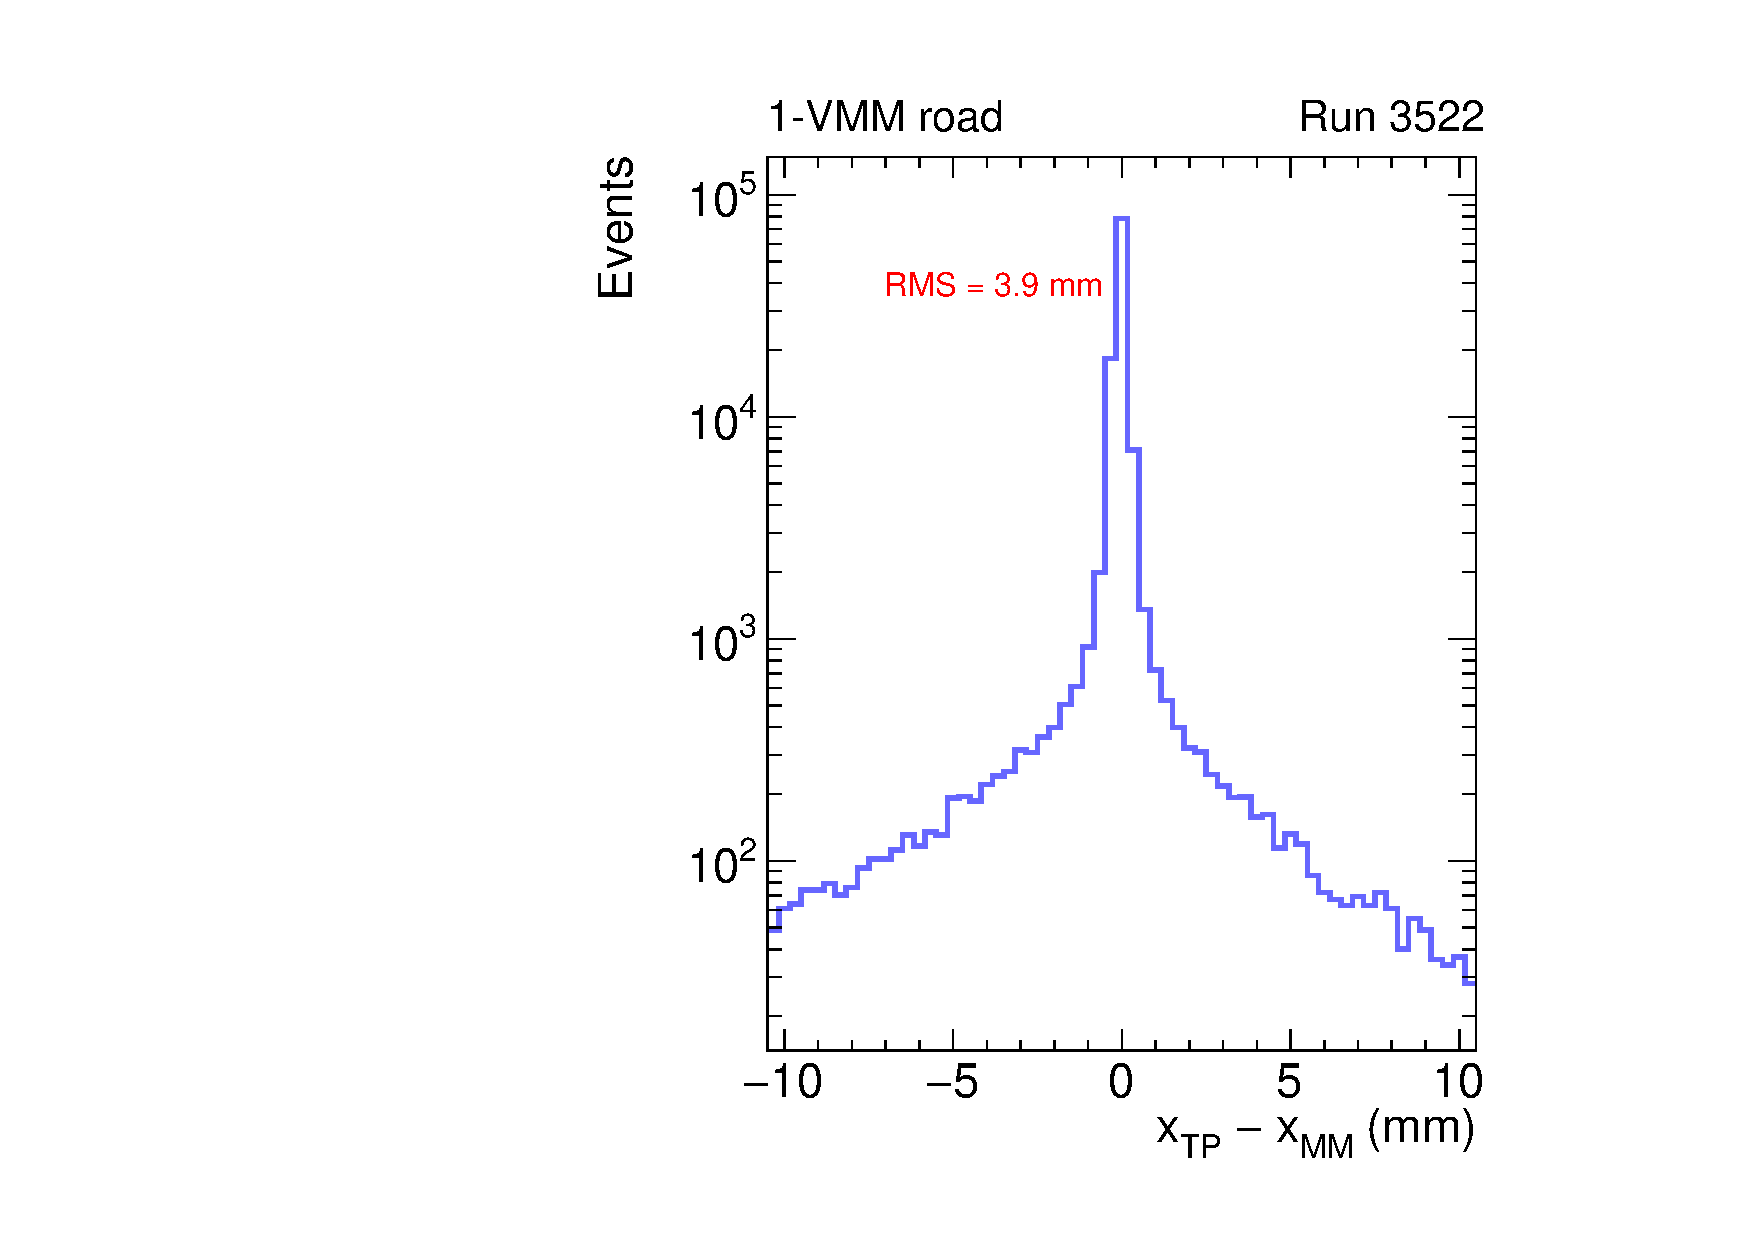
\includegraphics[width=0.48\textwidth]{figures/gbtanalysis3522/TP_xres_full.pdf}
    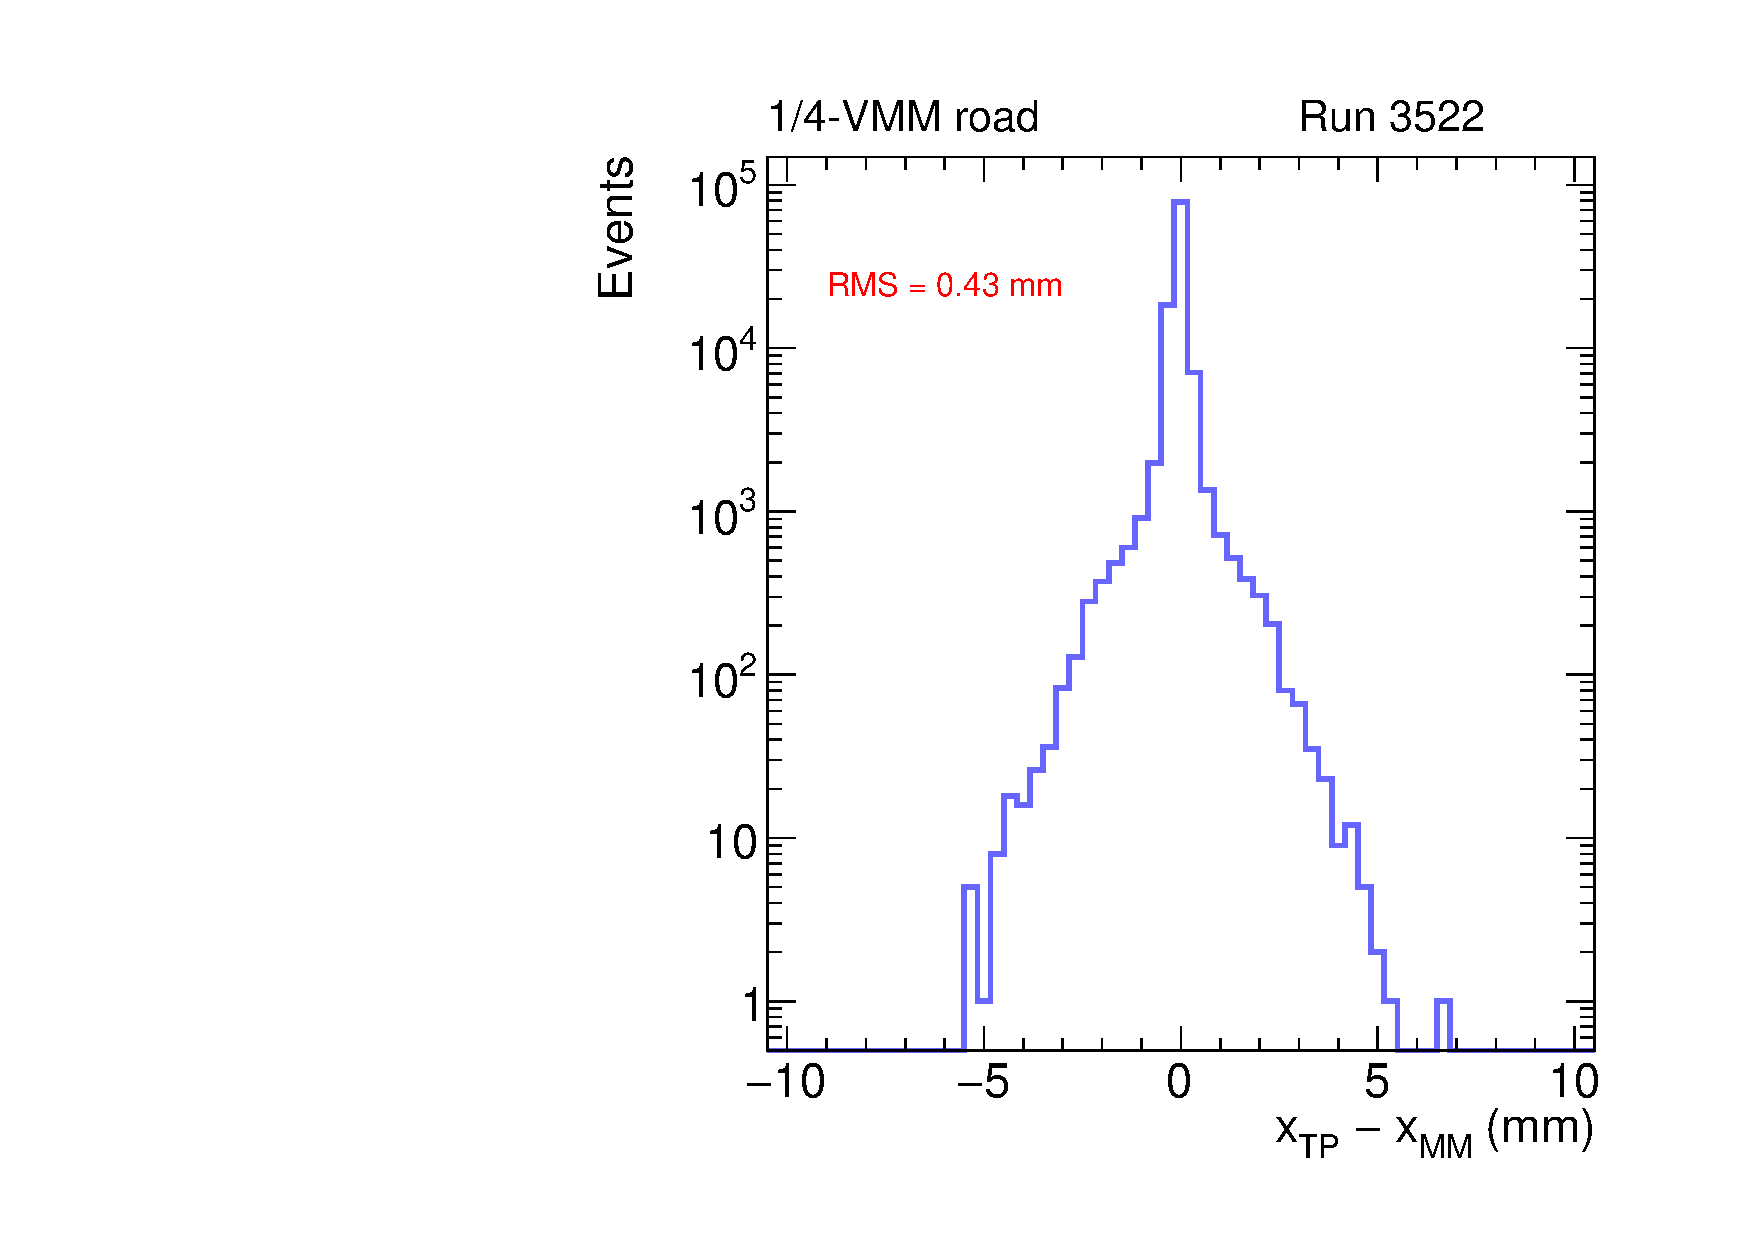
\includegraphics[width=0.48\textwidth]{figures/gbtanalysis3522/TP_xres.pdf}
  \end{center}
  \vspace{-10pt}
  \caption{The $x$ resolution of the MMTP relative to the full readout, using 1-VMM online roads (left) and 1/4-VMM offline roads (right), as discussed in Section~\ref{sec:perf-roads}. The tails of the resolution are greatly suppressed with smaller roads.}
  \label{fig:xres}
\end{figure}

\begin{figure}[!htpb]
  \begin{center}
    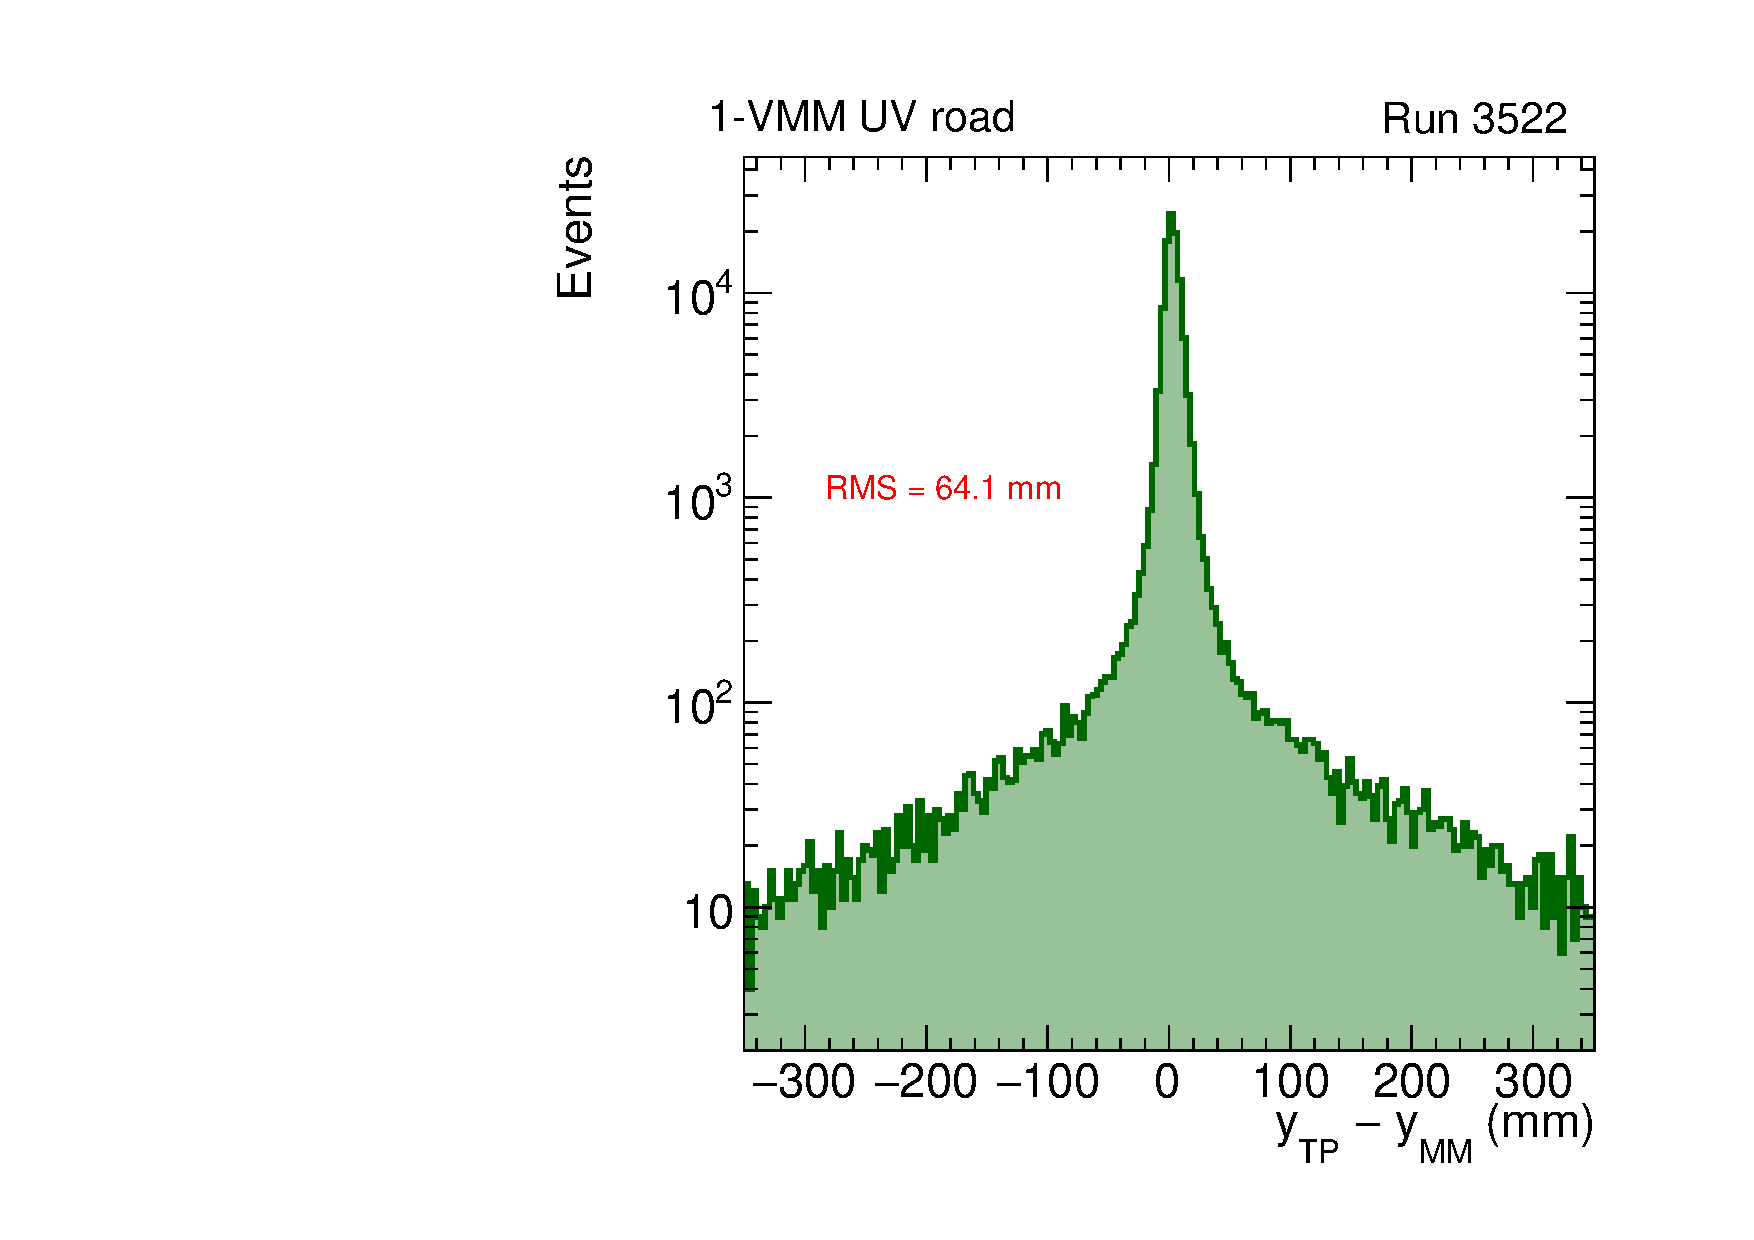
\includegraphics[width=0.48\textwidth]{figures/gbtanalysis3522/TP_yres_1road.pdf}
    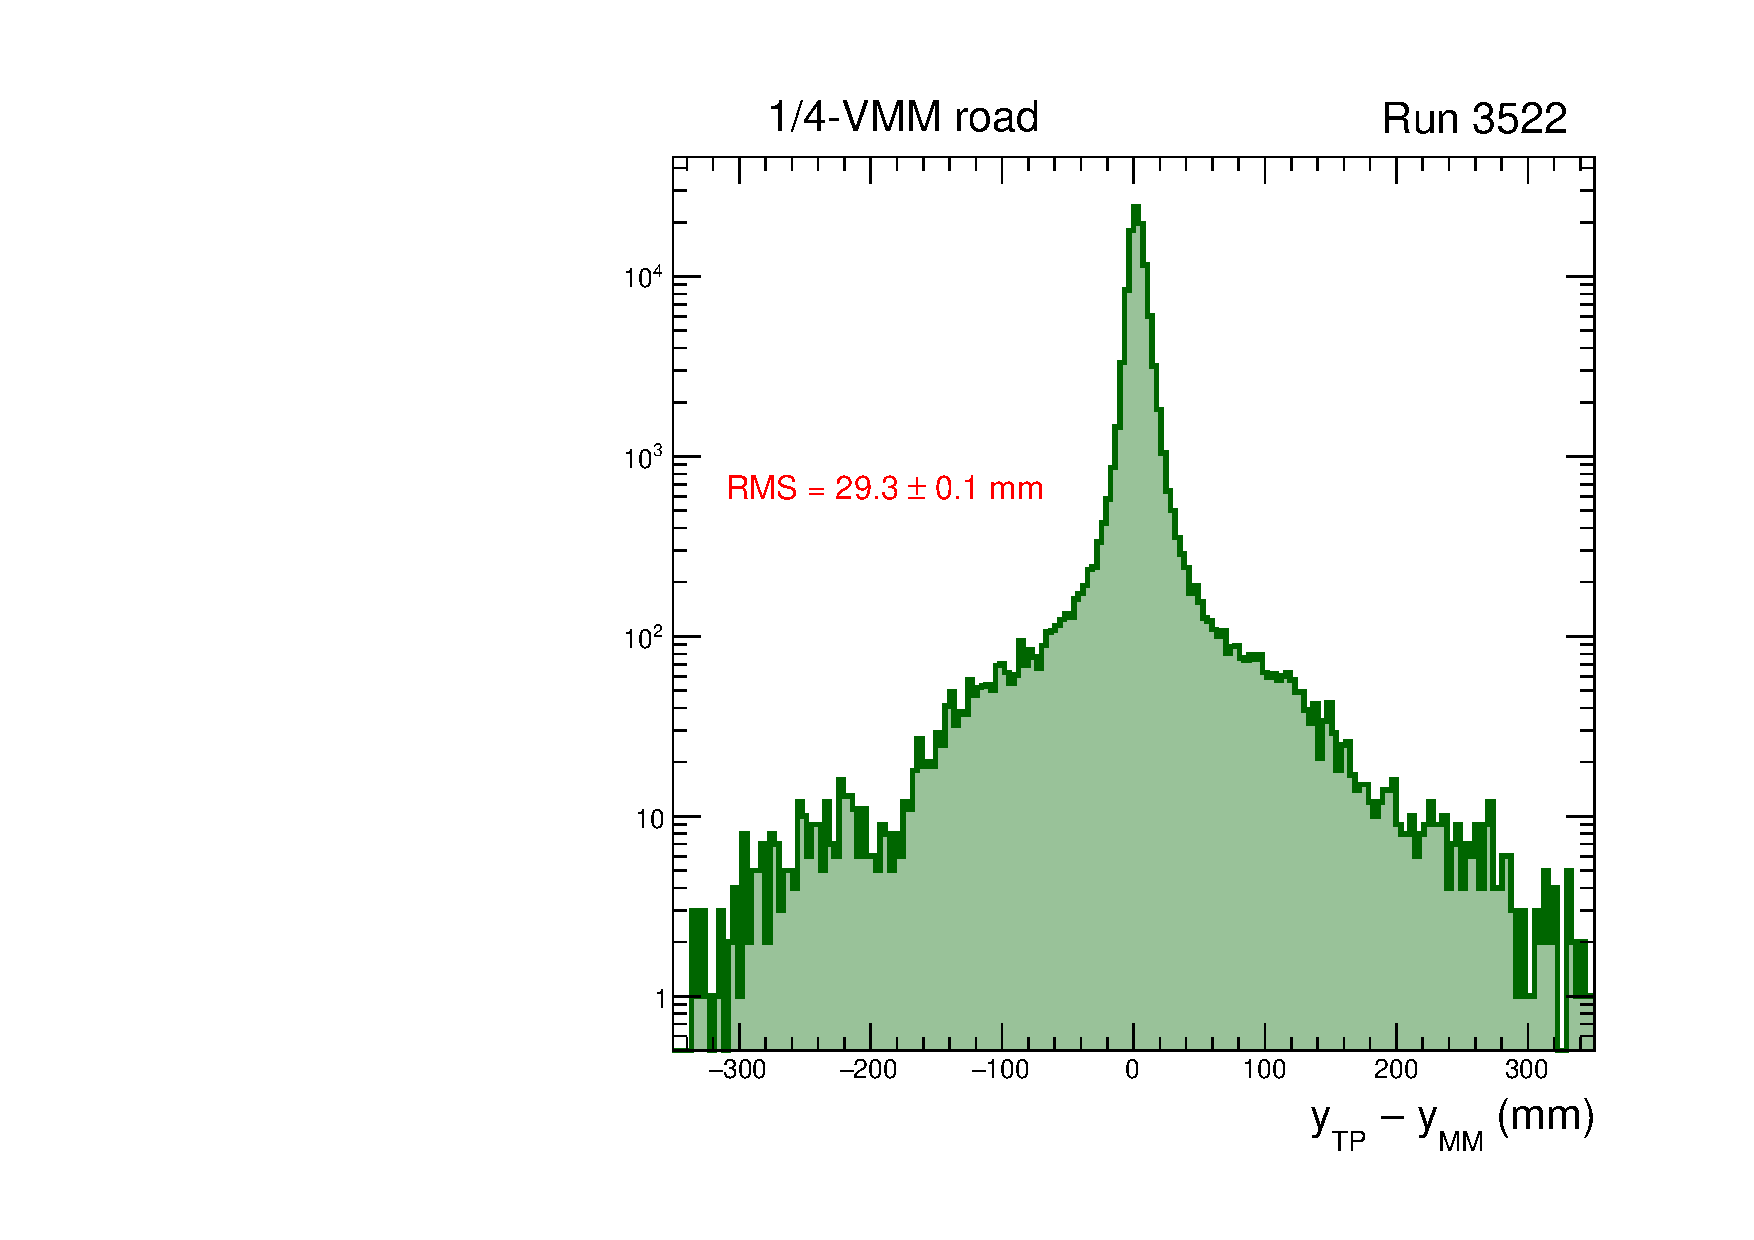
\includegraphics[width=0.48\textwidth]{figures/gbtanalysis3522/TP_yres_smallroad.pdf}
  \end{center}
  \vspace{-10pt}
  \caption{The $y$ resolution of the MMTP relative to the full readout, using 1-VMM online roads (left) and 1/4-VMM offline roads (right), as discussed in Section~\ref{sec:perf-roads}. The tails of the resolution are greatly suppressed with smaller roads.}
  \label{fig:yres}
\end{figure}

\begin{figure}[!htpb]
  \begin{center}
    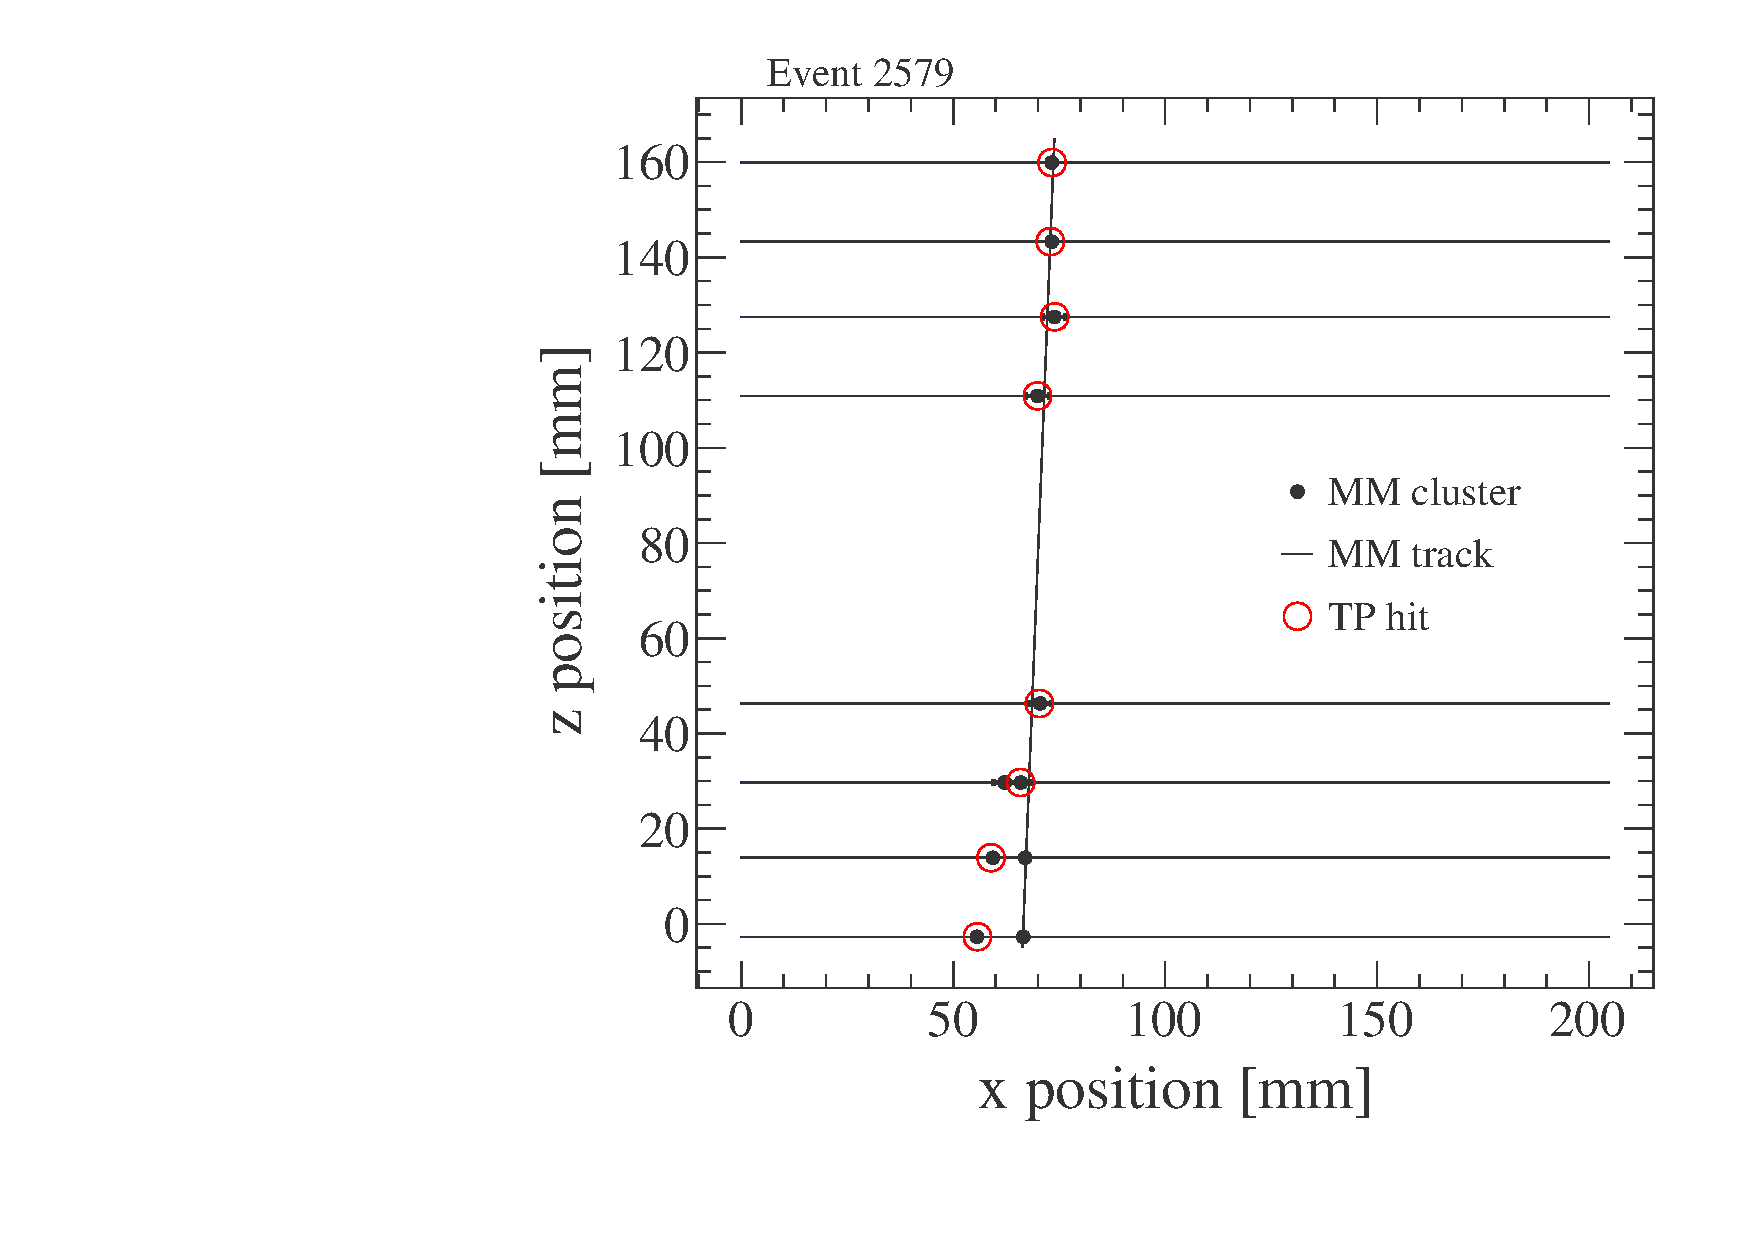
\includegraphics[width=0.48\textwidth]{figures/event_displays/display_02579.pdf}
    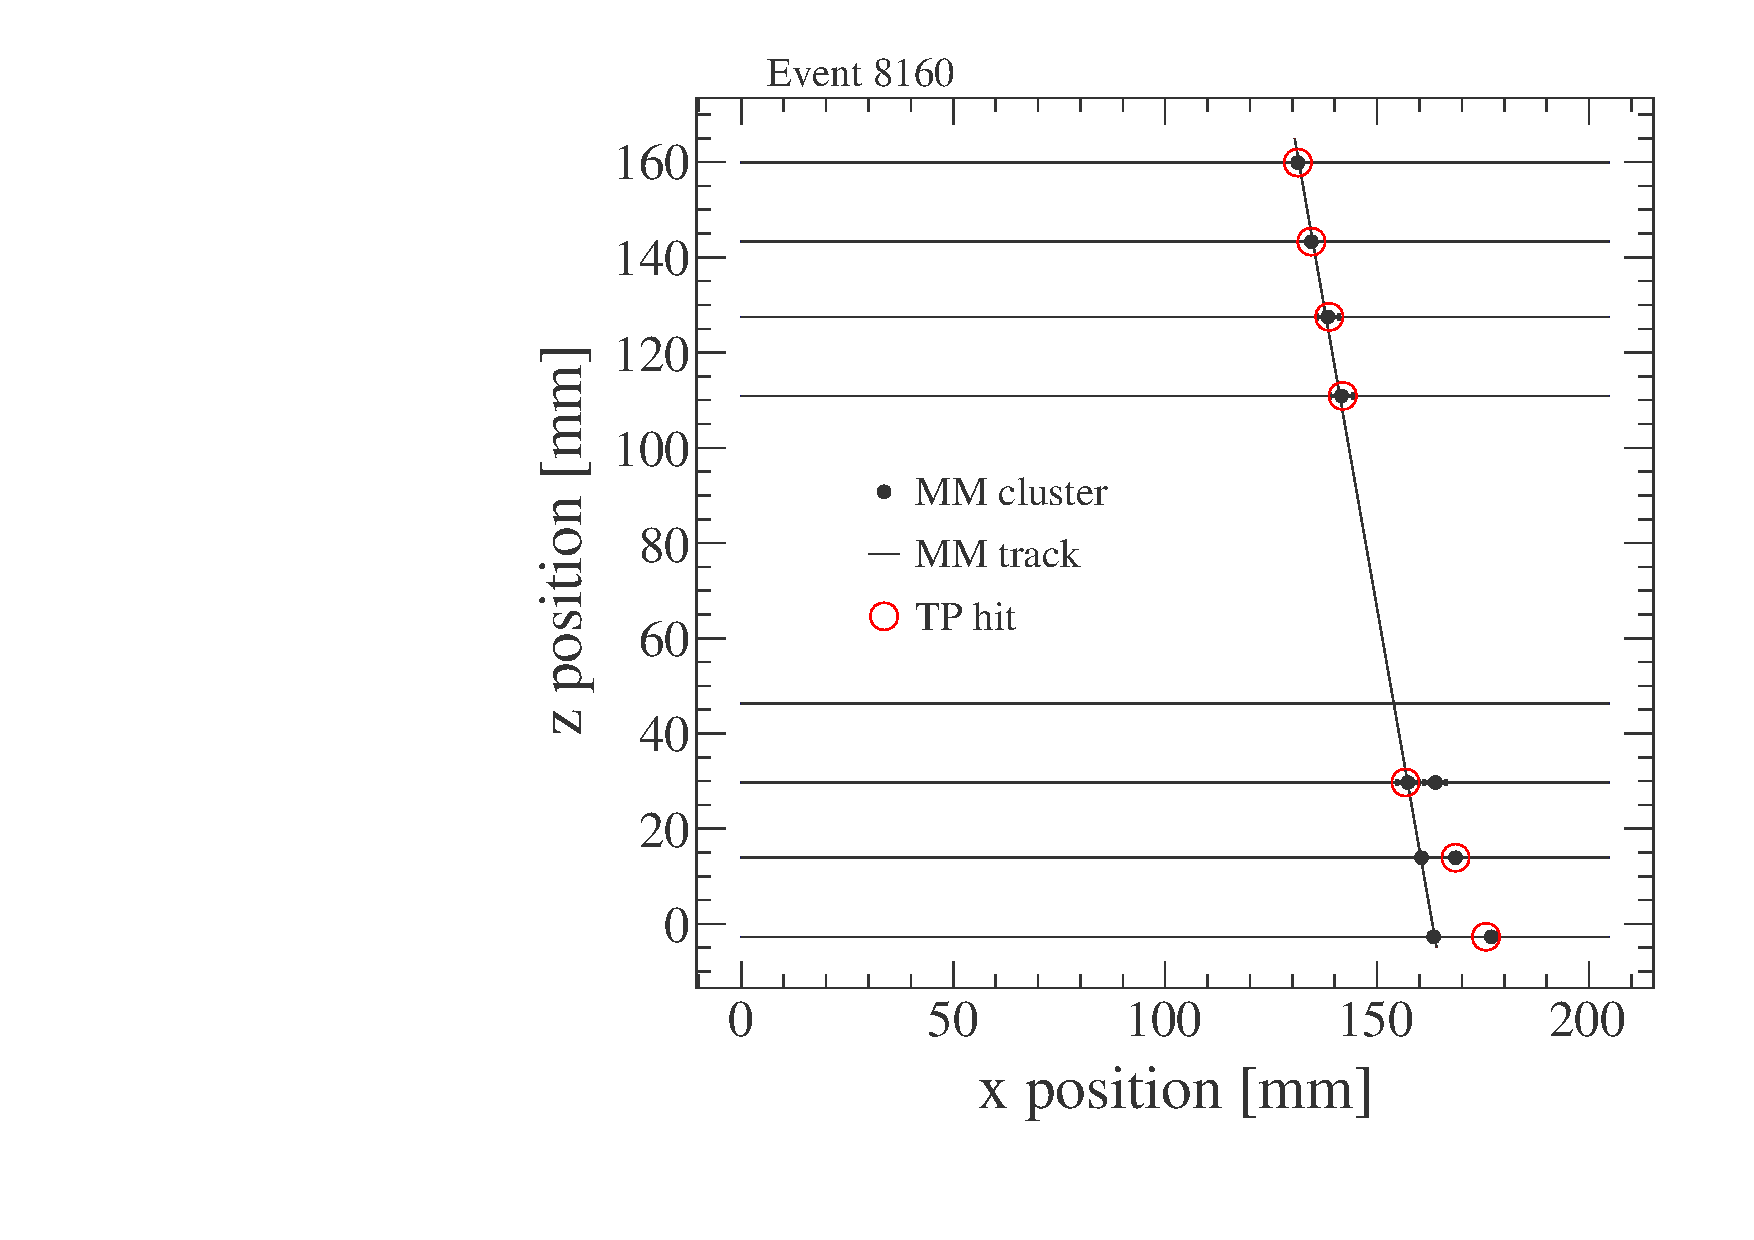
\includegraphics[width=0.48\textwidth]{figures/event_displays/display_08160.pdf}
  \end{center}
  \vspace{-10pt}
  \caption{Two event displays likely to include delta rays. The black circles are clusters from the full MMFE8 readout, the black line is the fit to the clusters, and the red circles are the hits chosen by the MMTP. In both cases, the MMTP chooses hits from the delta ray.}
  \label{fig:deltarays}
\end{figure}

The angular resolution measured with cosmic data is shown in Figure~\ref{fig:thetares}. The $\theta$ resolution is measured as the difference between the slope calculated online by the MMTP FPGA and the slope of the fitted MMFE8 track, after converting each slope to an angle. The online slope is exactly the slope which will be calculated online at the NSW, also known as $m_X^\text{local}$. The resolution of $m_X^\text{local}$ dominates the resolution of $\Delta\theta$, which measures the consistency of the trigger with the interaction point. The measured $\theta$ resolution is comparable to what is reported in the TDR, and it improves similarly with smaller road sizes, as expected.

The angular and spatial resolution are shown simultaneously in Figure~\ref{fig:xthetares}. There is a clear correlation between $x$ and $\theta$ in the case of MMTP measurements which disagree significantly with the full MMFE8 readout, since they are equally affected by background hits in the $X$ planes. In Figure~\ref{fig:xthetares} (left), the long tails are dominated by uncorrelated background hits (noise). In Figure~\ref{fig:xthetares} (right), the tails have contributions from uncorrelated (noise) and correlated ($\delta$-rays) background hits.

\begin{figure}[!htpb]
  \begin{center}
    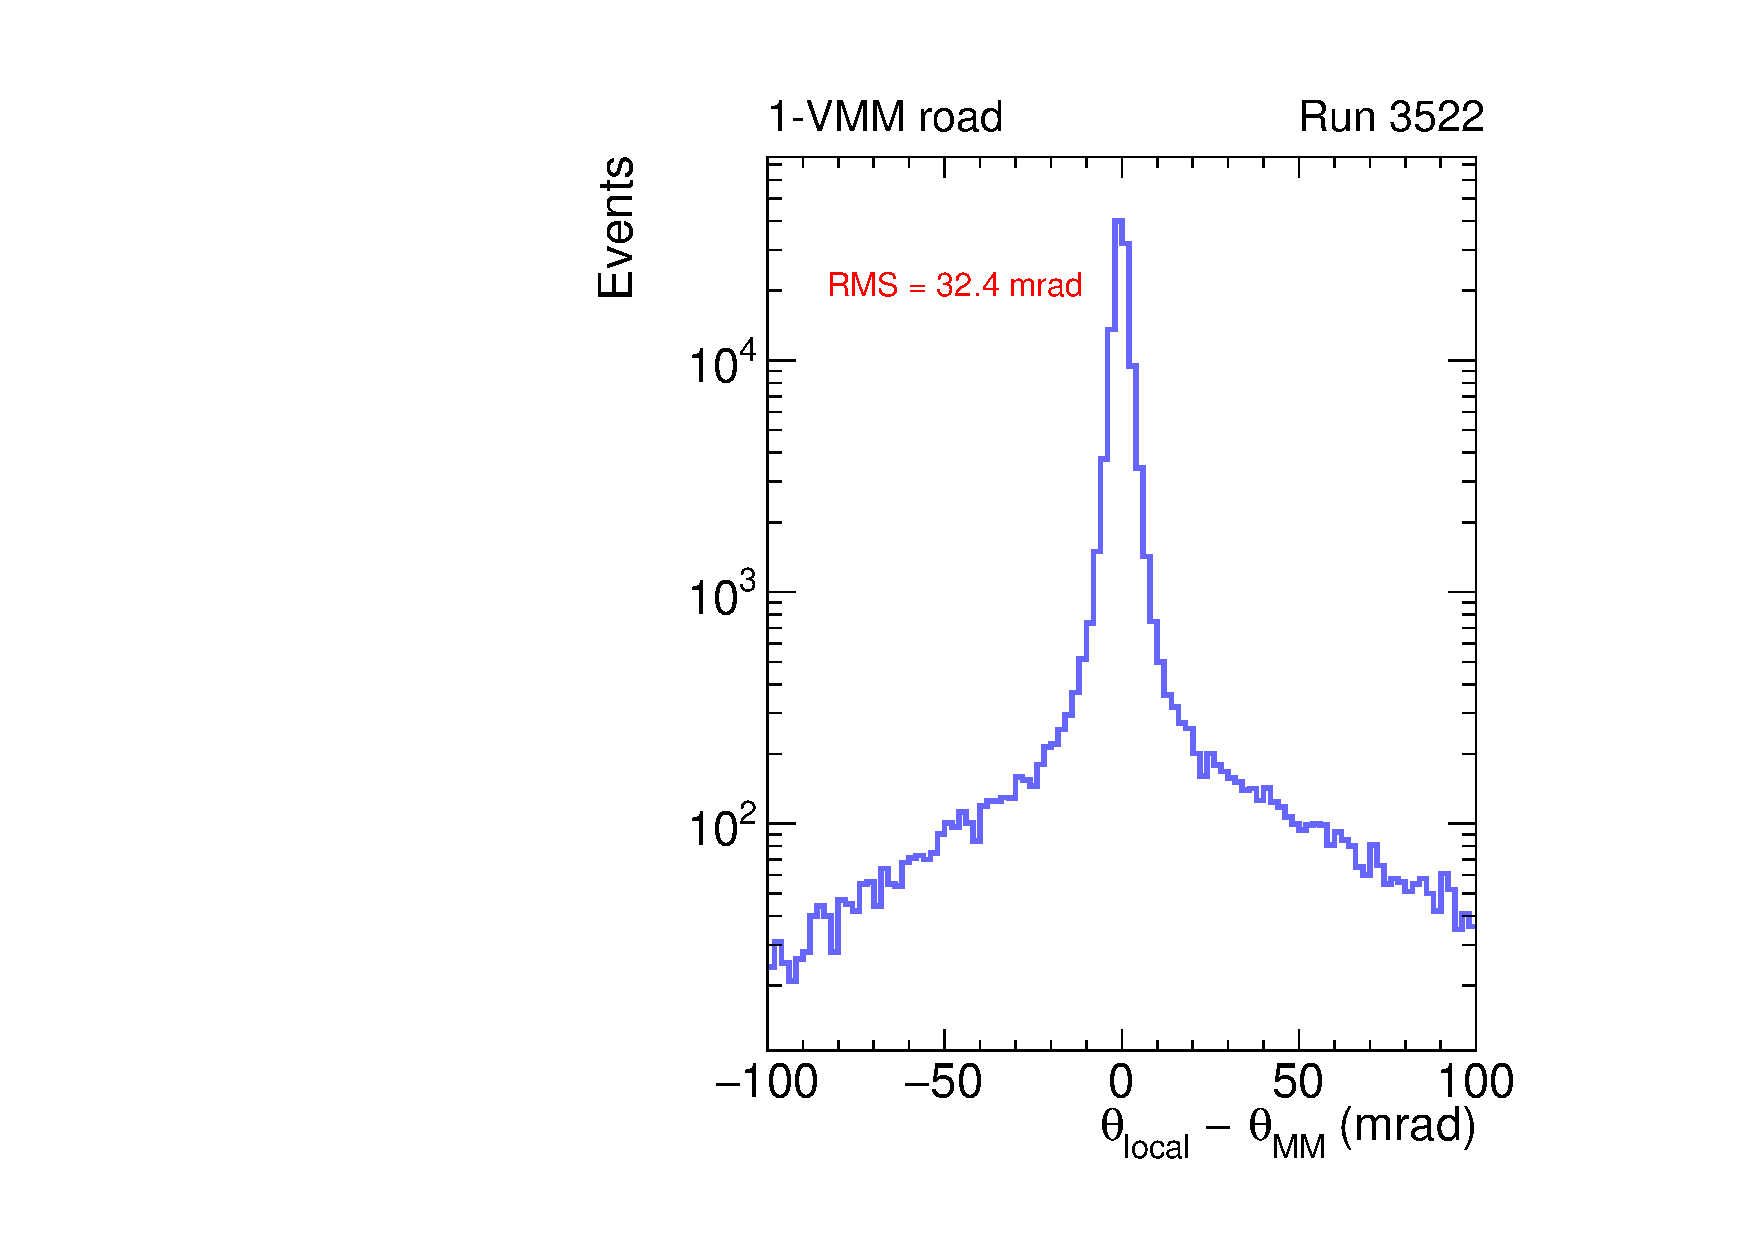
\includegraphics[width=0.48\textwidth]{figures/gbtanalysis3522/TP_angres_full.pdf}
    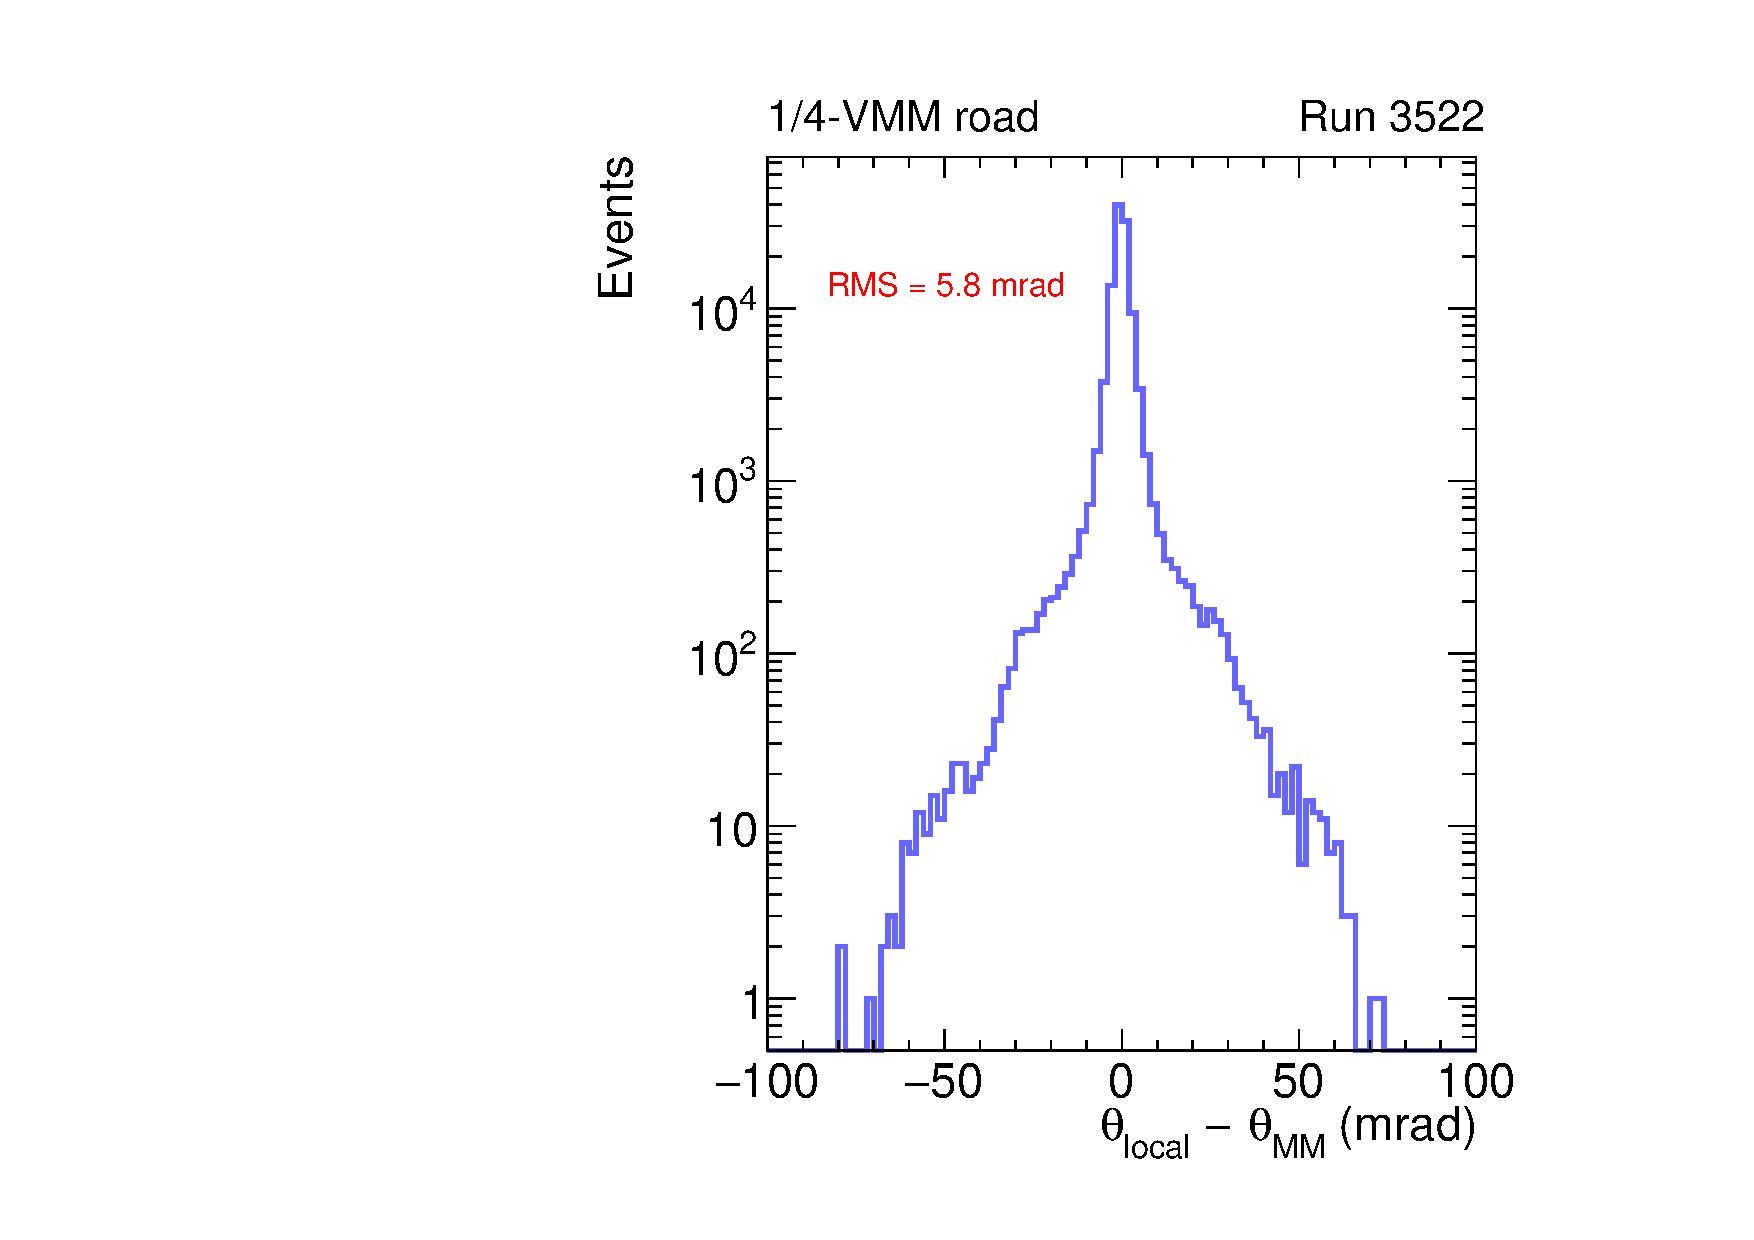
\includegraphics[width=0.48\textwidth]{figures/gbtanalysis3522/TP_angres.pdf}
  \end{center}
  \vspace{-10pt}
  \caption{The $\theta$ resolution of the MMTP relative to the full readout, using 1-VMM online roads (left) and 1/4-VMM offline roads (right), as discussed in Section~\ref{sec:perf-roads}. The tails of the resolution are greatly suppressed with smaller roads.}
  \label{fig:thetares}
\end{figure}

\begin{figure}[!htpb]
  \begin{center}
    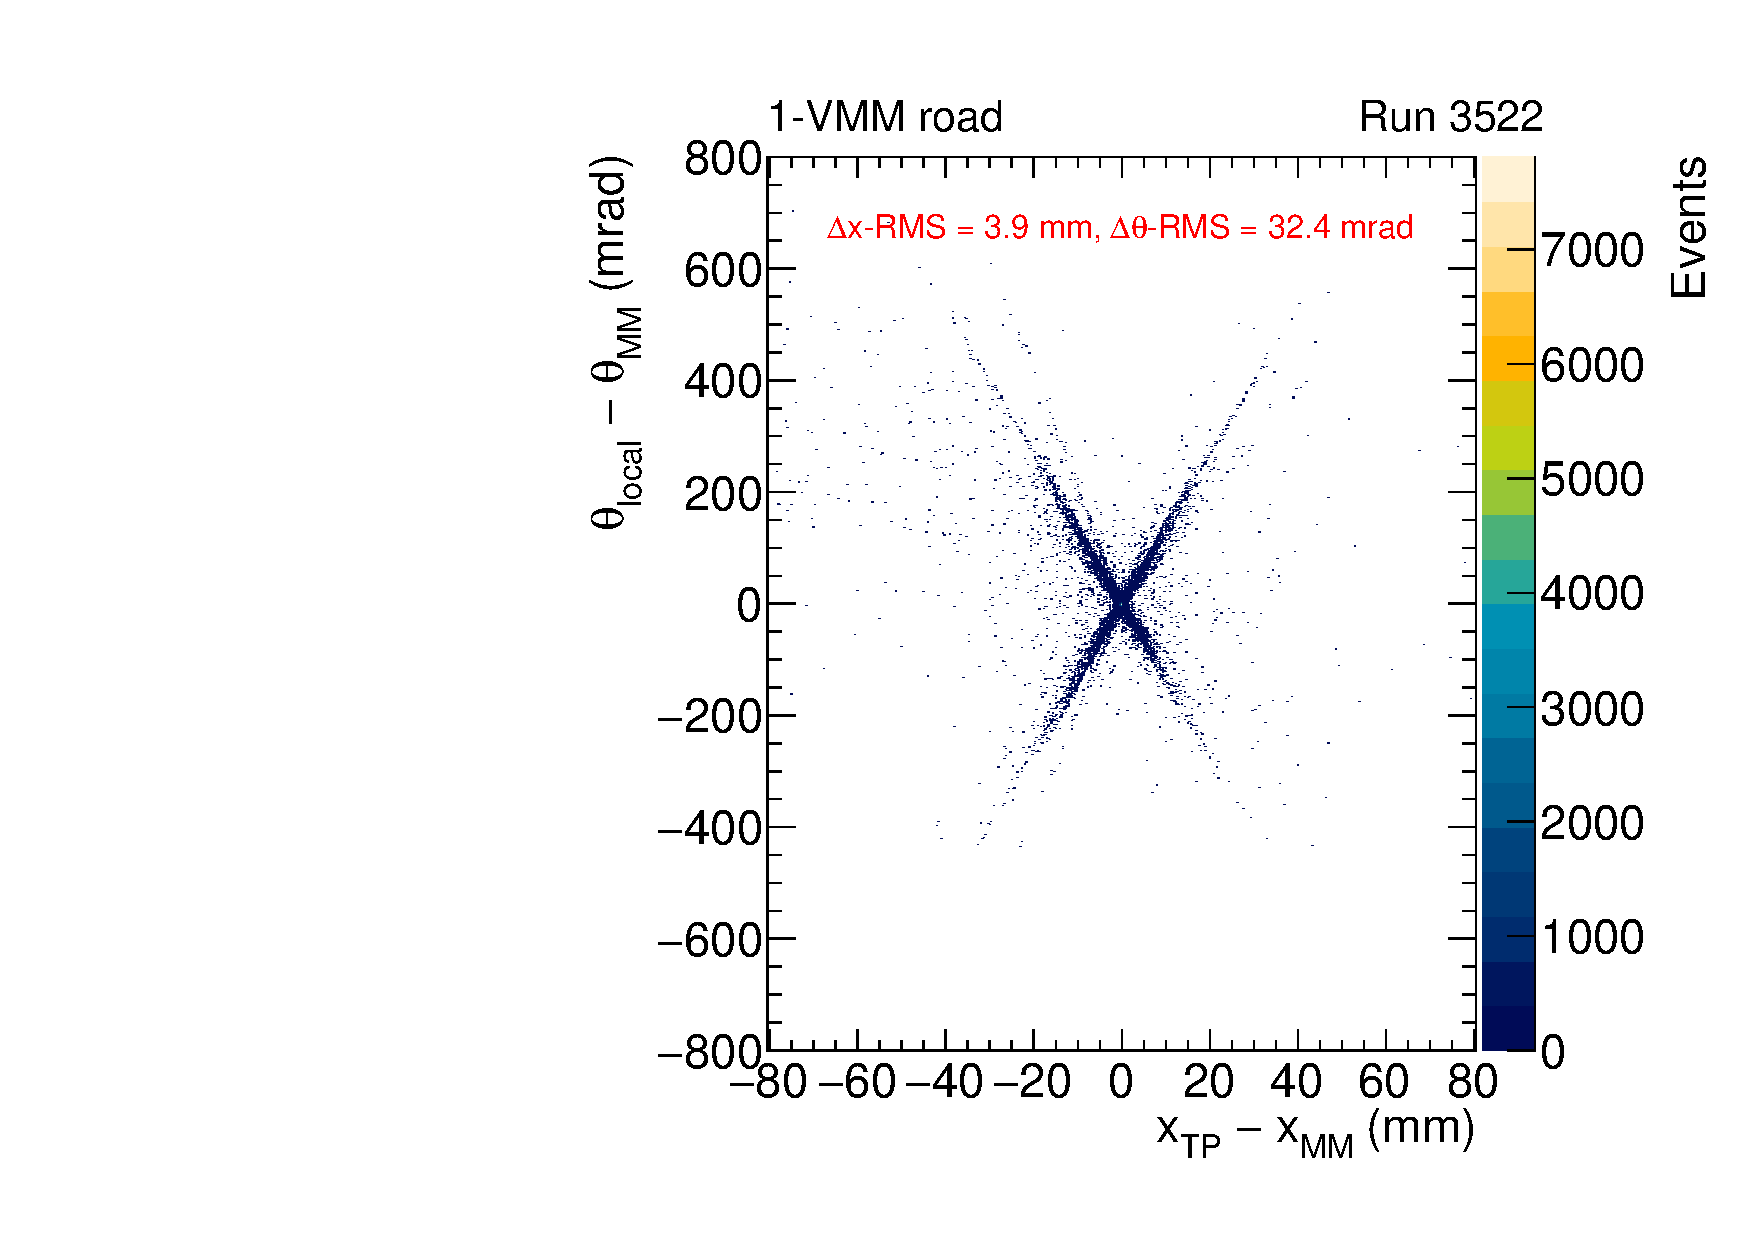
\includegraphics[width=0.48\textwidth]{figures/gbtanalysis3522/TP_xres_angres_full.pdf}
    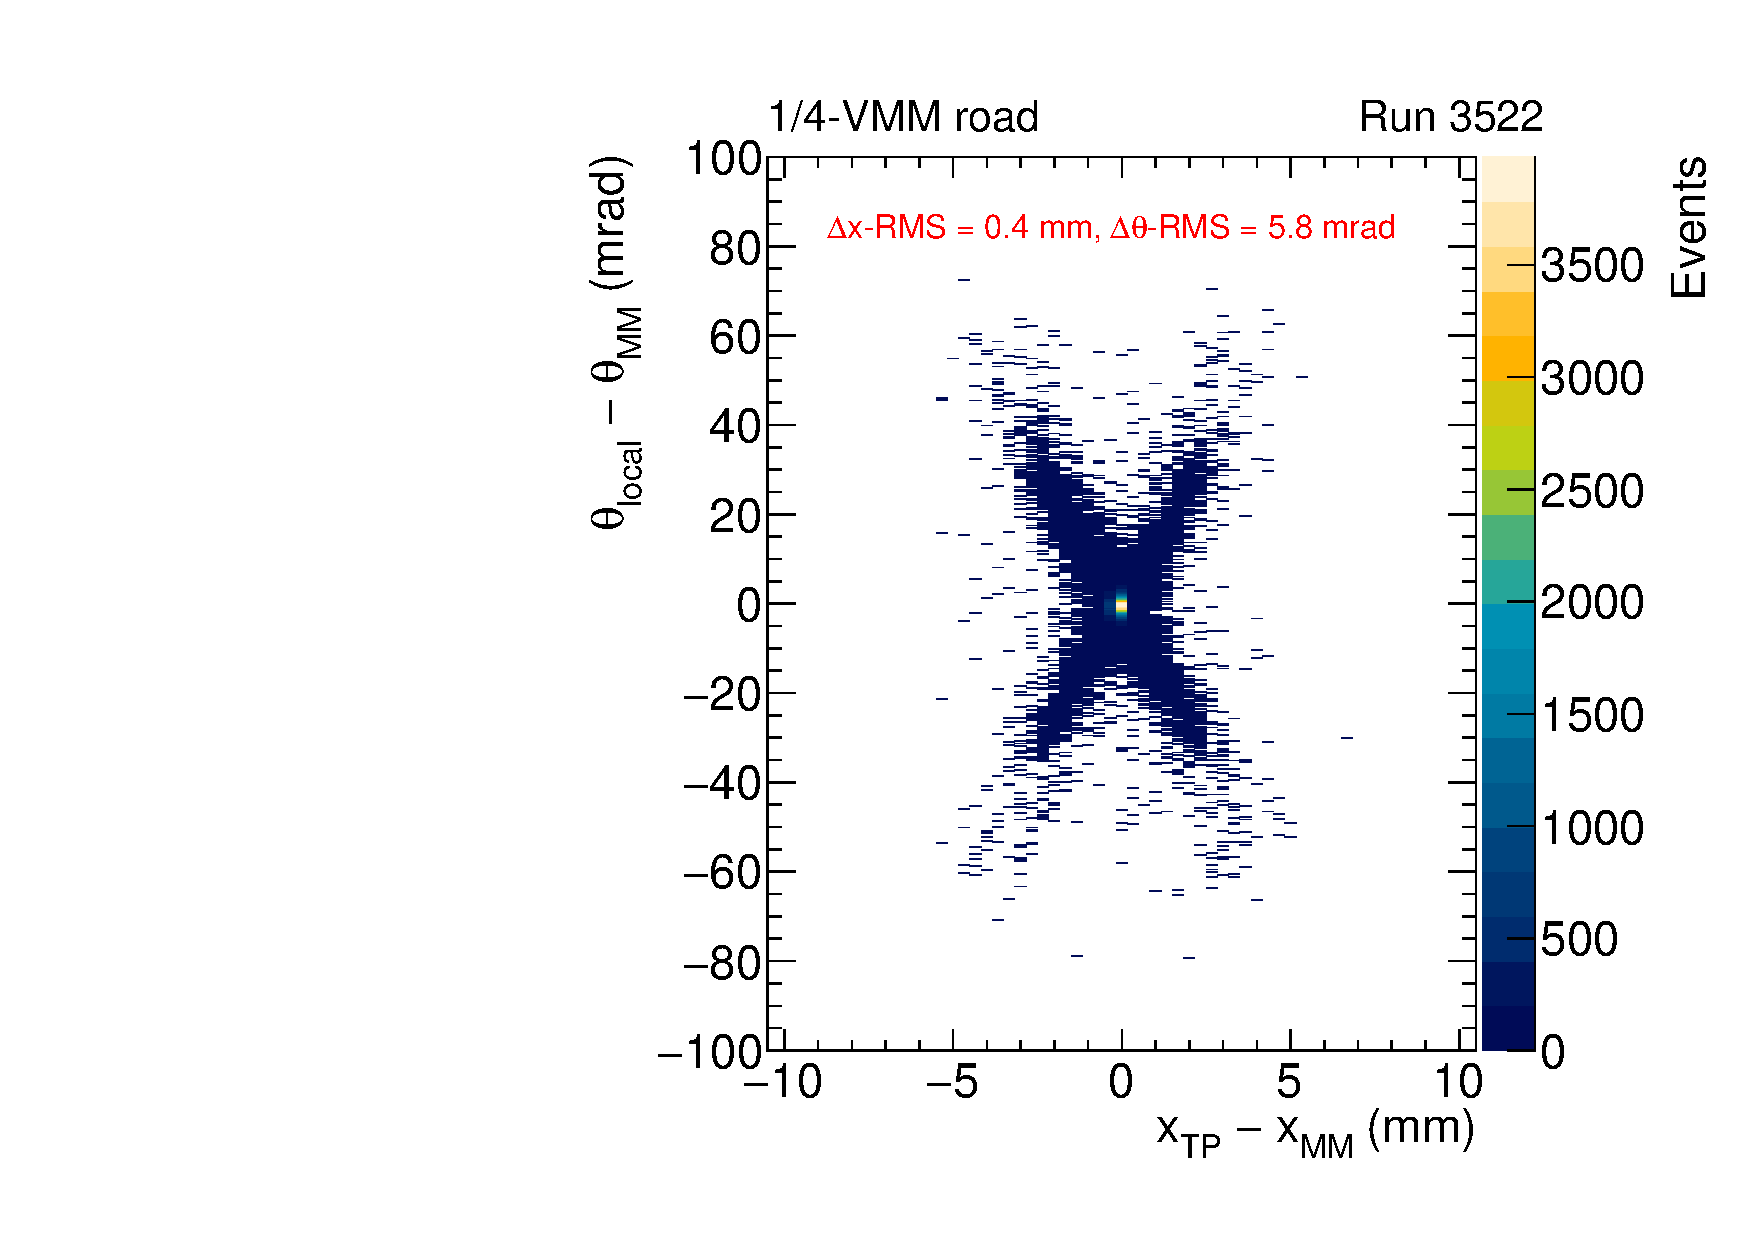
\includegraphics[width=0.48\textwidth]{figures/gbtanalysis3522/TP_xres_angres.pdf}
  \end{center}
  \vspace{-10pt}
  \caption{The $x$ and $\theta$ resolution of the MMTP relative to the full readout, using 1-VMM online roads (left) and 1/4-VMM offline roads (right), as discussed in Section~\ref{sec:perf-roads}. The tails of the resolution are greatly suppressed with smaller roads.}
  \label{fig:xthetares}
\end{figure}

\subsection{Time resolution}

The time resolution measured with cosmic data is shown in two ways. First, the timing of ART hits within a trigger are compared against themselves. Second, the timing is compared against the scintillator timestamp as a reference.

As discussed in Section~\ref{sec:alg-finder}, the MMTP algorithm here collects ART hits in a window of 7 BCs. The measured \textit{BC window} per trigger is then defined as the number of BCs the algorithm actually needed to collect all the hits for a given trigger. For example, if all hits arrive at the same BC, the BC window is 1.

Additionally, the time resolution of individual hits is measured by choosing all possible pairs of hits within a trigger and measuring the difference in their BCIDs. The resolution of this quantity is then related to the time resolution of individual hits by $\sigma(t_i - t_j) = \sqrt{2}\ \sigma(t)$.

These distributions are shown in Figure~\ref{fig:time}. The measured time resolution is worse than what is reported in the TDR. Simulation of the Micromegas in the NSW have suggested a BC window of 2 BCs would be sufficient to collect trigger hits with better than 99\% efficiency~\cite{koki}. The measurements here indicate a window of 5-10 BCs is more likely needed to achieve a good efficiency. The distribution of $\Delta BC$ for pairs of ART hits gives a fitted $\sigma$ of 2.15 BCs, corresponding to a time resolution of 38 ns per hit.

\begin{figure}[!htpb]
  \begin{center}
    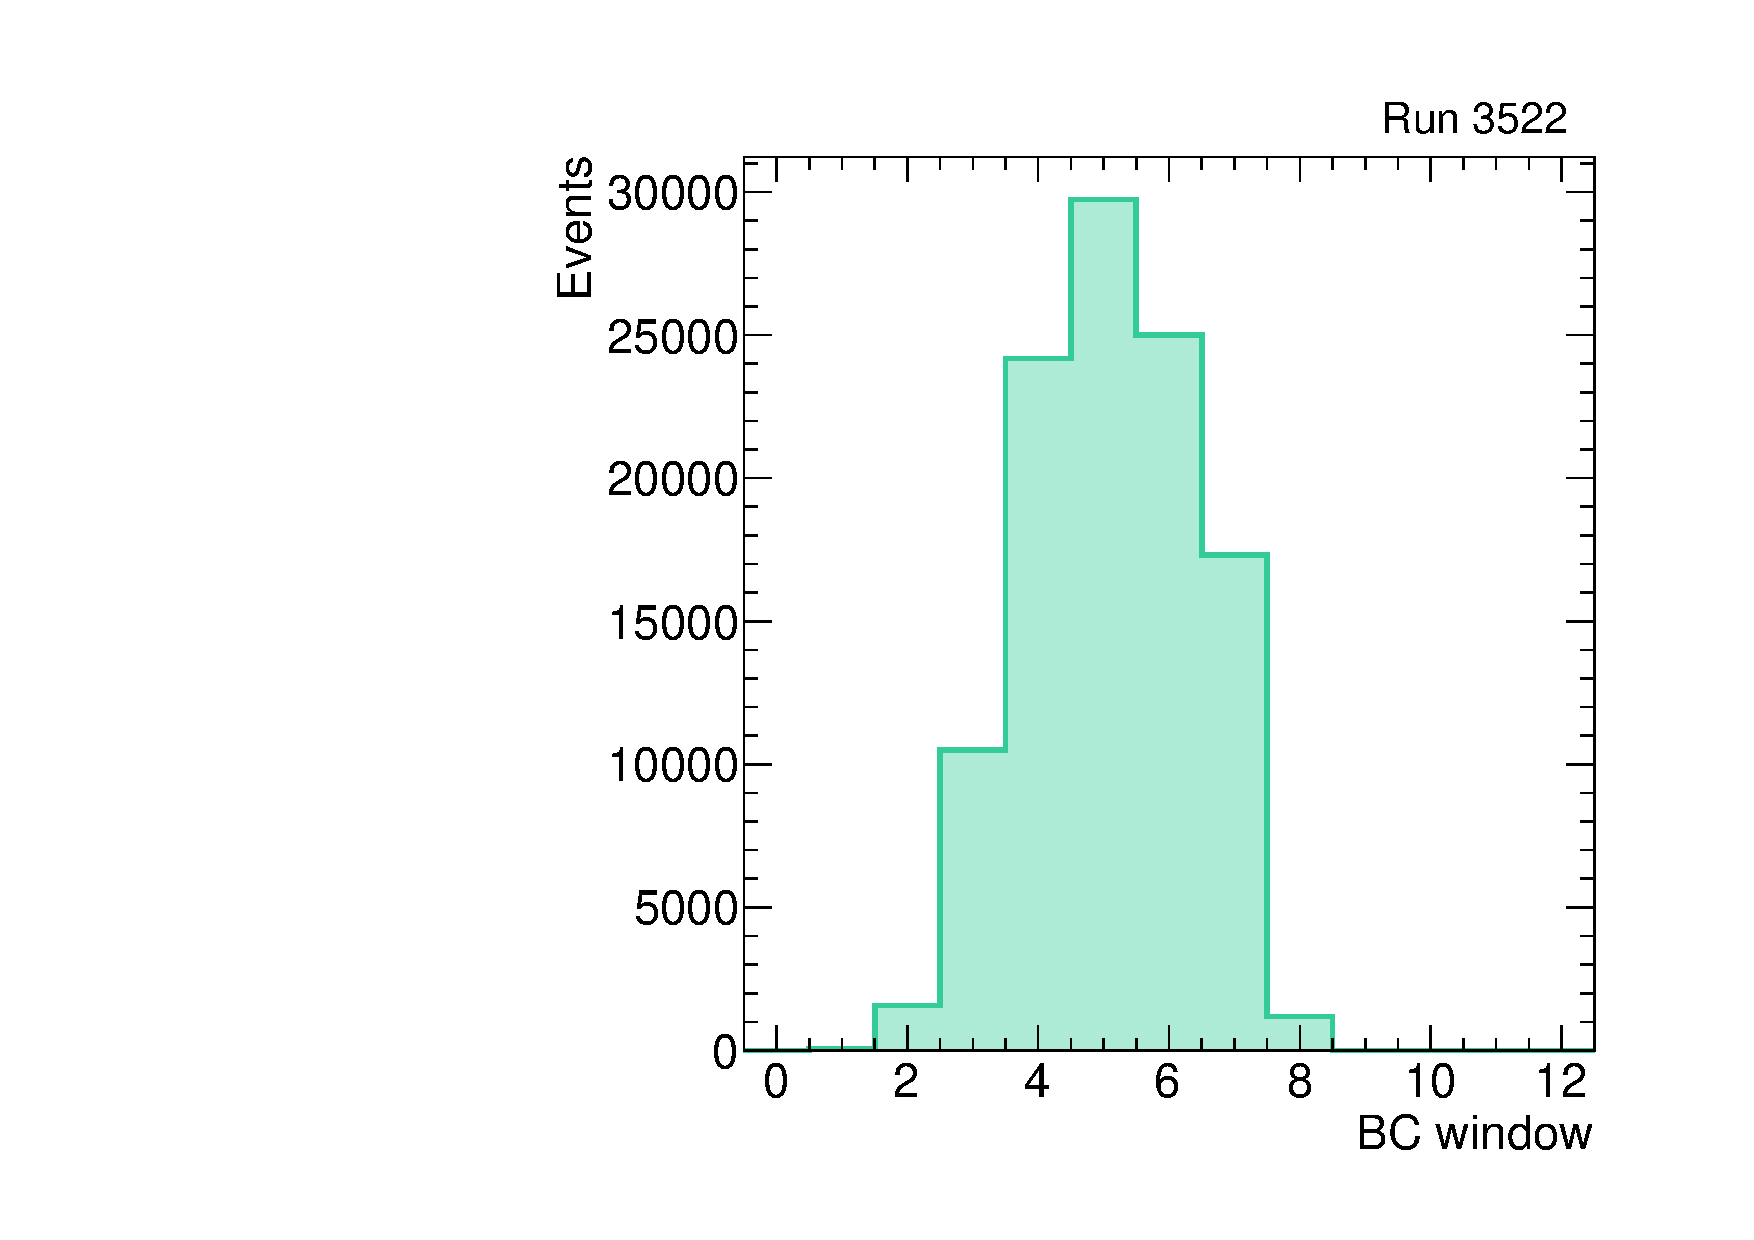
\includegraphics[width=0.48\textwidth]{figures/gbtanalysis3522/artwin_lin.pdf}
    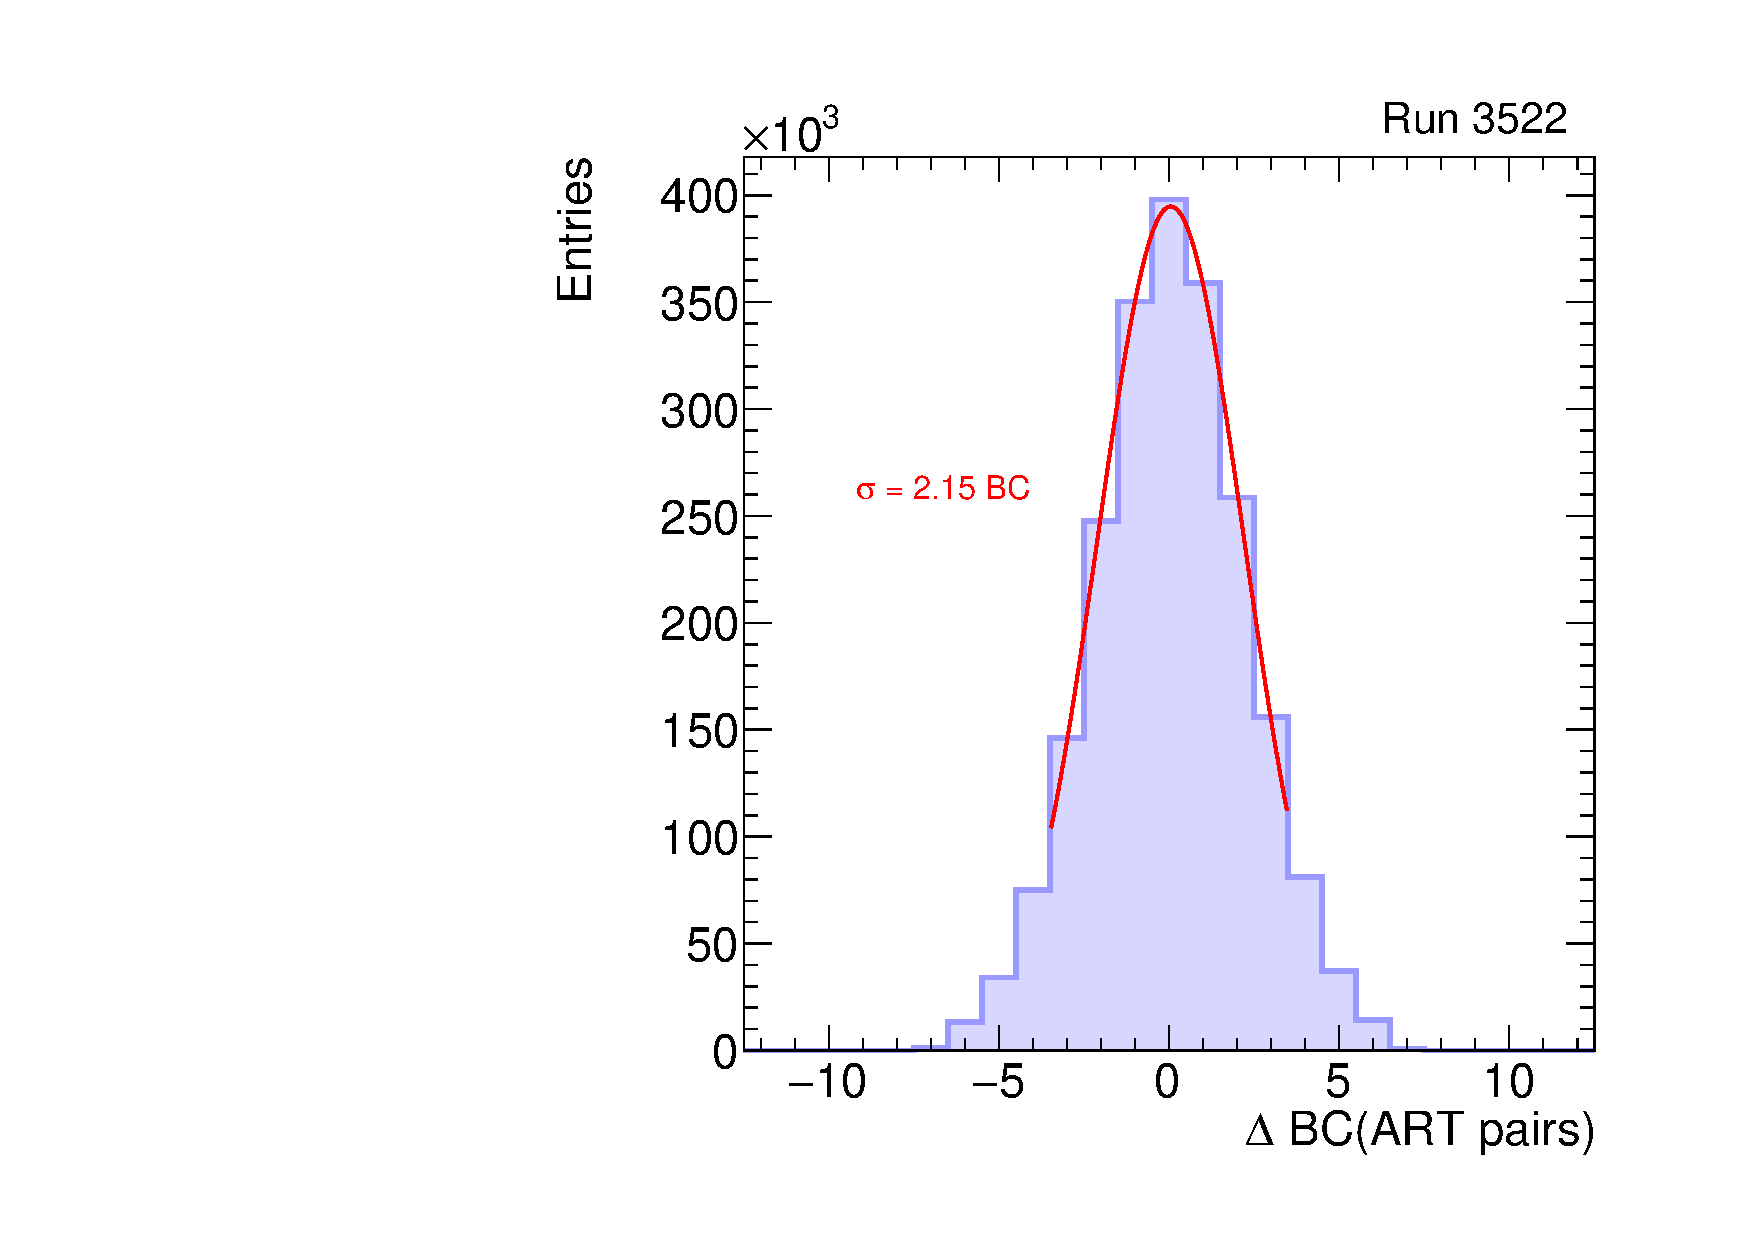
\includegraphics[width=0.48\textwidth]{figures/gbtanalysis3522/artrpairs_lin.pdf}
  \end{center}
  \vspace{-10pt}
  \caption{The time window required to record all hits in a trigger (left) and the $\Delta\text{BC}$ of all pairs of hits in a trigger (right). A gaussian fit is overlaid on the distribution of $\Delta\text{BC}$ and describes the data well.}
  \label{fig:time}
\end{figure}

A global time measurement per trigger is also of interest for the NSW. This is needed to match tracks found in the NSW with tracks found by the TGCs in the big wheel. It will be one of the parameters sent to downstream clients of the NSW trigger, along with the position and quality of a trigger.

A per-trigger time resolution is measured with cosmic data by comparing the time of hits within the trigger to the time reported by the scintillator, which has a resolution of 1-2 ns after being processed by the MMTP FPGA. Two methods are considered for making a trigger-level BCID: the average BCID of all hits, and the earliest BCID of all hits. The distributions are shown in Figure~\ref{fig:timeres}. The average BCID agrees with the reference BCID with $\sim\!50\%$ efficiency, and the earliest BCID agrees with reference with $\sim\!41\%$ efficiency.

\begin{figure}[!htpb]
  \begin{center}
    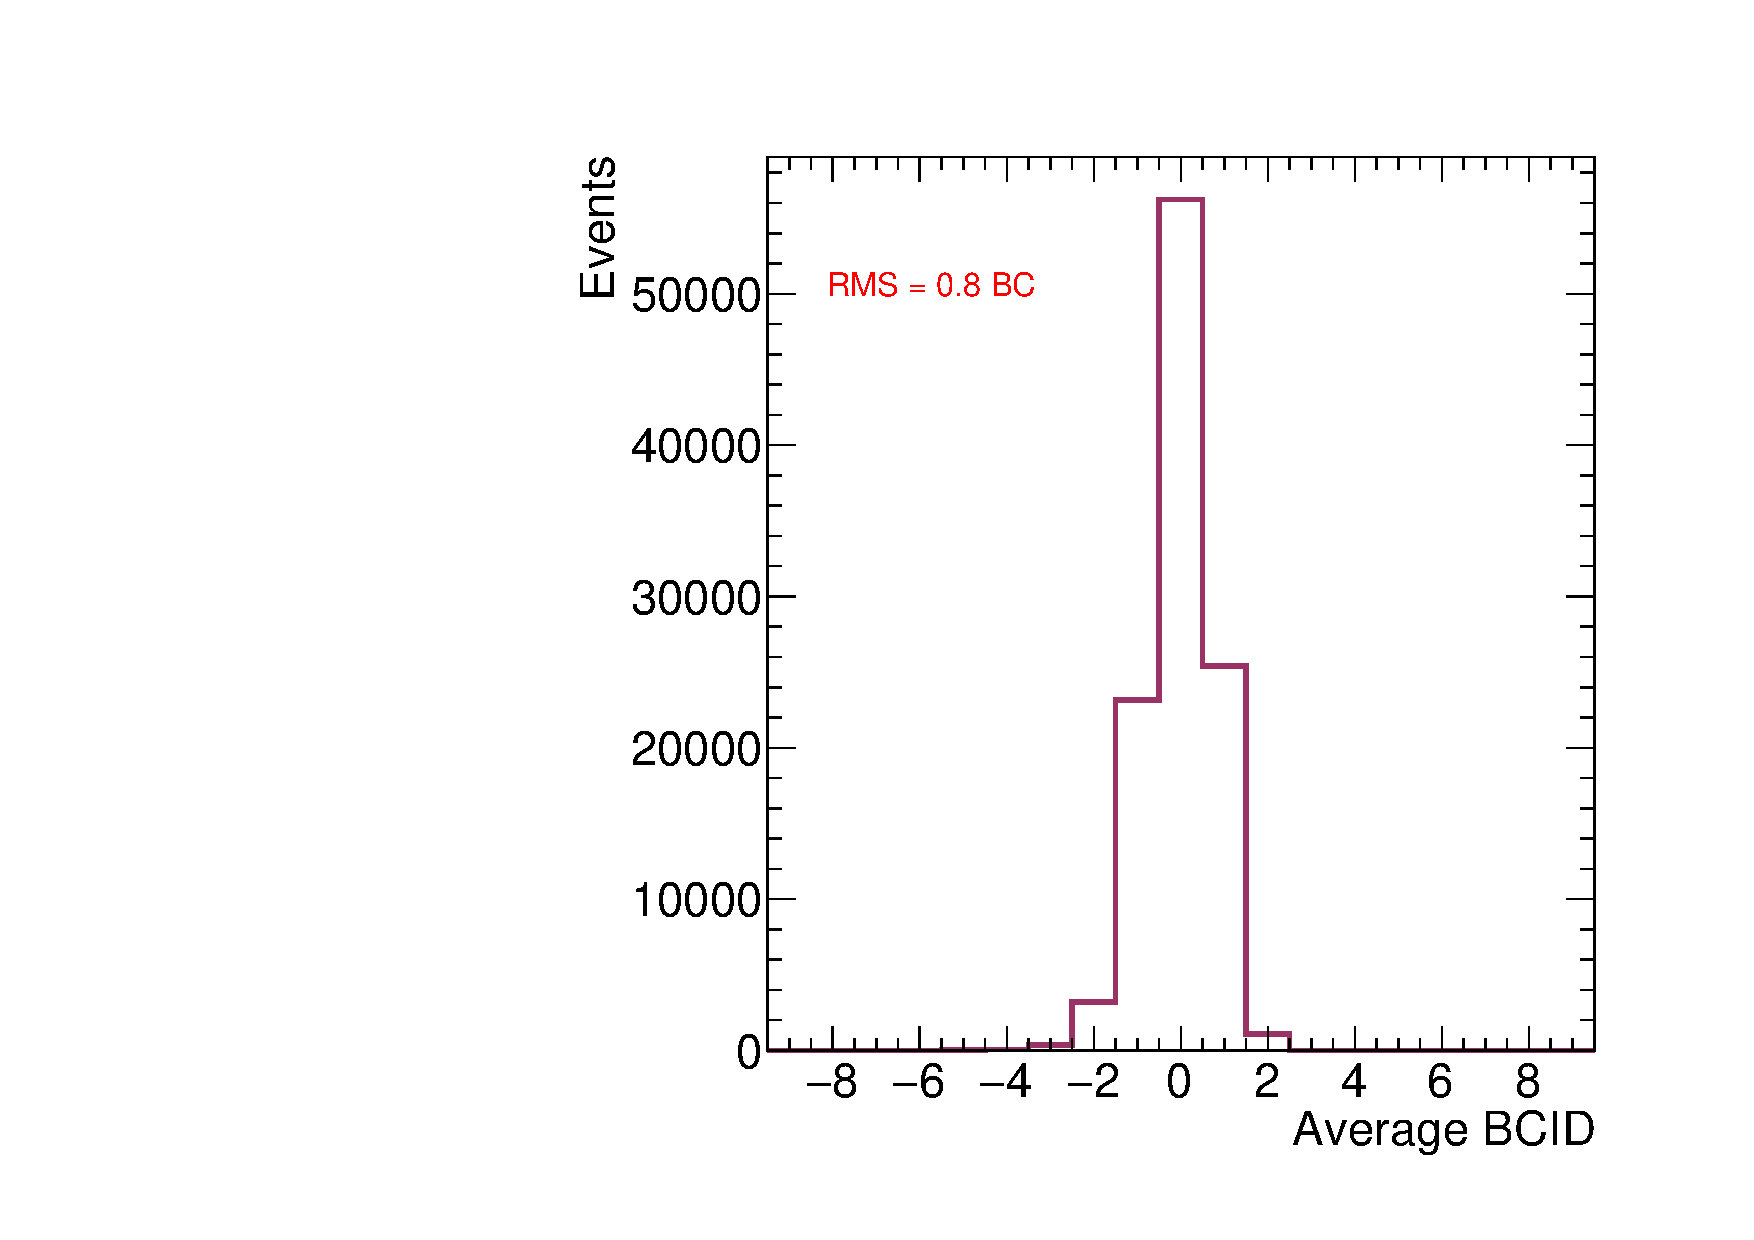
\includegraphics[width=0.48\textwidth]{figures/gbtanalysis3522/avg_BCID.pdf}
    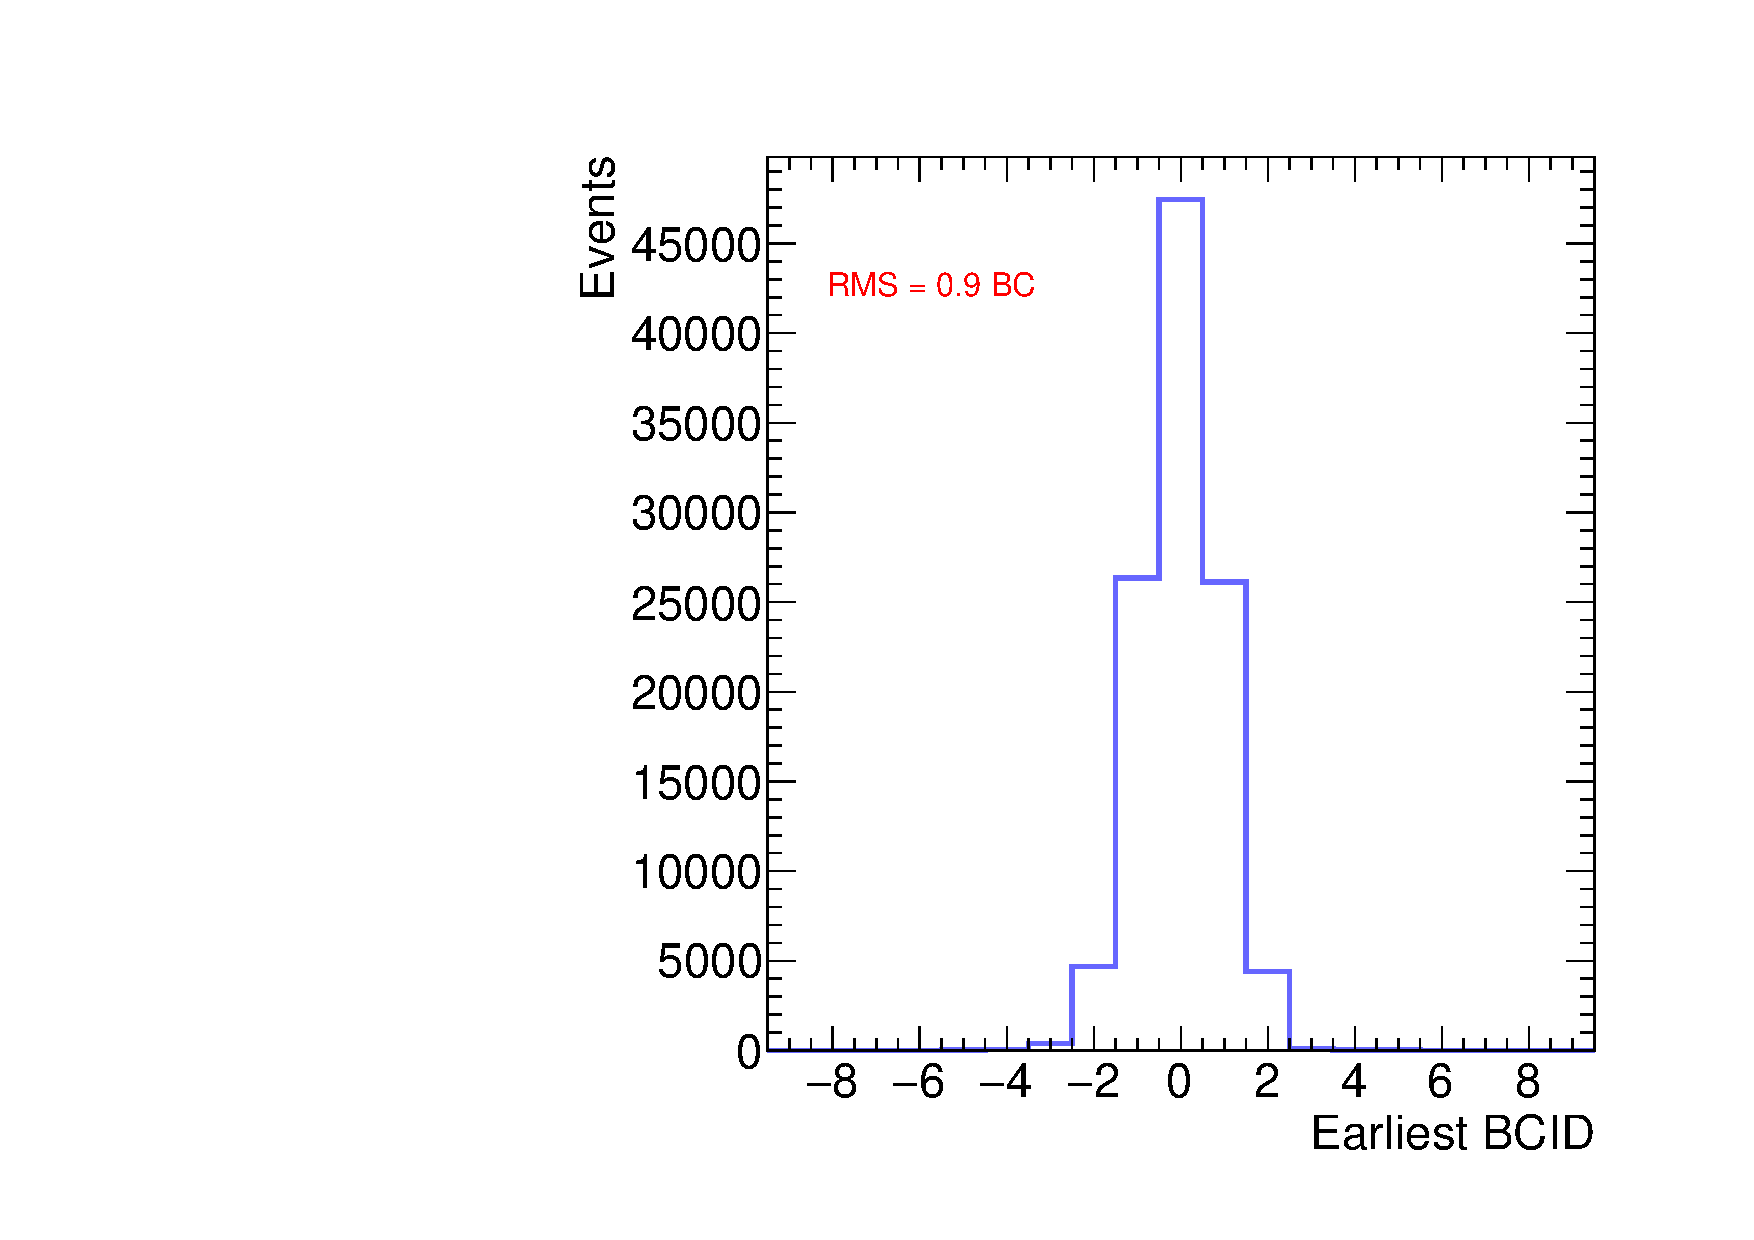
\includegraphics[width=0.48\textwidth]{figures/gbtanalysis3522/earliest_BCID.pdf}
  \end{center}
  \vspace{-10pt}
  \caption{The time resolution of the MMTP relative to the scintillator. The BCID of the trigger can be defined as the average BCID of the ART hits (left) or the earliest BCID (right). Choosing the average BCID performs better than choosing the earliest.}
  \label{fig:timeres}
\end{figure}

\subsection{Integration time}
\label{sec:perf-integ}

The performance of the MMTP is also considered for different integration times of the front-end VMM2 chip. The integration times considered are 200 ns, 100 ns, and 50 ns. The results presented elsewhere in the section are exclusively with 200 ns integration time.

The efficiency, spatial resolution, and angular resolution are found to not depend significantly on the integration time. They are shown in Appendex~\ref{}. The time resolution of ART hits and the trigger improve with smaller integration time, as shown in Figures~\ref{fig:integ_window},~\ref{fig:integ_pairs},~\ref{fig:integ_avg_bc}, and~\ref{fig:integ_avg_earliest}. Specifically, the time resolution of individual hits decreases from 40 ns to 32 ns when shortening the integration time from 200 ns to 50 ns.

Operating the NSW with short integration then presents one option for improving the time resolution of the Micromegas trigger. However, we note the Micromegas detectors used in this note were operated with a high voltage of 560-570 V, near the maximum voltage. At lower voltage, the efficiency loss of shorter integration time would become a more significant factor.

\begin{figure}[!htpb]
  \begin{center}
    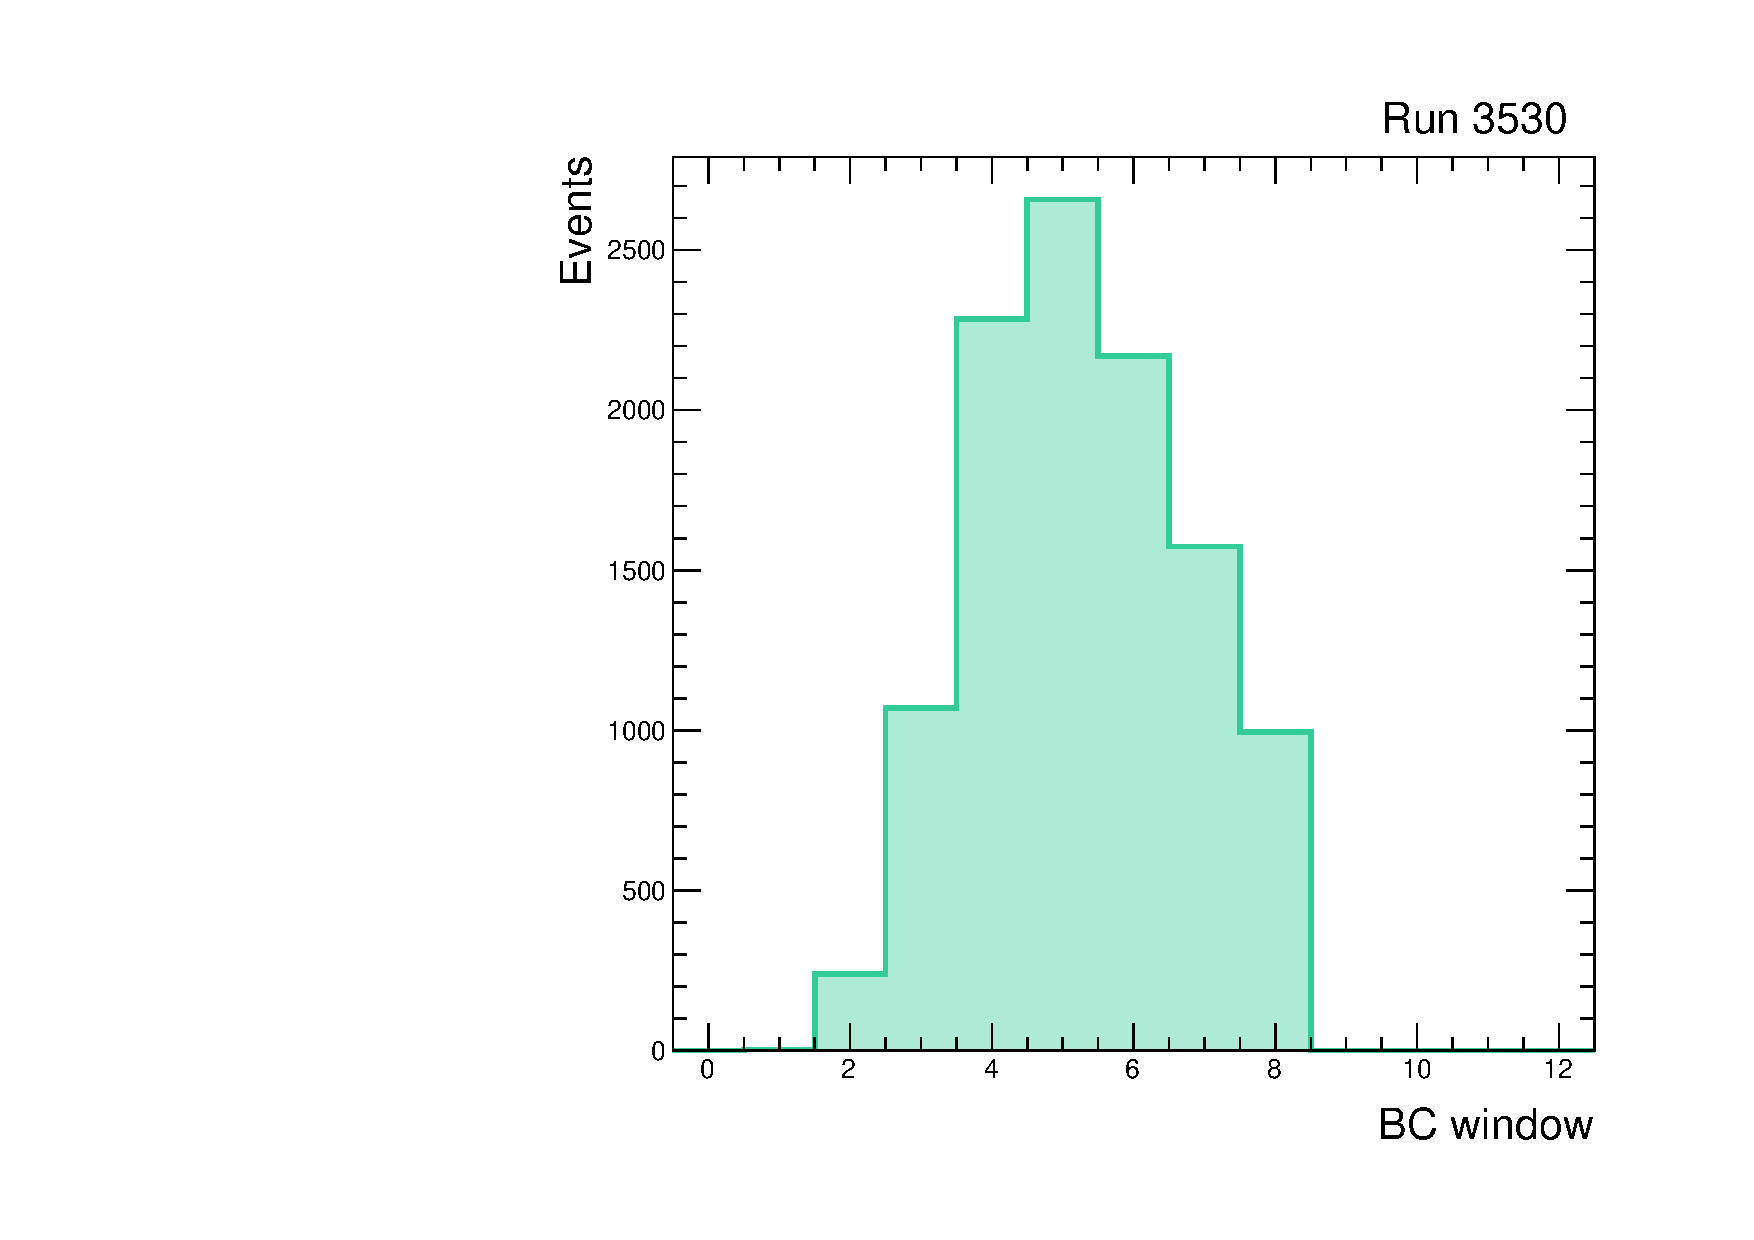
\includegraphics[width=0.3\textwidth]{figures/gbtanalysis3530/artwin_lin.pdf}
    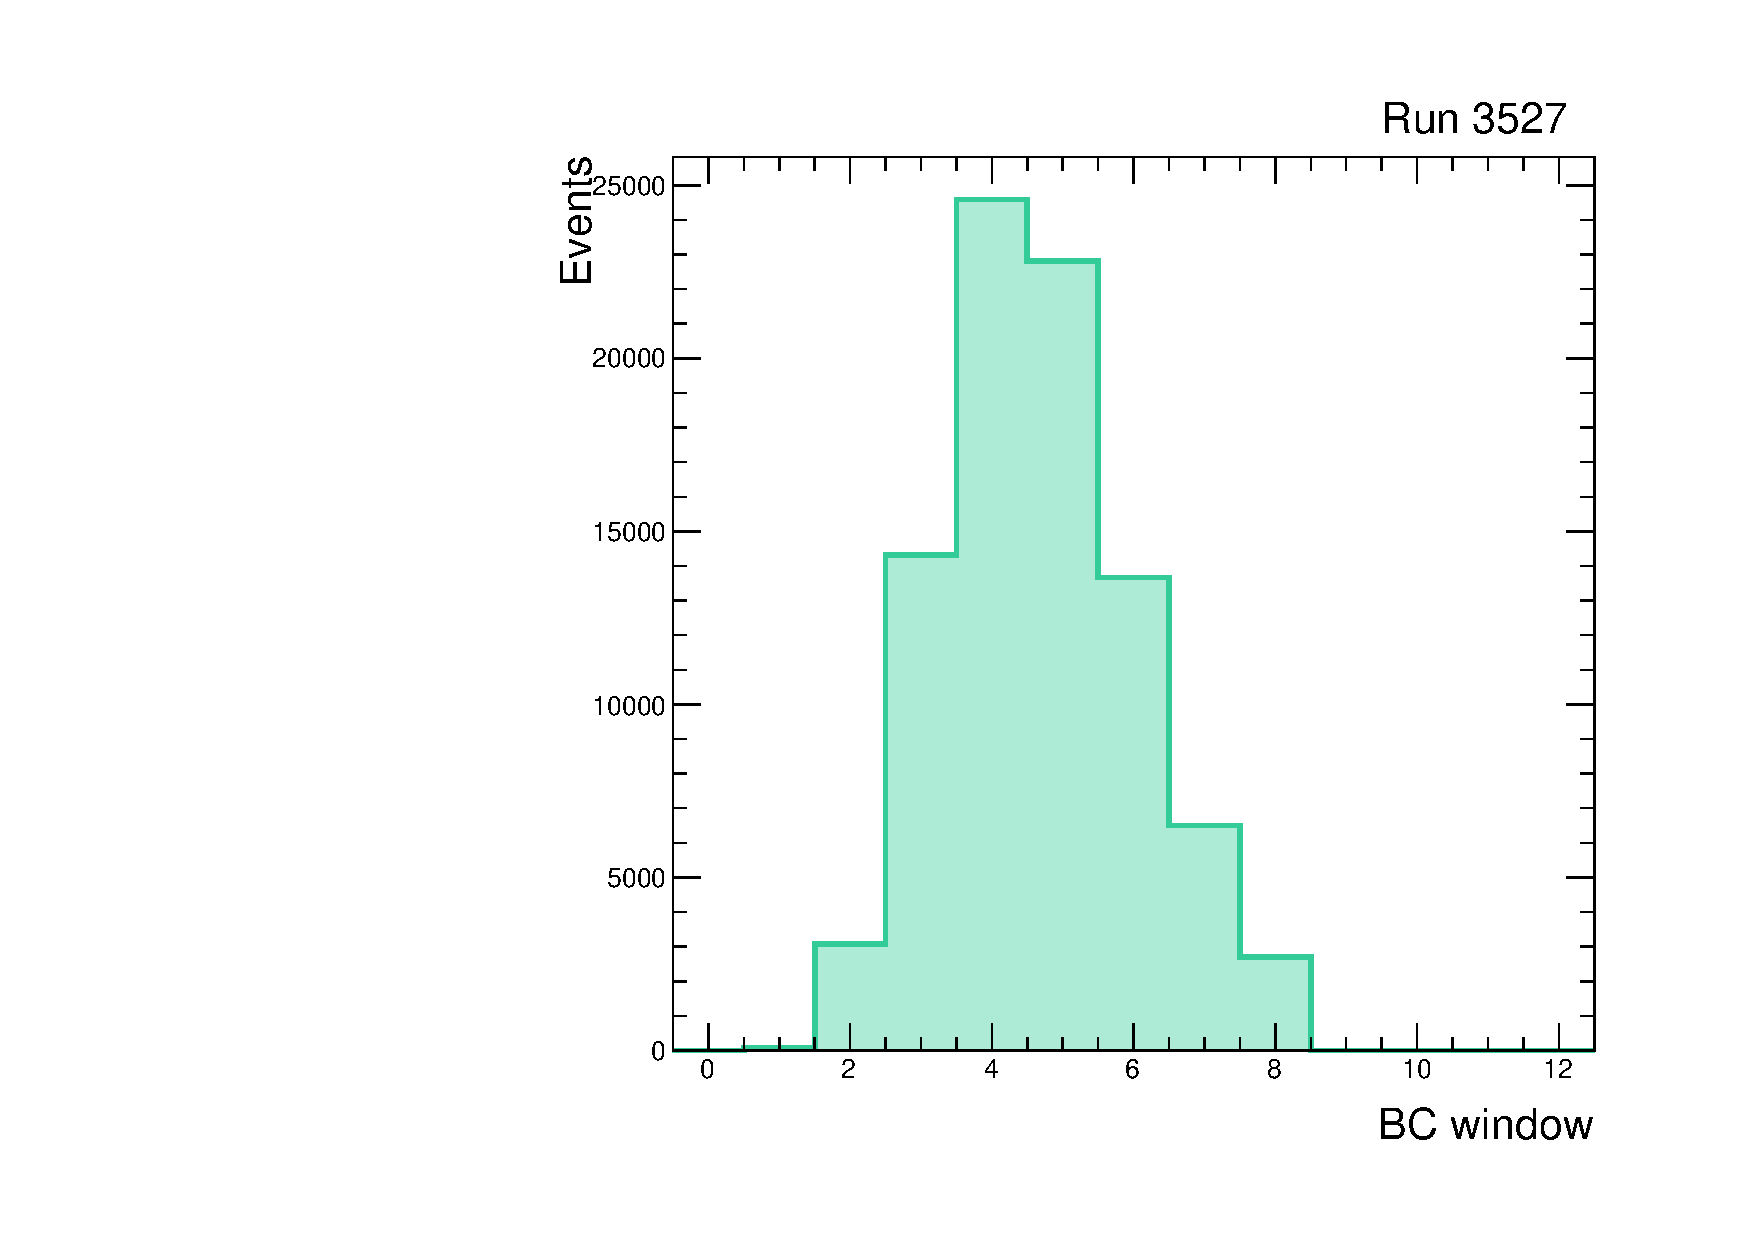
\includegraphics[width=0.3\textwidth]{figures/gbtanalysis3527/artwin_lin.pdf}
    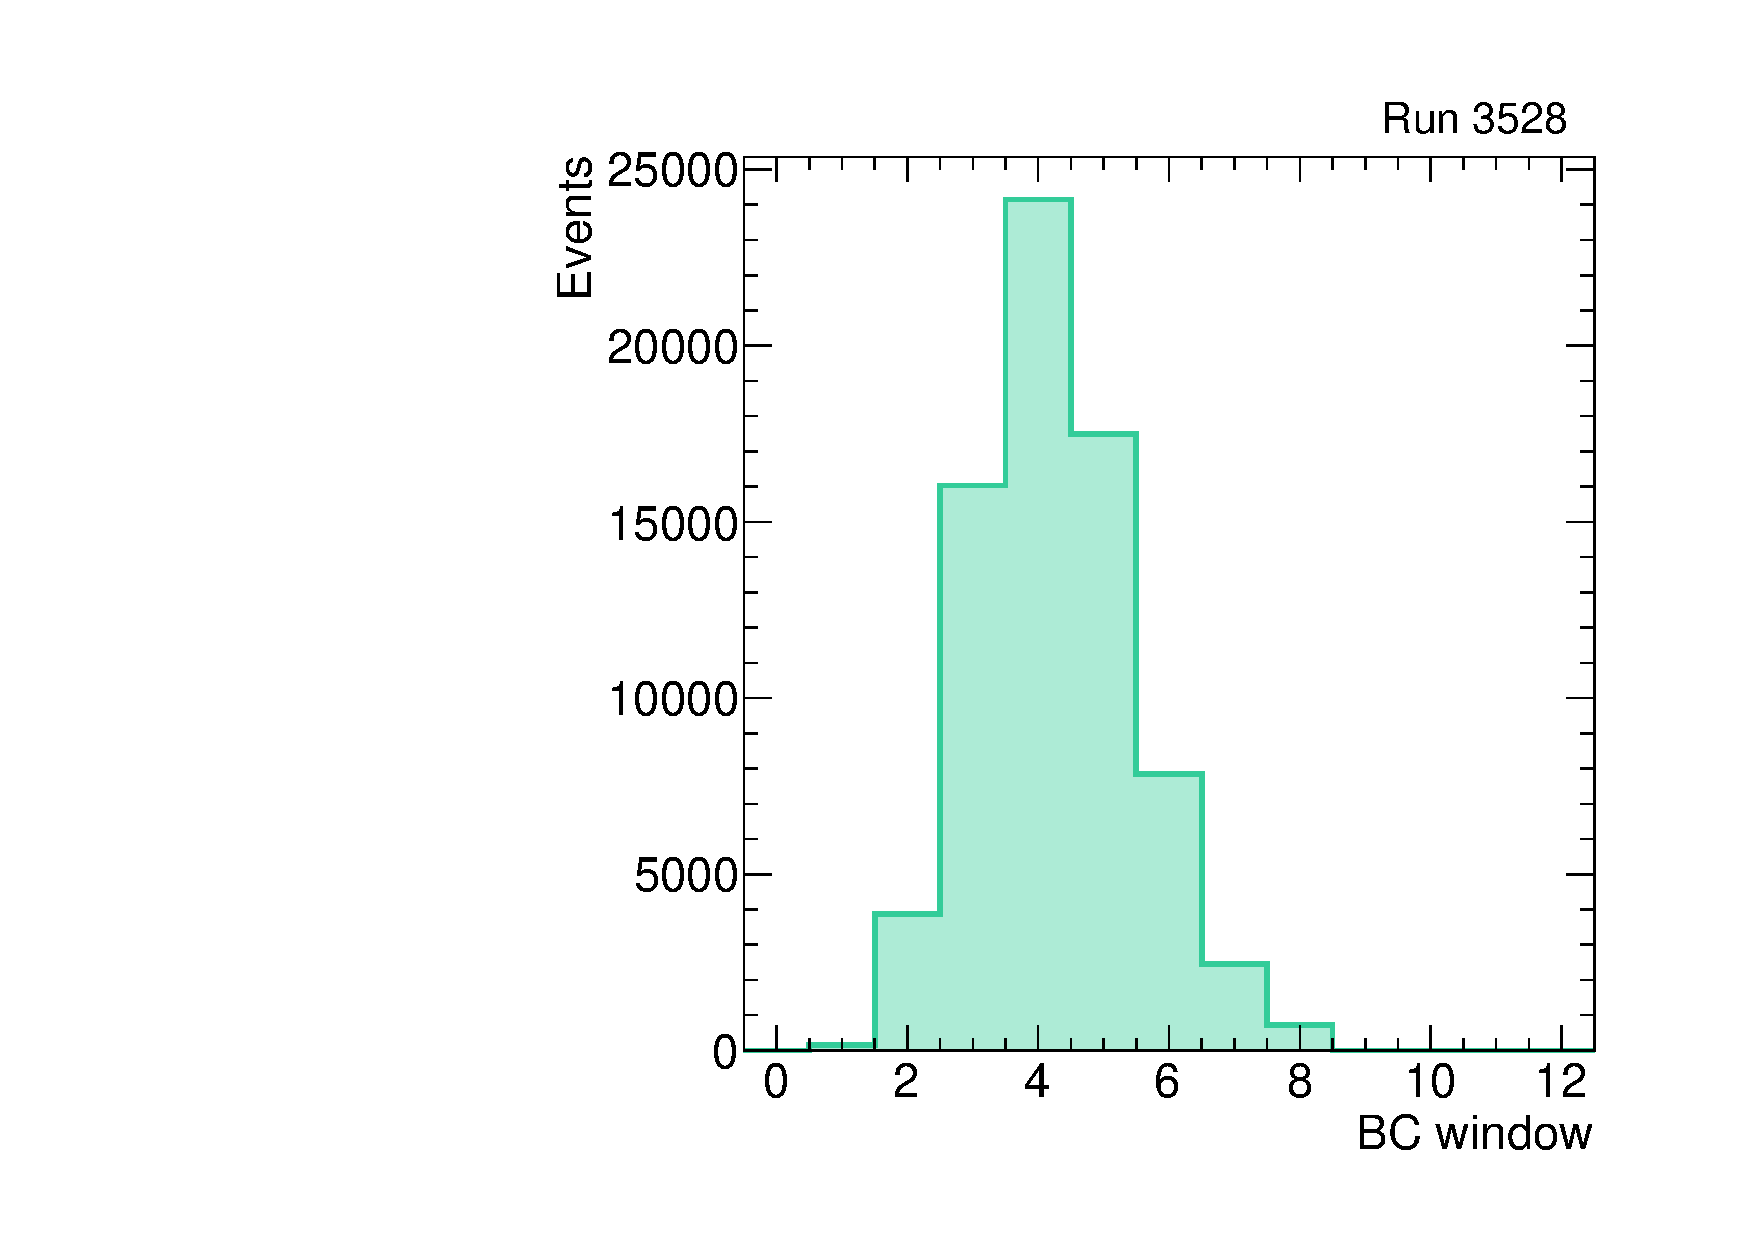
\includegraphics[width=0.3\textwidth]{figures/gbtanalysis3528/artwin_lin.pdf}
  \end{center}
  \vspace{-10pt}
  \caption{The time window required to record all hits in a trigger for data collected with 200 ns (left), 100 ns (middle), and 50 ns (right) integration time in the VMM. The window decreases as the integration time decreases.}
  \label{fig:integ_window}
\end{figure}

\begin{figure}[!htpb]
  \begin{center}
    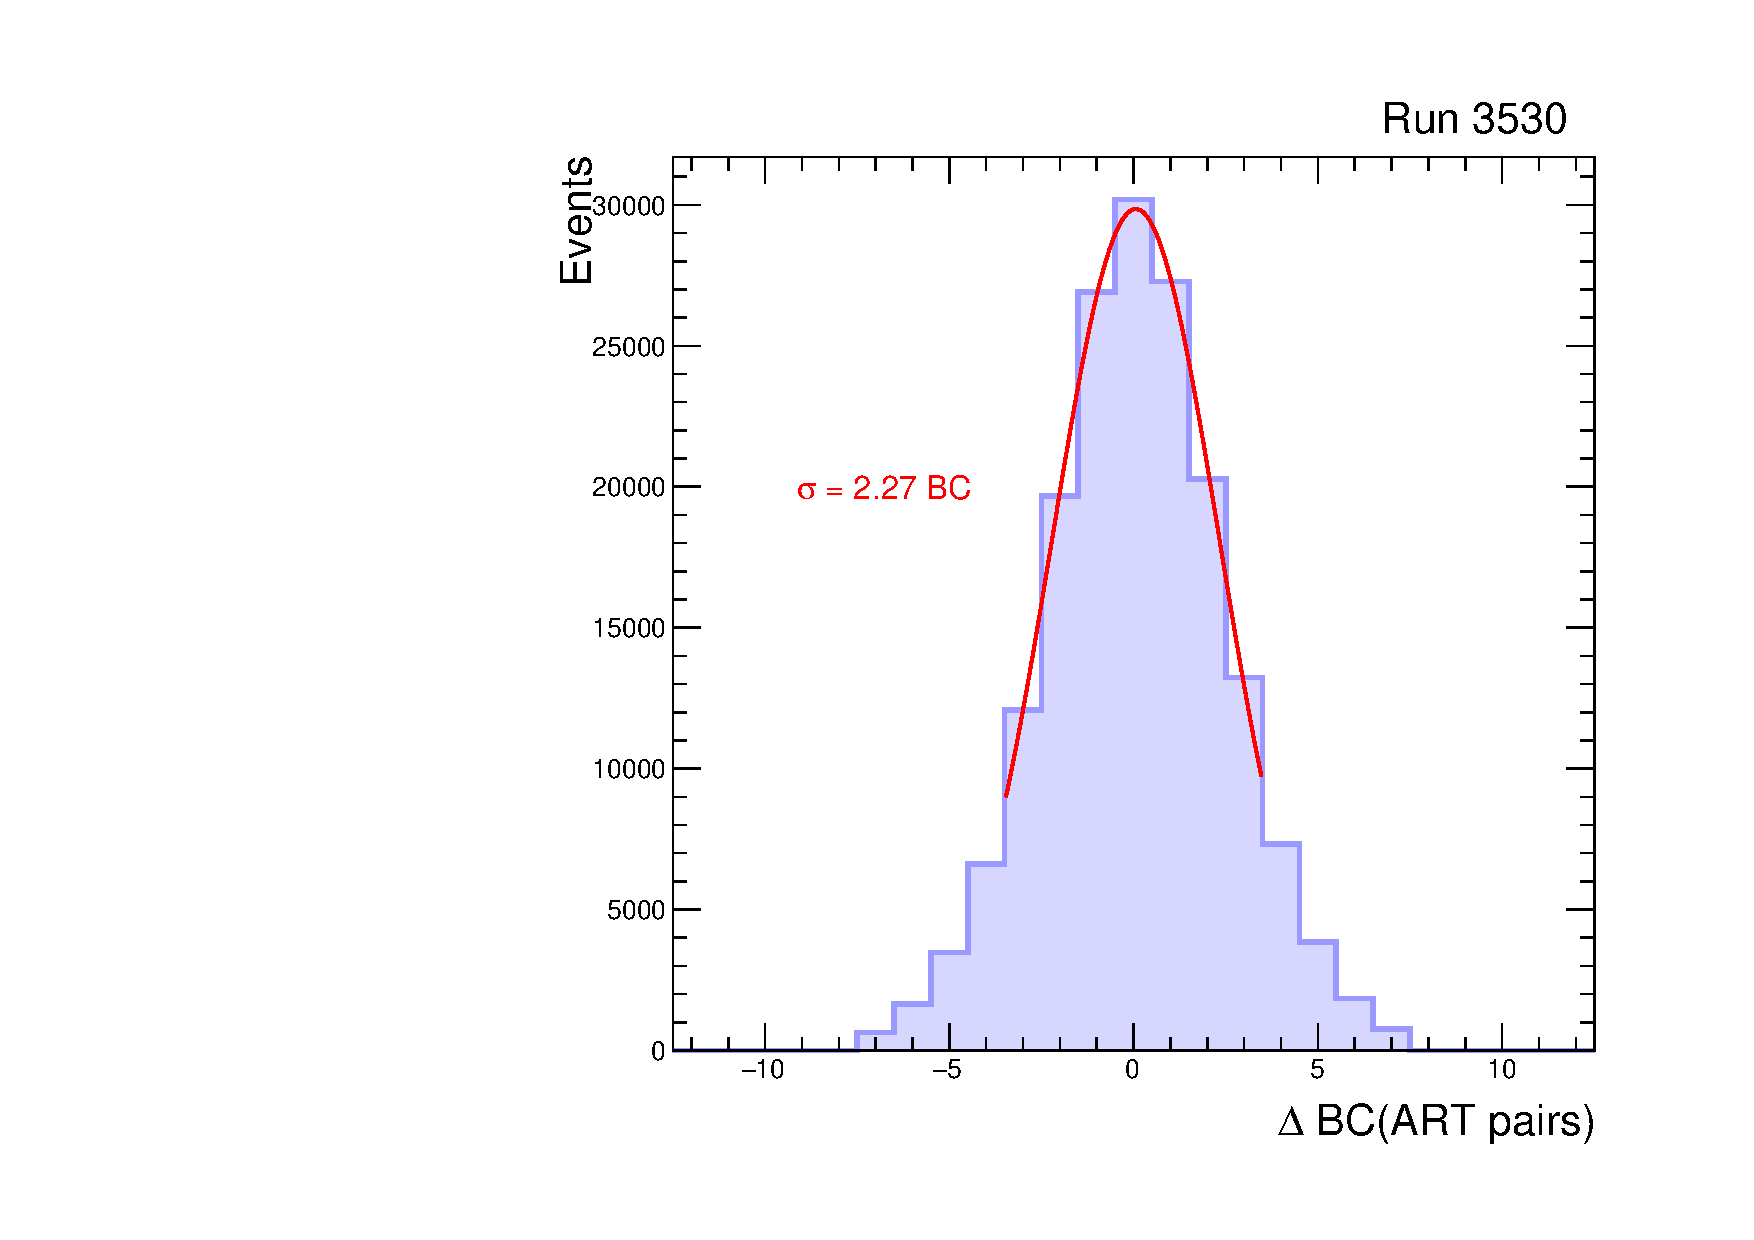
\includegraphics[width=0.3\textwidth]{figures/gbtanalysis3530/artrpairs_lin.pdf}
    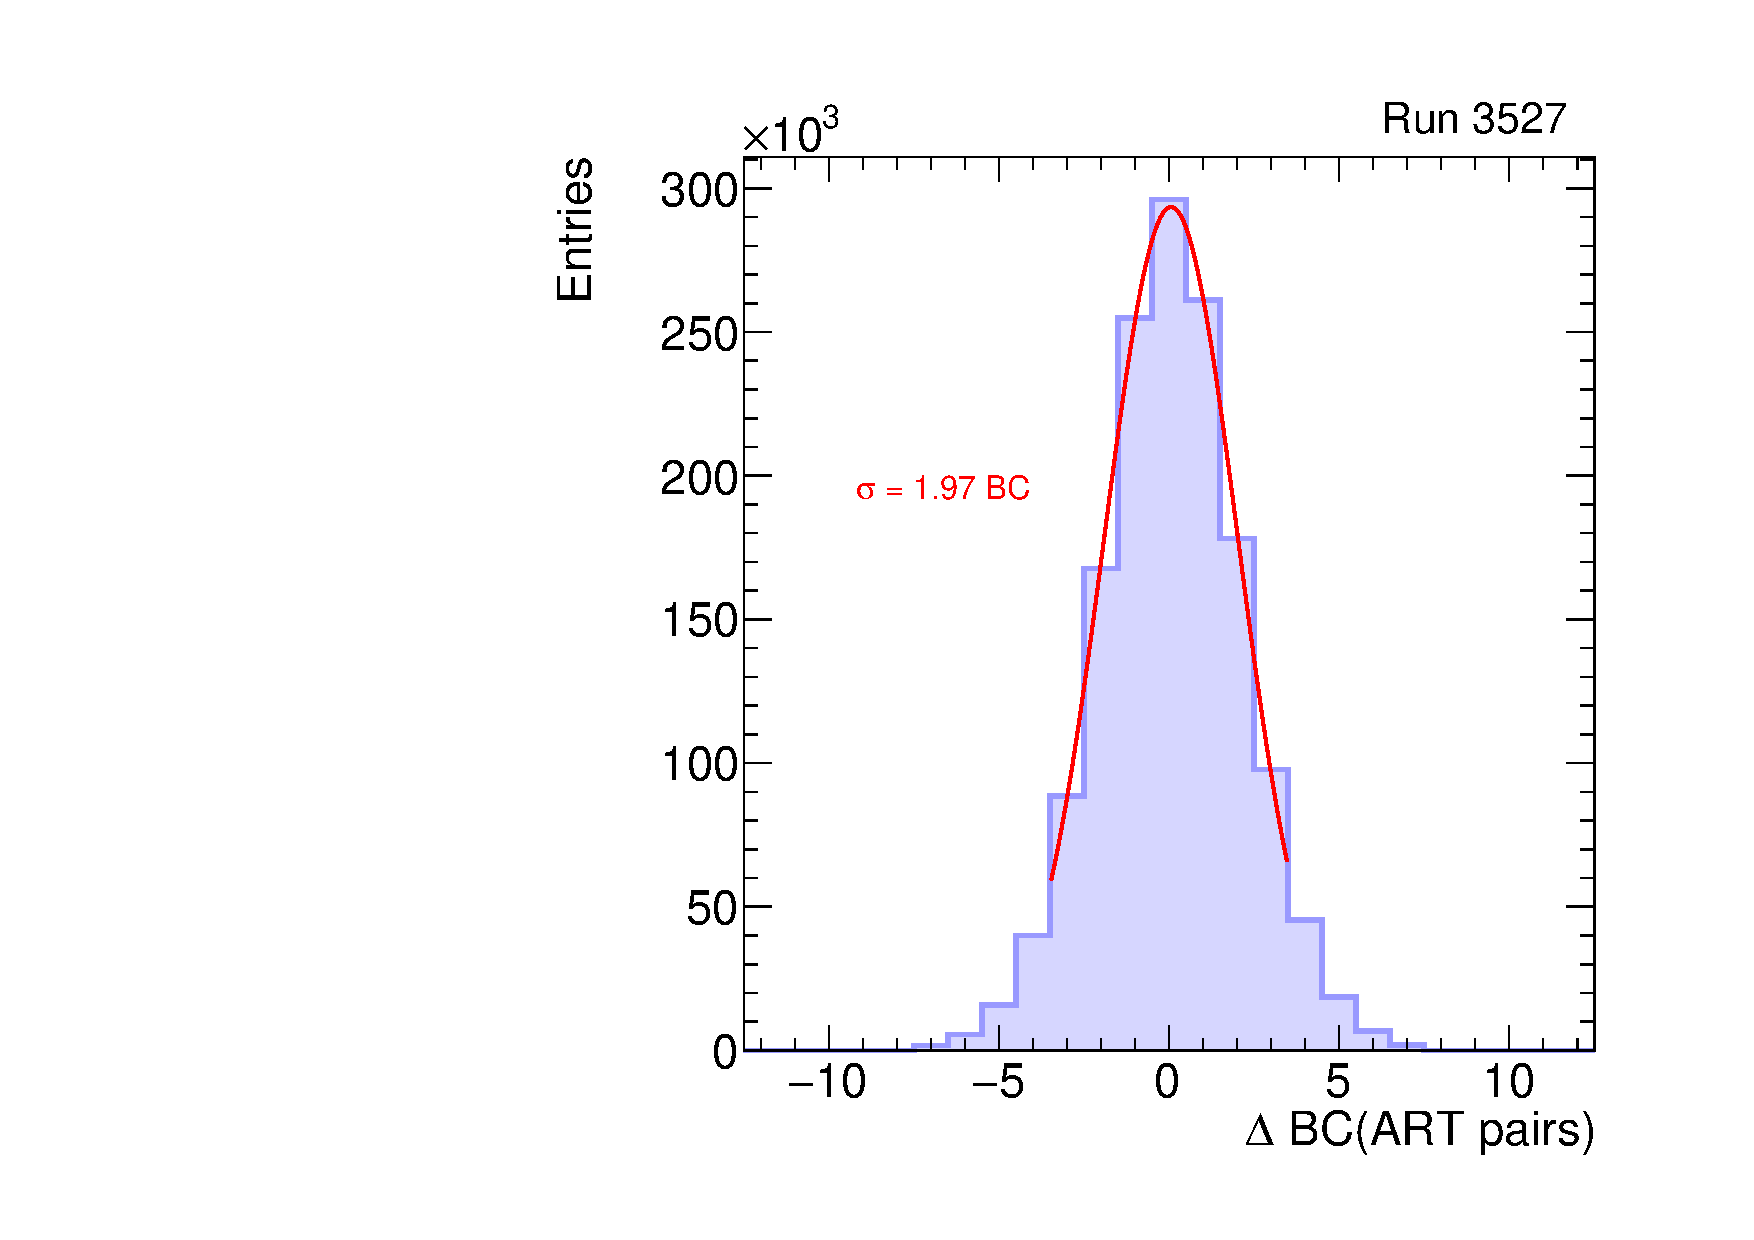
\includegraphics[width=0.3\textwidth]{figures/gbtanalysis3527/artrpairs_lin.pdf}
    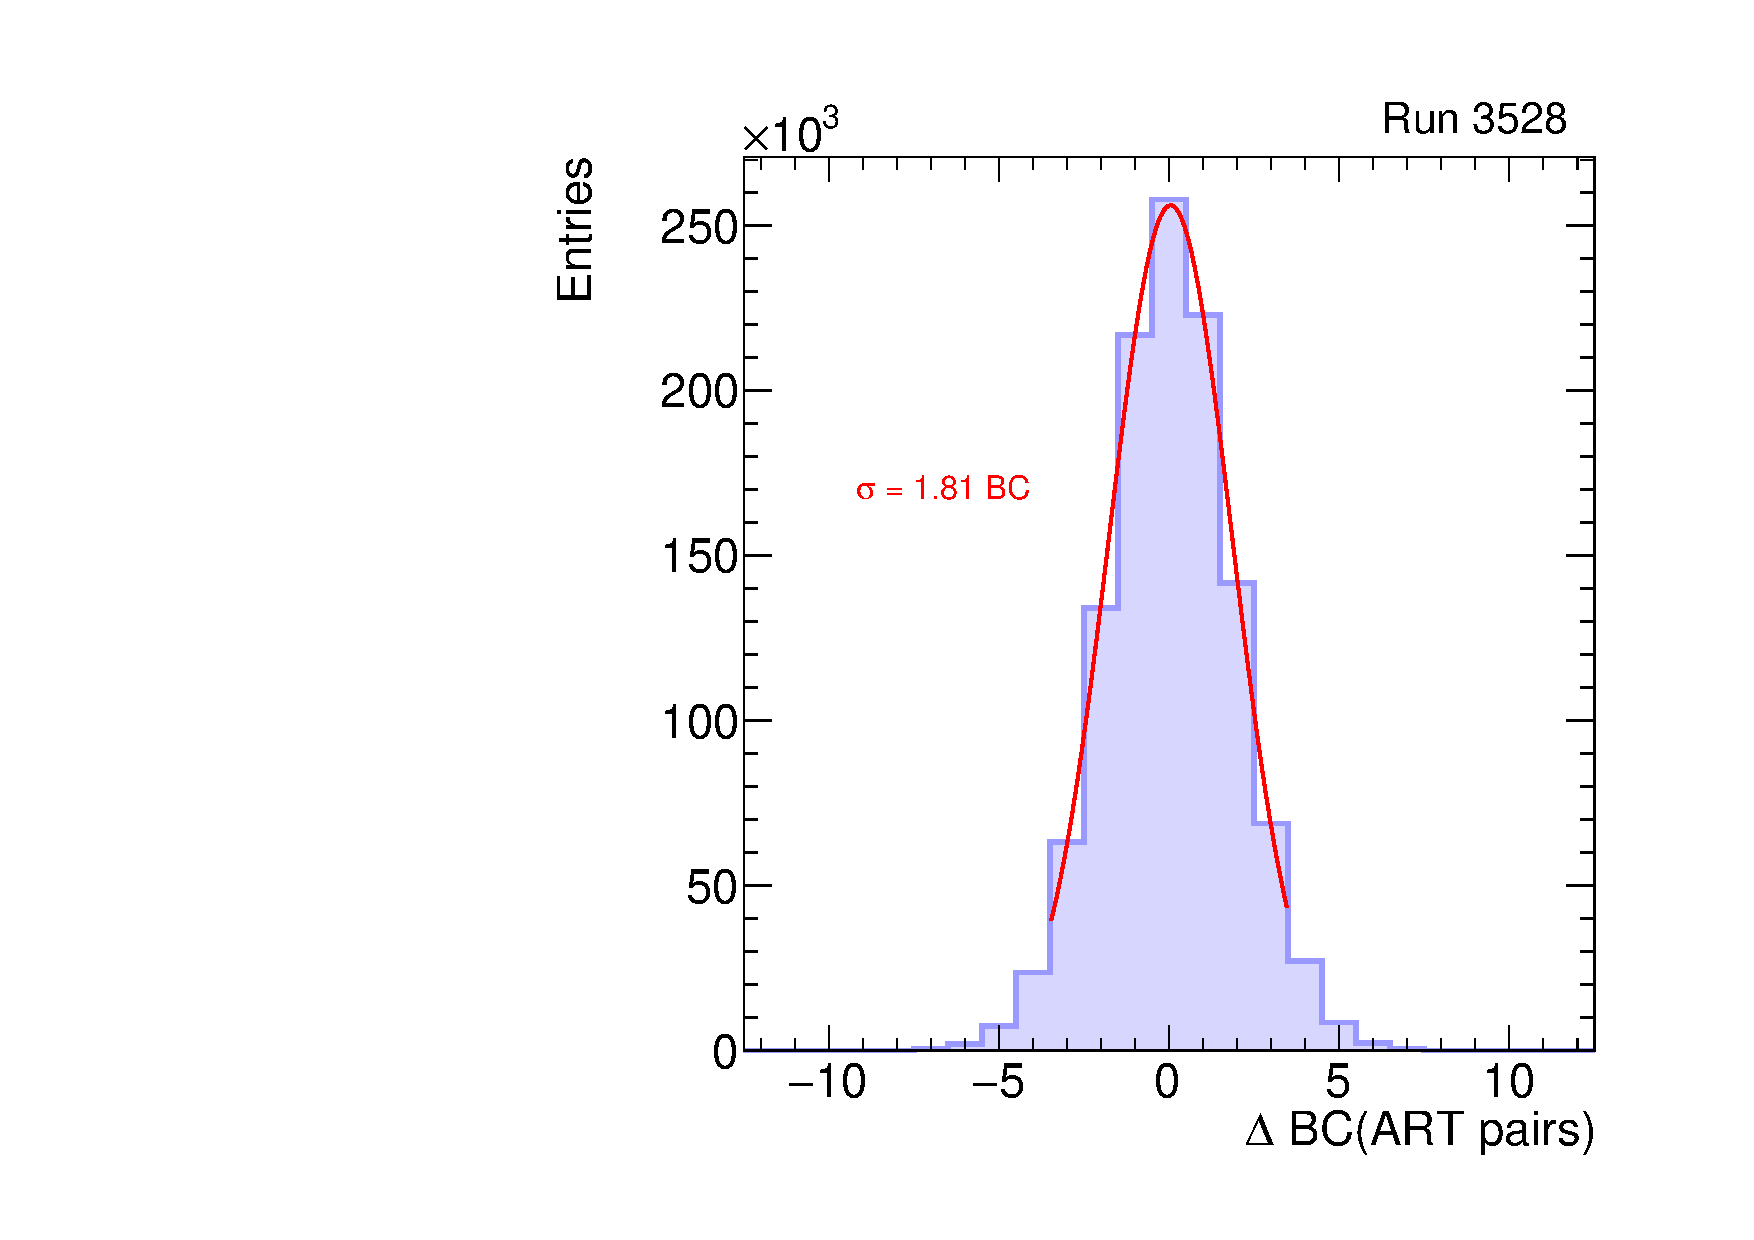
\includegraphics[width=0.3\textwidth]{figures/gbtanalysis3528/artrpairs_lin.pdf}
  \end{center}
  \vspace{-10pt}
  \caption{The $\Delta\text{BC}$ of all pairs of hits in a trigger for data collected with 200 ns (left), 100 ns (middle), and 50 ns (right) integration time in the VMM. The distribution is narrower as the integration time decreases.}
  \label{fig:integ_pairs}
\end{figure}

\begin{figure}[!htpb]
  \begin{center}
    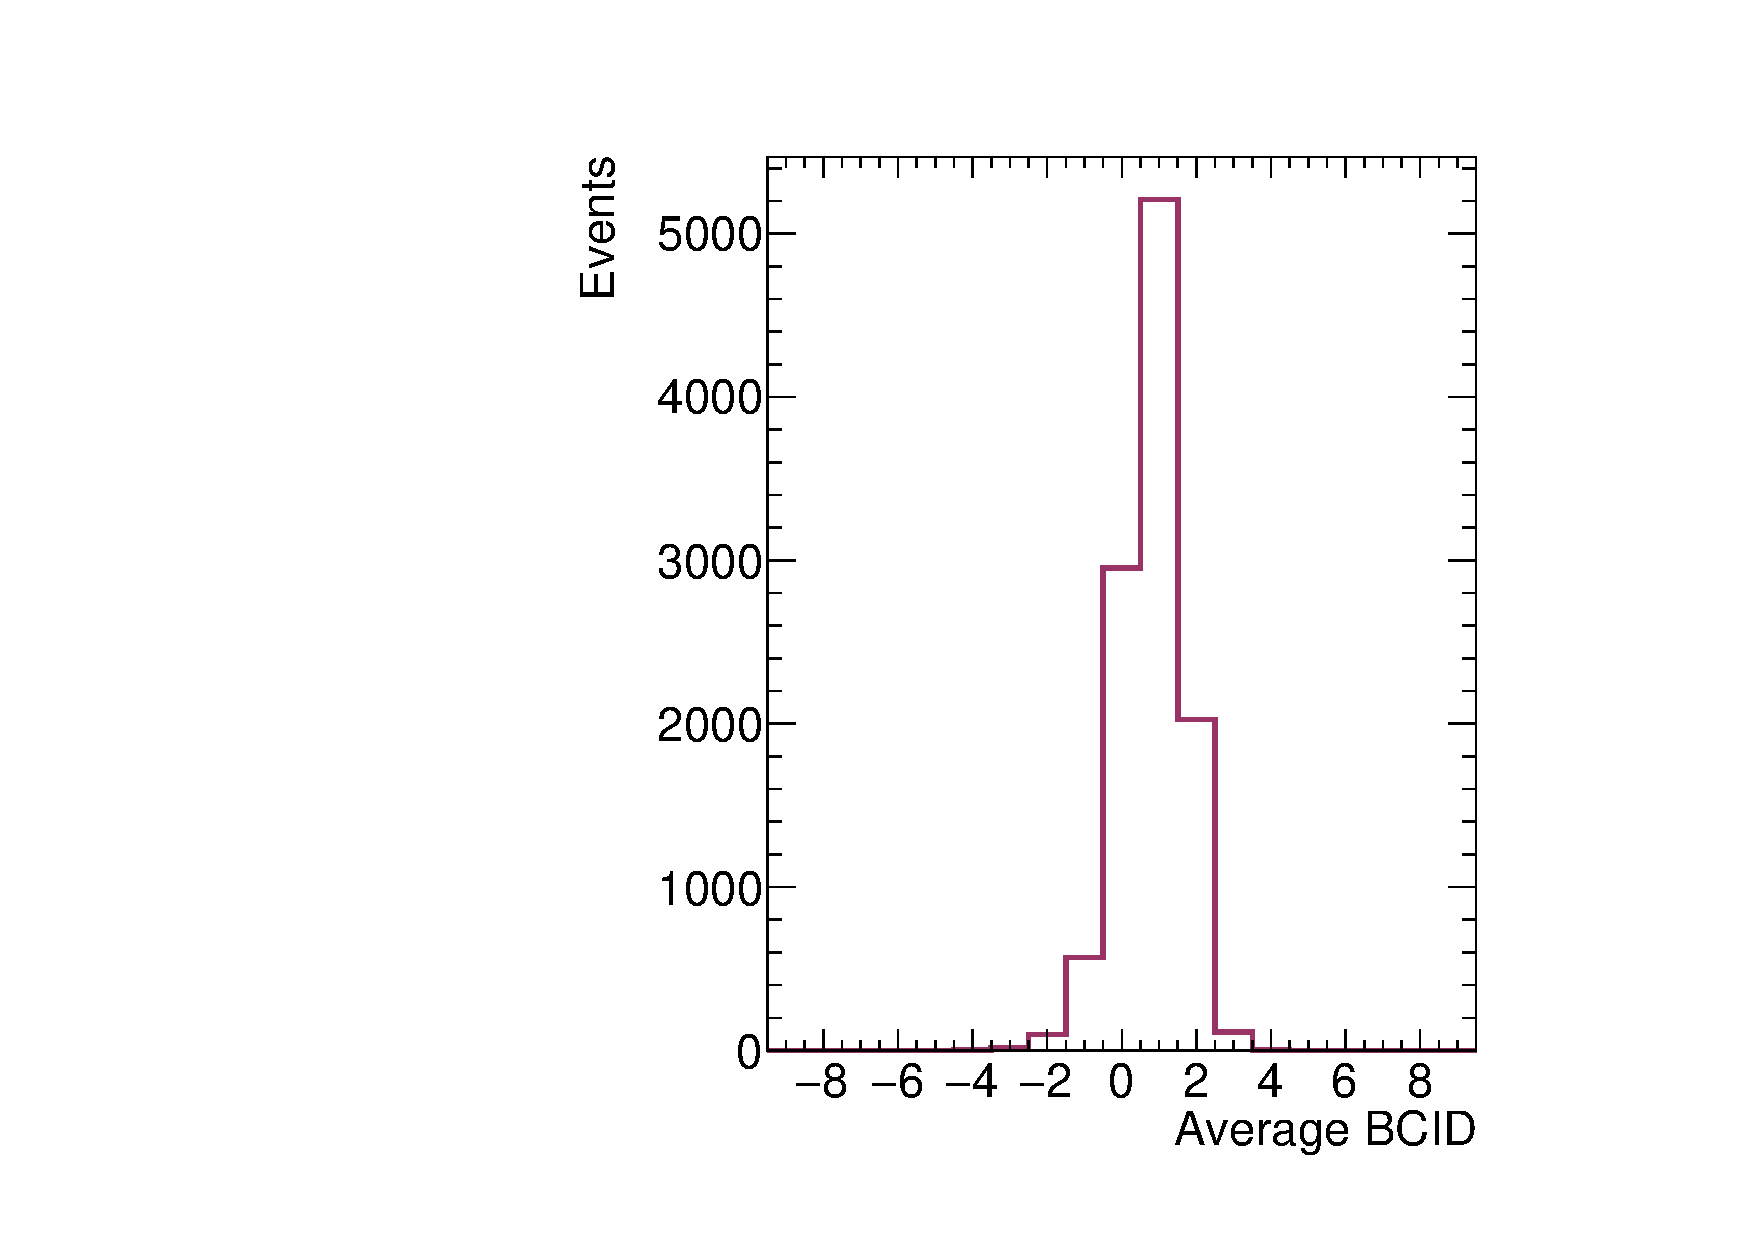
\includegraphics[width=0.3\textwidth]{figures/gbtanalysis3530/avg_BCID.pdf}
    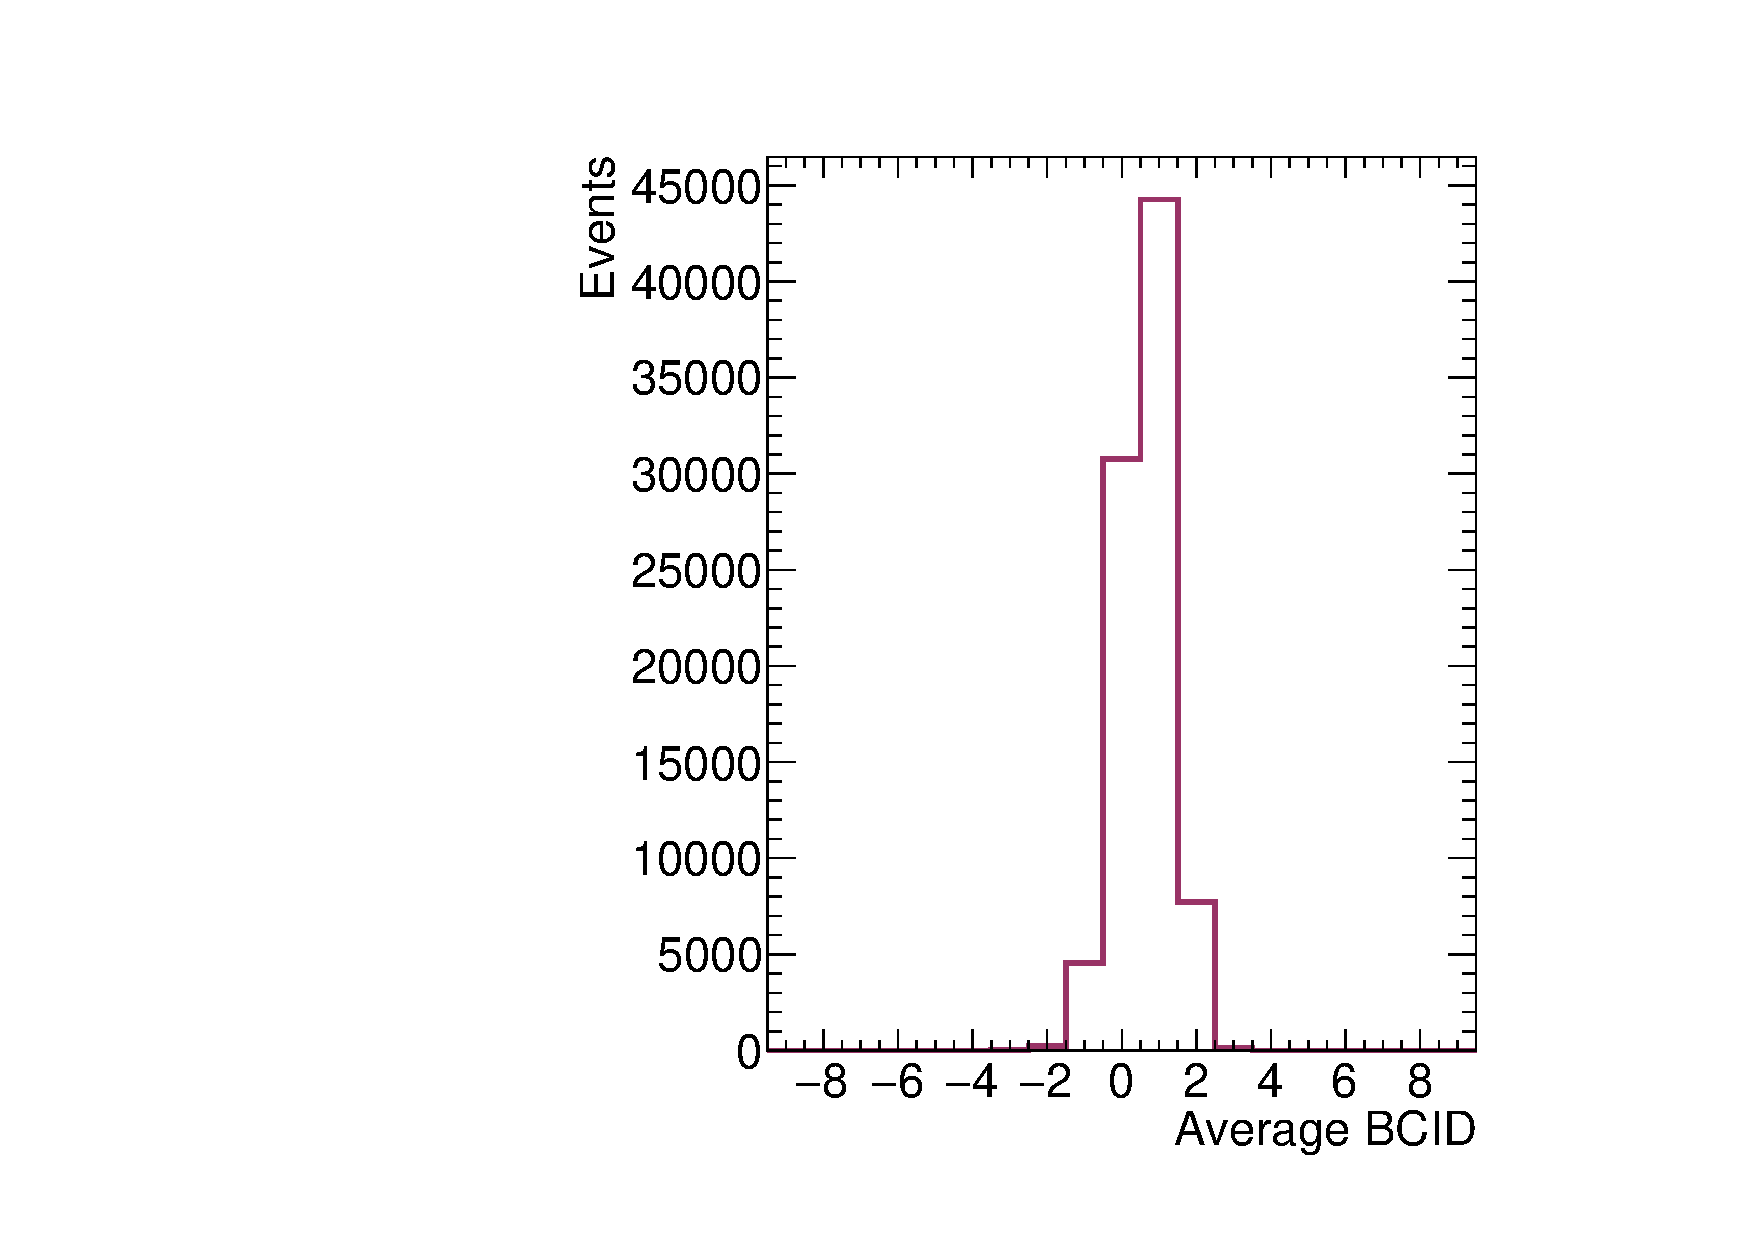
\includegraphics[width=0.3\textwidth]{figures/gbtanalysis3527/avg_BCID.pdf}
    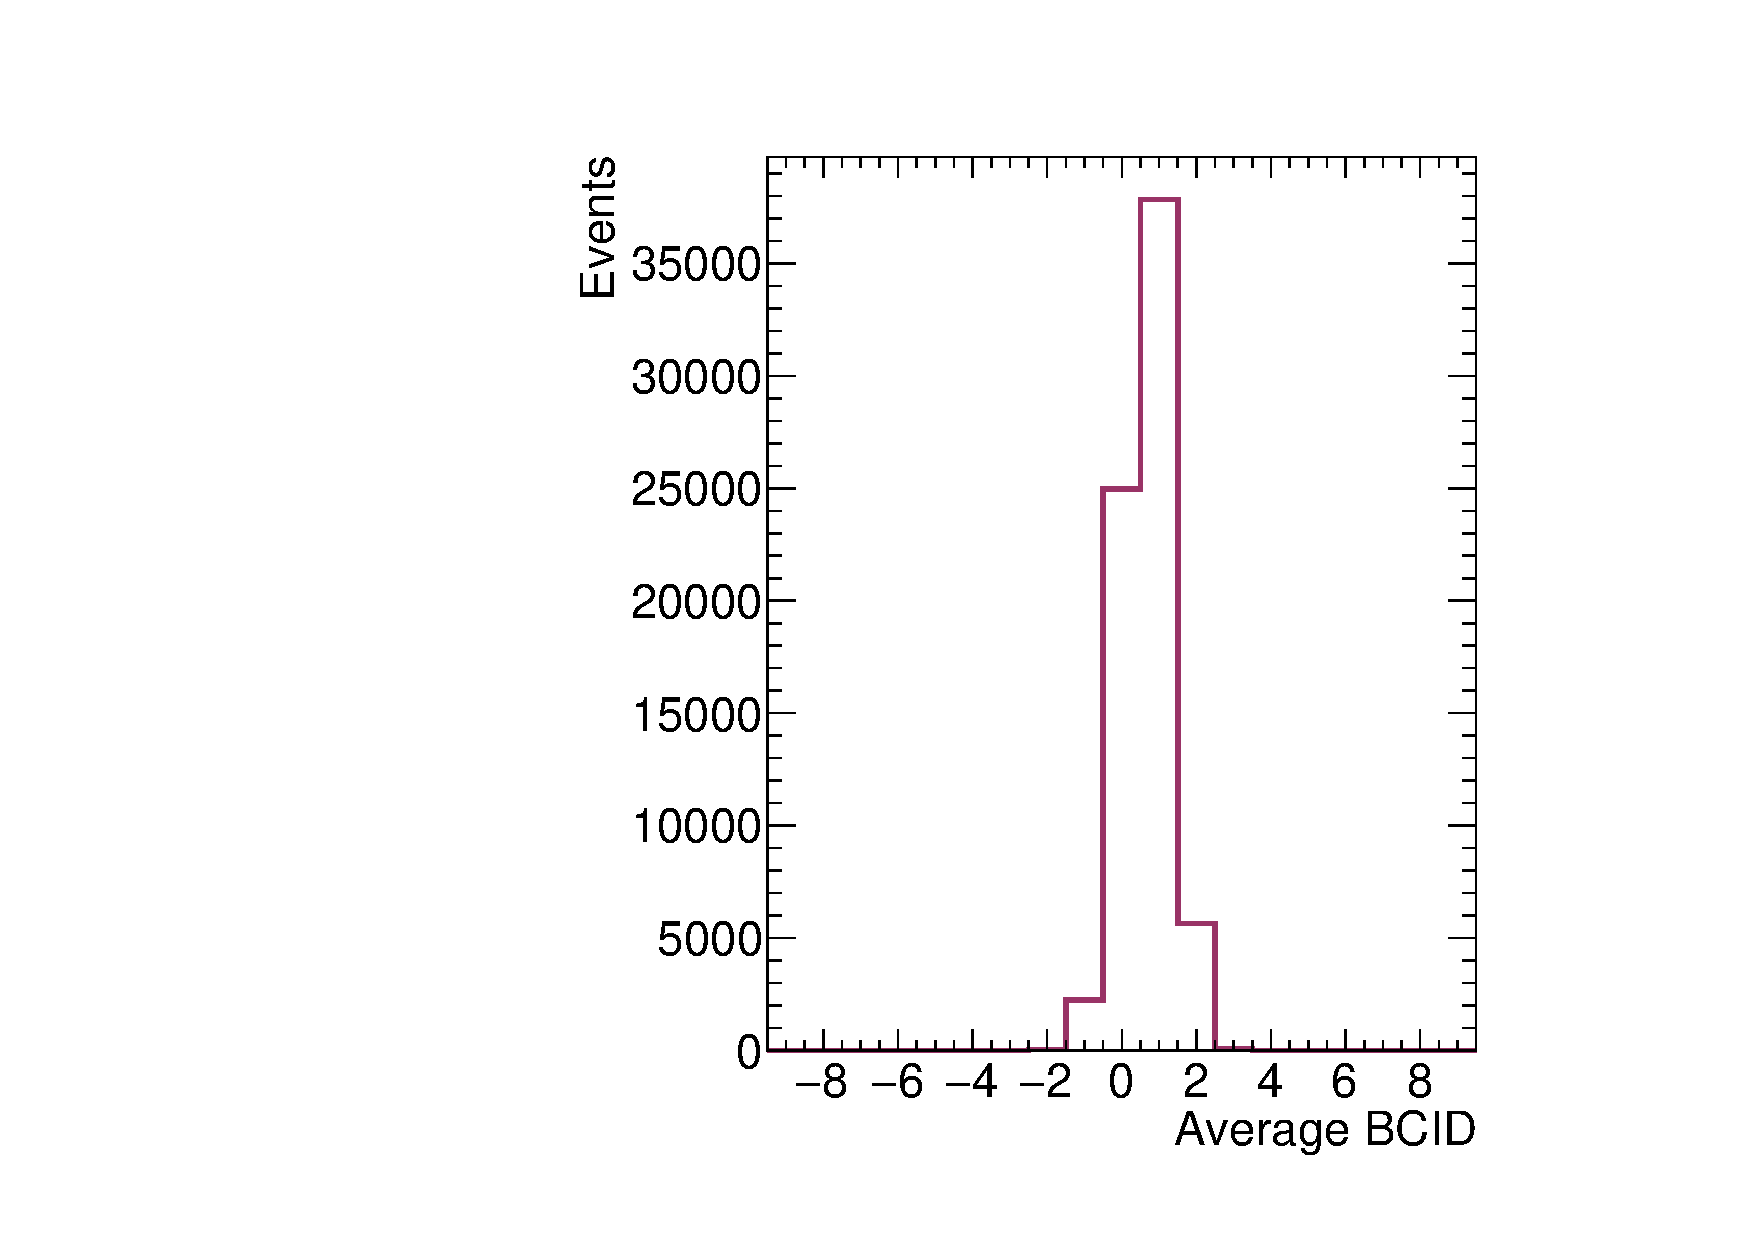
\includegraphics[width=0.3\textwidth]{figures/gbtanalysis3528/avg_BCID.pdf}
  \end{center}
  \vspace{-10pt}
  \caption{The time resolution of the MMTP relative to the scintillator, where the BC of the trigger is defined as the average BCID of the ART hits, for data collected with 200 ns (left), 100 ns (middle), and 50 ns (right) integration time in the VMM.}
  \label{fig:integ_avg_bc}
\end{figure}

\begin{figure}[!htpb]
  \begin{center}
    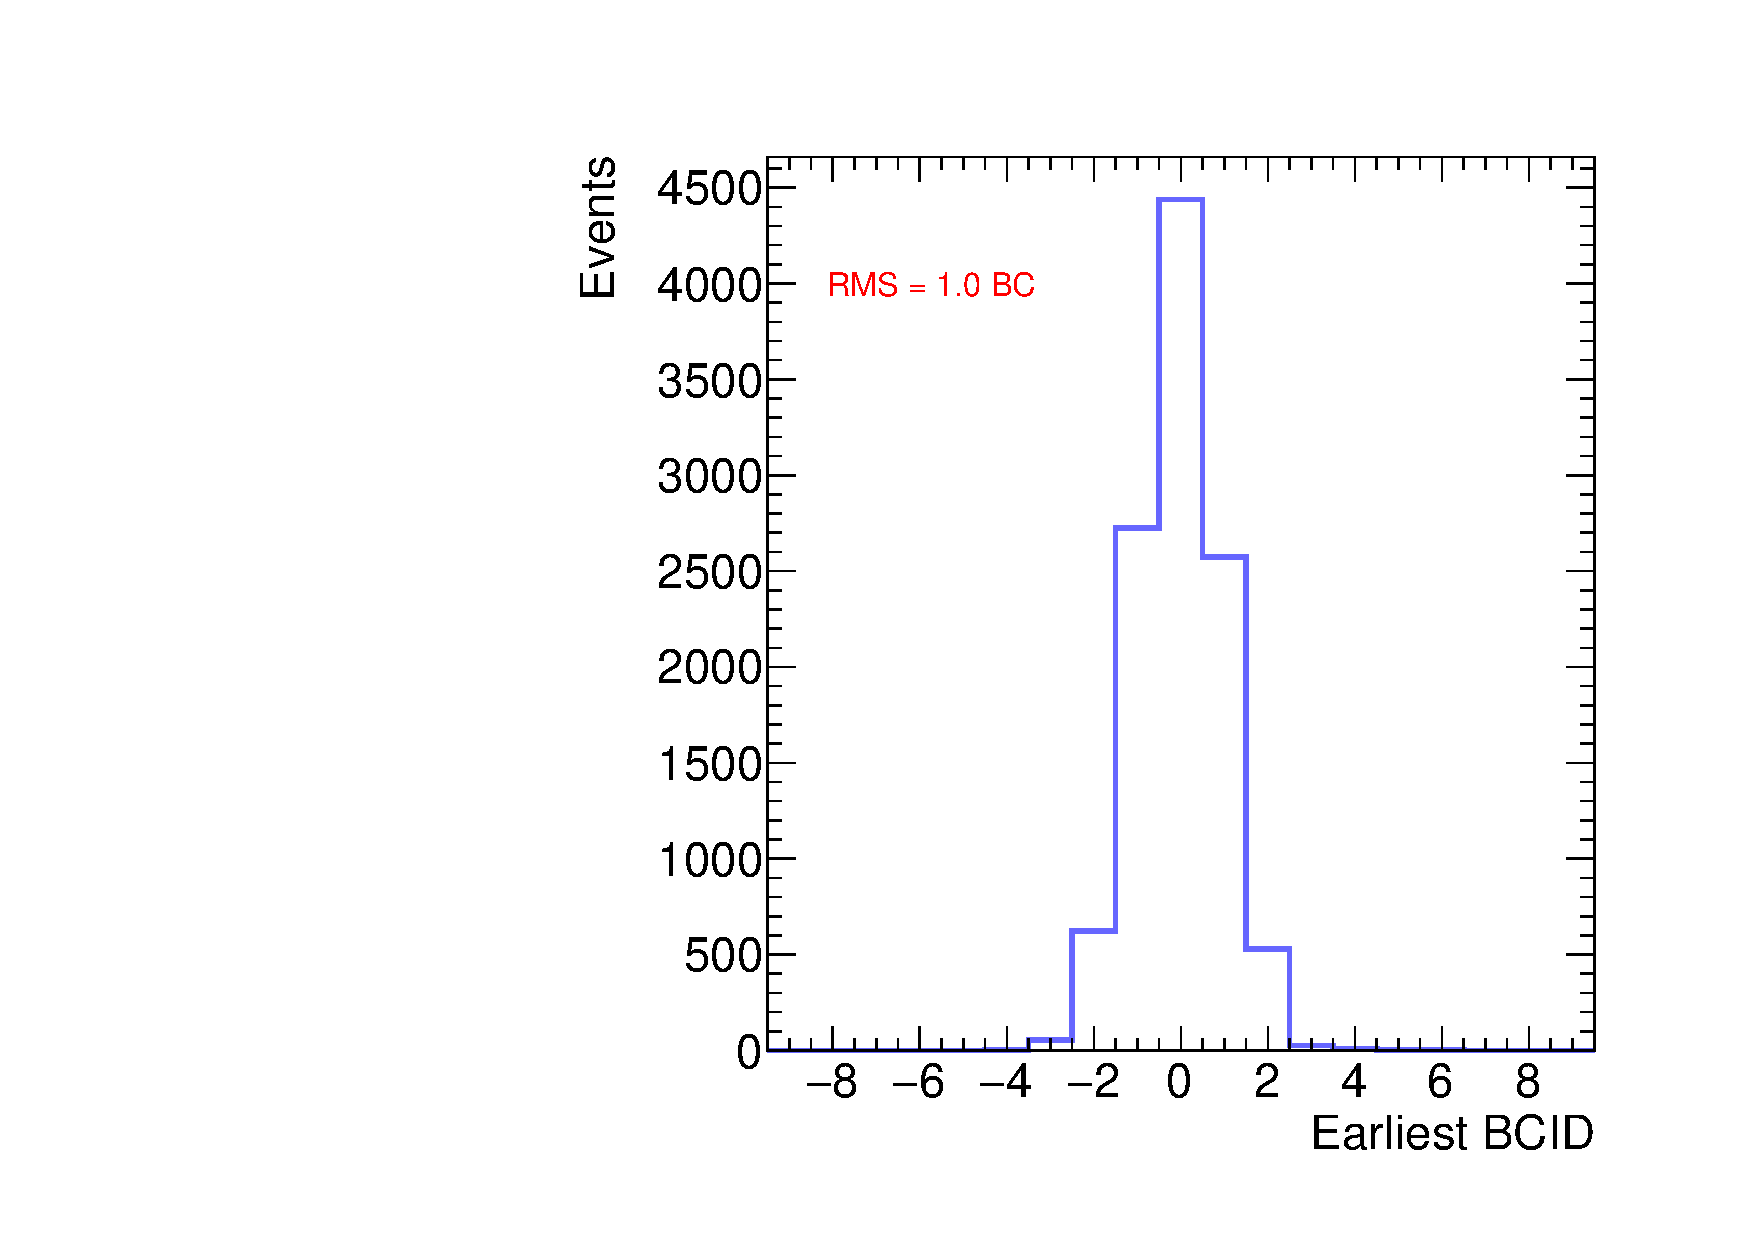
\includegraphics[width=0.3\textwidth]{figures/gbtanalysis3530/earliest_BCID.pdf}
    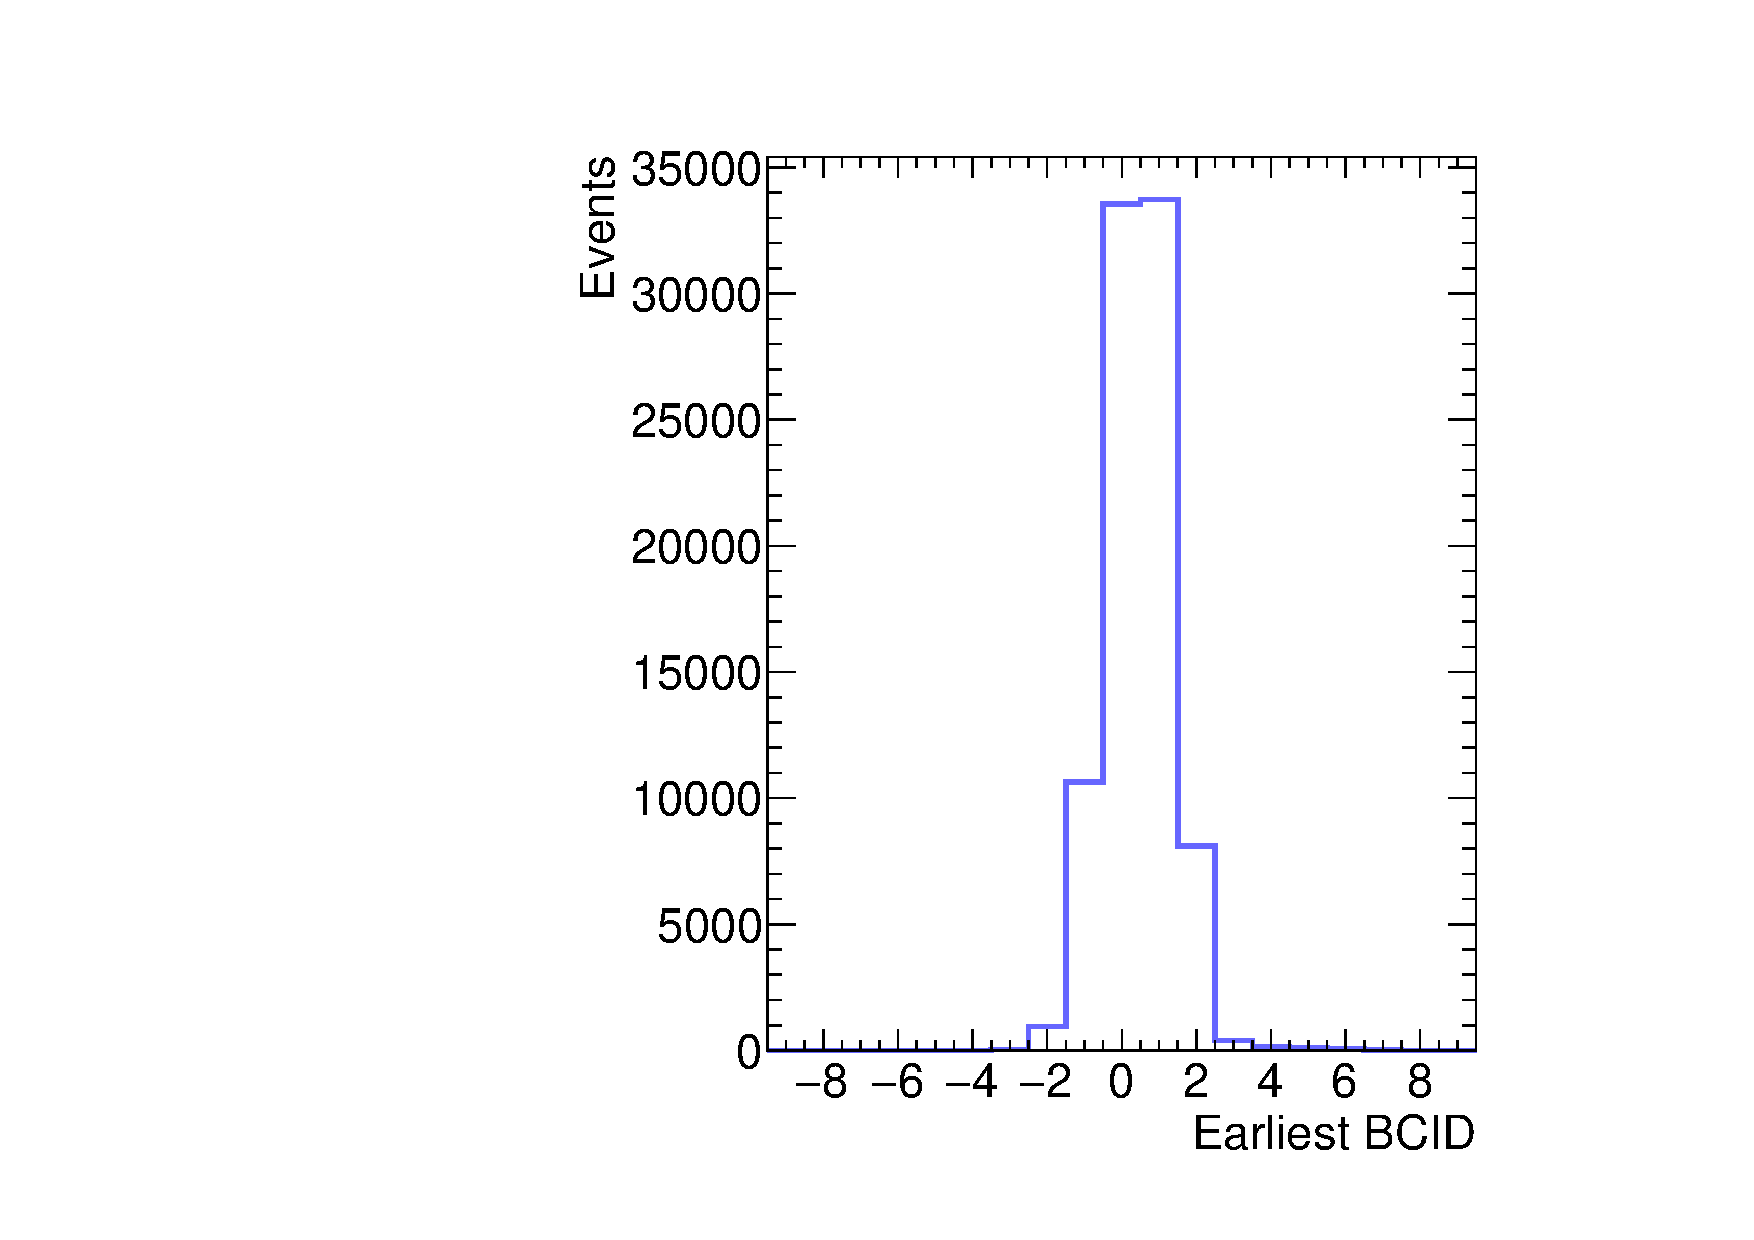
\includegraphics[width=0.3\textwidth]{figures/gbtanalysis3527/earliest_BCID.pdf}
    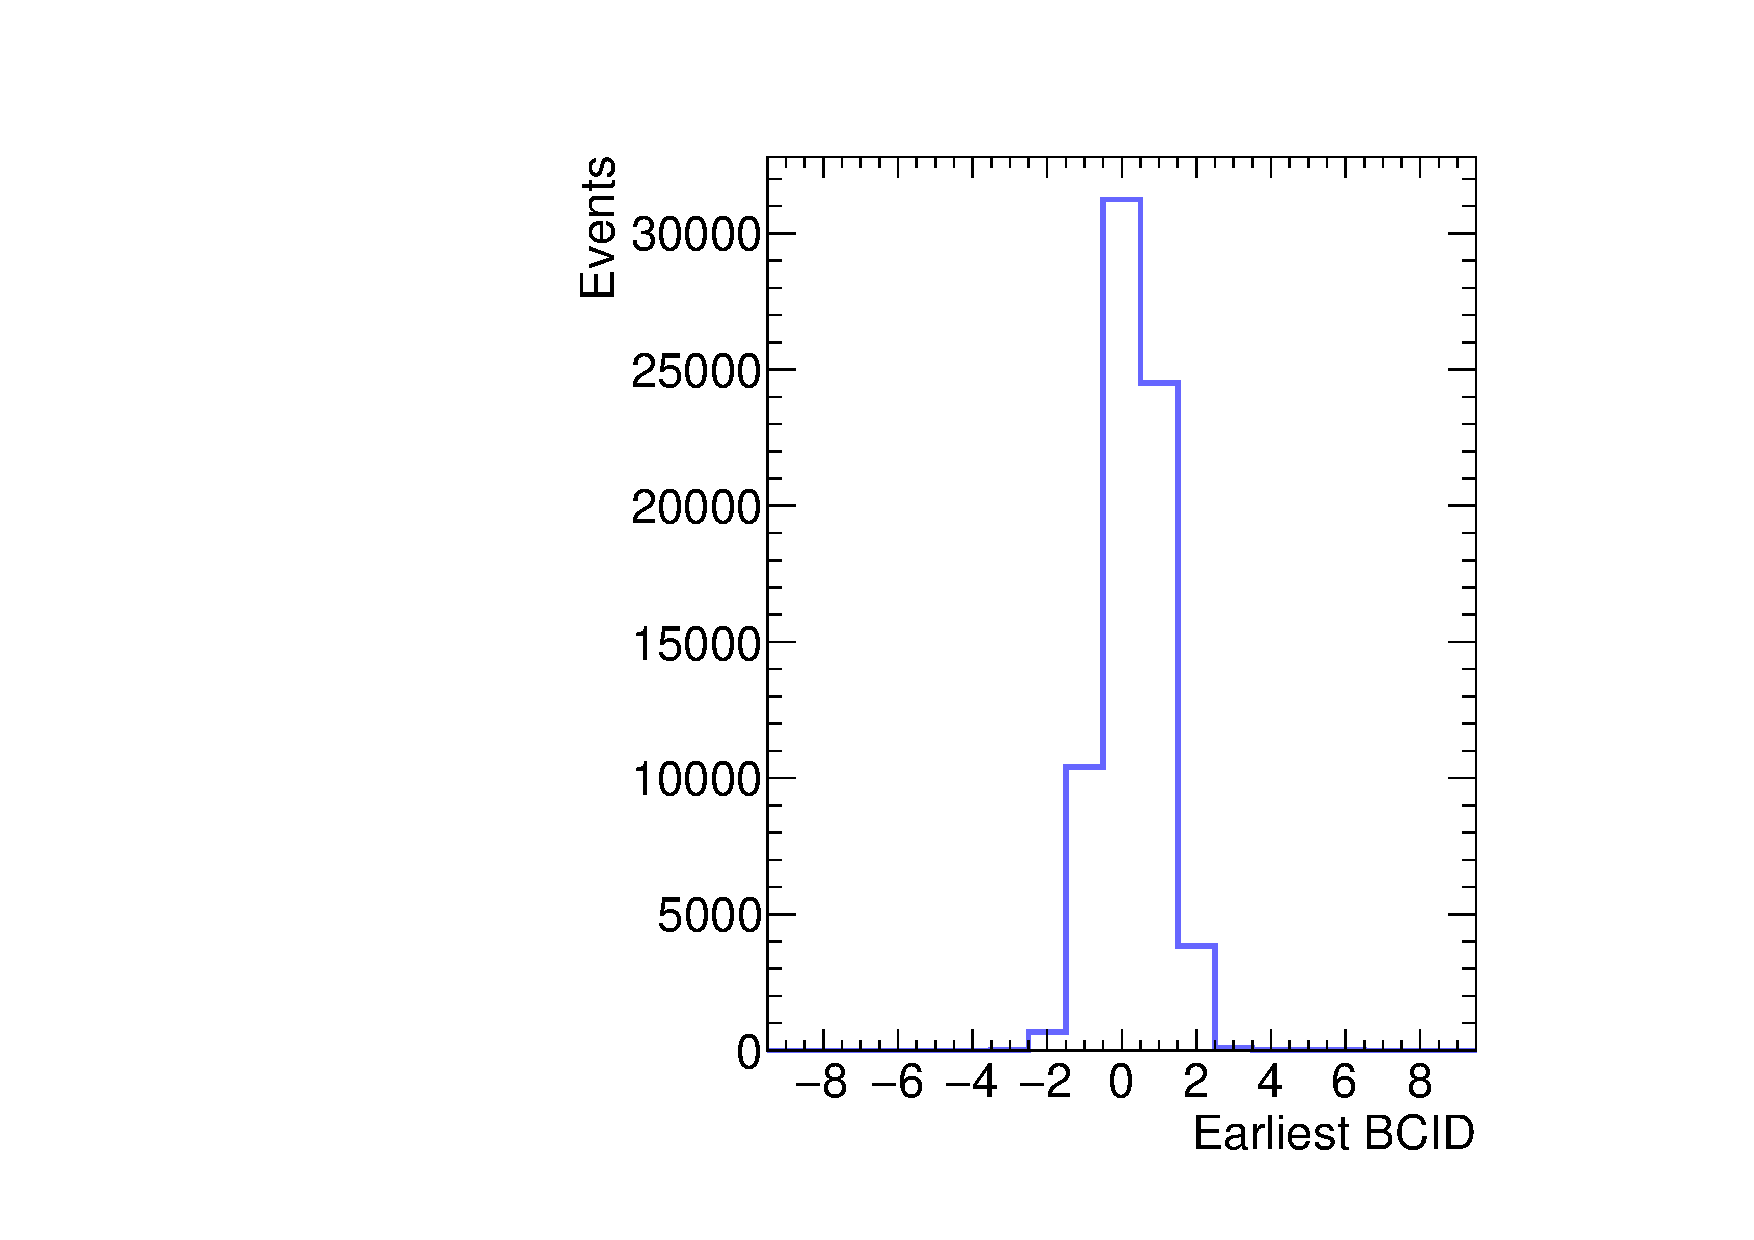
\includegraphics[width=0.3\textwidth]{figures/gbtanalysis3528/earliest_BCID.pdf}
  \end{center}
  \vspace{-10pt}
  \caption{The time resolution of the MMTP relative to the scintillator, where the BC of the trigger is defined as the earliest BCID of the ART hits, for data collected with 200 ns (left), 100 ns (middle), and 50 ns (right) integration time in the VMM.}
  \label{fig:integ_avg_earliest}
\end{figure}


